%!TEX TS-program = xelatex

%\pdfoutput=1

% IRI report class
%\documentclass{iritr}
%\IRIreport{16}{02}
%\coriri{Joan Sol\`a}{1 7337}{jsola}

% article class
\documentclass[12pt]{ctexart}
\usepackage[T1]{fontenc}
%\usepackage{a4wide}
\usepackage{geometry}
\geometry{
    a4paper,
    top=30mm,
    bottom=30mm,
    left=25.4mm,
    right=25.4mm,
    textwidth =6.375 true in % Width of text line.
}

\usepackage{amsfonts, amssymb, amsmath} 
\usepackage[english]{babel}
%\usepackage{subfigure}
%\usepackage[xetex]{graphicx}
\usepackage{multirow}
\usepackage{bm} % bold greek symbols via \bm command instead of \bf.
\usepackage{cancel}

\usepackage{caption}
\captionsetup{margin=10pt}
\captionsetup{font=small}
%\captionsetup{labelfont=bf}

%\usepackage{cite}
\usepackage{natbib}

% Customization packages
\usepackage{customCommands} % Joan Sola's macros
\usepackage{eufrak}

% A better \pm symbol
\usepackage{tikz}
\renewcommand{\pm}{\mathbin{\tikz [x=1.4ex,y=1.4ex,line width=.1ex] \draw (0.0,0) -- (1.0,0) (0.5,0.1) -- (0.5,1.0) (0.0,0.55) -- (1.0,0.55);}}%

\renewcommand\Re{\operatorname{Re}}
\renewcommand\Im{\operatorname{Im}}

% Emphasized equations
\usepackage{empheq}
\newcommand*\widefbox[1]{\fbox{\hspace{1em}#1\hspace{1em}}}

% Comments
\newcommand{\COM}[1]{{\color{red}#1}}
%\renewcommand{\COM}[1]{}

% Define a few useful shortcuts
\newcommand{\pv}{\bfp_v}
\renewcommand{\qv}{\bfq_v}
\newcommand{\qI}{\bfq_{{\,}_{\bf 1}}}
\newcommand{\q}{\,\bfq}
\newcommand{\dq}{\,\dot\bfq}
\newcommand{\ddq}{\,\ddot\bfq}
\newcommand{\dddq}{\,\dddot\bfq}
\newcommand{\ddddq}{\,\ddddot\bfq}
\newcommand{\w}{\,\bfomega}
\newcommand{\aw}{\,\ol\bfomega}
\newcommand{\dw}{\,\dot\bfomega}
\newcommand{\e}{&=}
\newcommand{\nw}{\norm{\bfomega}}
\newcommand{\Q}[1]{[#1]}
\newcommand{\QL}[1]{\Q{#1}_L}
\newcommand{\QR}[1]{\Q{#1}_R}
\newcommand{\bth}{\bftheta}
\newcommand{\dth}{\delta\bftheta}
\newcommand{\nth}{\norm{\bftheta}}
\newcommand{\te}{\triangleq}


\usepackage[	bookmarks,%
			colorlinks = true,%
			linkcolor = black,%
			citecolor = blue,%
			pdfauthor = {Joan\ Sola},%
			pdftitle = {误差状态卡尔曼滤波器的四元数动力学},%
			xetex
			]{hyperref} 
			
\setcounter{tocdepth}{3}


\title{误差状态卡尔曼滤波器的四元数动力学}
\author{Joan Sol\`a}
\date{October 12, 2017}



%%%%%%%%%%%%%%%%%%%%%%%%%%%%%%%%%%%%%%%%%%%%%%%%%%%%%%%%%%%%%%%%%

\begin{document}
\maketitle

\tableofcontents

%%%%%%%%%%%%%%%%%%%%%%%%%%%%%%%%%%%%%%%%%%%%%%%%%%%%%%%%%%%%%%%%%

% !TEX root = kinematics.tex

\begin{abstract}

本文对 3D 空间中与四元数和旋转有关的概念和公式进行了详尽的修正,并将其正确地应用于误差状态 Kalman 滤波器等估计引擎中。

本文深入研究了旋转群及其 Lie 结构,给出了四元数和旋转矩阵的表达式。
它特别关注旋转扰动、导数和积分的定义。
它提供了大量的直观和几何解释,帮助读者掌握 3D 旋转的内在机制。

整个教材被用来设计精确的公式,误差状态 Kalman 滤波器适合于实际应用,使用来自惯性测量单元(IMU)的信号集成。

\end{abstract}



% !TEX root = kinematics.tex


%%%%%%%%%%%%%%%%%%%%%%%%%%%%%%%%%%%%%%%%%%%%%%%%%%%%%%%%%%%%%%
\section{四元数定义和属性}

%=============================================================
\subsection{四元数的定义}

我找到的特别有吸引力的四元数的一个介绍是 Cayley-Dickson 给出的构造:
如果我们有两个复数 $A=a+bi$ 和 $C=c+di$,那么构造 $Q=A+Cj$ 并定义 $k\triangleq ij$ ,得到四元数 $\bbH$ 的空间中的一个数,
%
\begin{align}
Q = a + bi + cj + dk \in\bbH ~, \label{equ:ijkQuat}
\end{align}%
%
其中 $\{a,b,c,d\}\in\bbR$,和 $\{i,j,k\}$ 被定义为三个虚数。并且有
%
\begin{subequations}
\label{equ:quatAlgebra}
\begin{align}
i^2=j^2=k^2=ijk=-1~,
\end{align}%
%
从中我们可以得到
%
\begin{align}
ij = -ji = k ~, \quad jk=-kj=i~, \quad ki=-ik=j~.
\end{align}
\end{subequations}
%
从方程 \eqRef{equ:ijkQuat} 我们可以看出,我们可以嵌入复数数在实数和虚数中,因此在四元数的定义中,实数、虚数和复数数确实是四元数的意义上的子集,
%
\begin{align}
Q = a \in \bbR \subset \bbH~,
\Quad 
Q=bi \in \bbI \subset \bbH~,
\Quad 
Q=a+bi \in \bbZ \subset \bbH~.
\end{align}
%
同样,为了完备性,我们可以定义 $\bbH$ 的 3D 虚子空间中的数。
我们称它们为纯四元数(\emph{pure quaternions}),并且可以注意到 $\bbH_p=\Im(\bbH)$ 是纯四元数的空间,
%
\begin{align}
Q=bi+cj+dk \in\bbH_p \subset\bbH~.
\end{align}


值得注意的是,虽然单位长度的正则复数 $\bfz=e^{i\theta}$ 可以编码 2D 平面中的旋转 (用一个复数乘法,$\bfx'=\bfz\tdot\bfx$),“扩展复数”或单位长度四元数 $\bfq=e^{(u_xi+u_yj+u_zk)\theta/2}$ 编码 3D 空间中的旋转 (用两个四元数乘积, $\bfx'=\bfq\otimes\bfx\otimes\bfq^*$,正如我们在本文档后面解释的那样)。



\bigskip

{\bf 注意:} 并非所有四元数定义都相同。 
有些作者把乘积写成 $ib$ 而不是 $bi$,因此得到了 $k = ji = -ij$的性质,这就得到了 $ijk=1$ 的结果和左手四元数。 
此外,许多作者将实数部分放在最后位置,得到 $Q = ia + jb + kc + d$。
这些选择没有基本内涵差异,但使整个公式在细节上有所不同。 
请参阅 \secRef{sec:conventions} 了解进一步的解释和消除歧义。

\bigskip

{\bf 注意:} 还有一些附加的约定也使得公式在细节上有所不同。 
它们涉及我们给予旋转算子的“意义”或“解释”,即旋转向量或旋转参考系 --- 它们本质上构成相反的操作。 
请参阅 \secRef{sec:conventions} 得到有关进一步的解释和消除歧义。

\bigskip 

{\bf 注:} 在以上公开的不同约定中,本文集中讨论了 Hamilton 约定,其最显著的特性是定义方程 \eqRef{equ:quatAlgebra}。正确和有根据的消除歧义首先需要扩展大量的资料;因此,这个消除歧义内容被归入上述提到的 \secRef{sec:conventions}。


%=============================================================
\subsubsection{四元数的替代表示}
\label{sec:altQuat}

实数 + 虚数符号 $\{1,i,j,k\}$ 对于我们的目的并不总是方便的。 
%
%
如果使用代数方程 \eqRef{equ:quatAlgebra} ,四元数可以设为标量 + 向量的和,
%
\begin{align}
Q=q_w+q_xi+q_yj+q_zk
\qquad
\Leftrightarrow
\qquad
Q = q_w + \qv~,
\end{align}
%
其中 $q_w$ 被称为实数(\emph{real})或标量(\emph{scalar})部分,并且 $\qv=q_x i+q_y j+q_z k=(q_x,q_y,q_z)$ 作为虚数(\emph{imaginary})或向量(\emph{vector})部分。\footnote{\label{ftn:quatComponents}我们选择 $(w,x,y,z)$ 下标符号是因为我们对 3D 笛卡尔空间中四元数的几何性质感兴趣。 
其它文档通常使用另外的下标,如 $(0,1,2,3)$ 或 $(1,i,j,k)$,可能更适合数学解释。}%
它也可以定义为标量-向量(scalar-vector)有序对。 
%
\begin{align}
Q = \langle q_w,\qv\rangle ~.
\end{align}
%
我们通常把四元数 $Q$ 表示为4参数向量(4-vector) $\bfq$~,
%
\begin{align}
\bfq \triangleq 
\begin{bmatrix}
q_w\\\qv
\end{bmatrix}=
\begin{bmatrix}
q_w\\q_x\\q_y\\q_z
\end{bmatrix}~,
\end{align}%
%
这允许我们使用矩阵代数来处理四元数运算。
在某些情况下,我们可以通过滥用 ``$=$'' 标志来混合符号。典型的例子是实四元数(\emph{real quaternions})和纯四元数(\emph{pure quaternions}),
%
\begin{align}
\textrm{general: }
\bfq
=q_w+\qv=\begin{bmatrix}
q_w\\\qv
\end{bmatrix} \in \bbH
~,\quad
\textrm{real: }
q_w=\begin{bmatrix}
q_w\\{\bf0}_v
\end{bmatrix} \in \bbR
~,\quad
\textrm{pure: }
\qv=\begin{bmatrix}
0\\\qv
\end{bmatrix} \in \bbH_p
~.
\end{align}




%=============================================================
\subsection{四元数的主要性质}

\subsubsection{加法}

加法很简单,
%
\begin{align}
\bfp\pm\bfq = \begin{bmatrix}
p_w \\ \pv
\end{bmatrix} \pm \begin{bmatrix}
q_w \\ \qv
\end{bmatrix}
  = \begin{bmatrix}
p_w \pm q_w \\ \pv \pm \qv
\end{bmatrix}~.
\end{align}
%
通过构造,加法是可交换的(\textbf{commutative})和可结合的(\textbf{associative}),
%
%
\begin{align}
\bfp+\bfq&=\bfq+\bfp \\
\bfp+(\bfq+\bfr)&=(\bfp+\bfq)+\bfr
~.
\end{align}%
%
%Thus, the set of quaternions endowed with the sum operation form a commutative group, where the identity is the zero quaternion, $\bfq_0 = 0$, and the inverse is the negative  $-\bfq$.

\subsubsection{乘法}

乘法用 $\otimes$ 符号表示,四元数乘积需要使用原始形式方程 \eqRef{equ:ijkQuat} 和四元数代数方程 \eqRef{equ:quatAlgebra}。
将结果以向量形式写入
%
\begin{align}
\bfp\otimes\bfq = \begin{bmatrix}
p_wq_w - p_{x}q_{x} - p_{y}q_{y} - p_{z}q_{z} \\
p_wq_{x} + p_{x}q_w + p_{y}q_{z} - p_{z}q_{y} \\
p_wq_{y} - p_{x}q_{z} + p_{y}q_w + p_{z}q_{x} \\
p_wq_{z} + p_{x}q_{y} - p_{y}q_{x} + p_{z}q_w  
\end{bmatrix}~. \label{equ:quatProd}
\end{align}
%
这也可以用标量和向量部分来表示,
%
\begin{align}
\bfp\otimes\bfq = \begin{bmatrix}
p_wq_w - \pv\tr\qv \\
p_w\qv+q_w\pv+\pv\!\times\!\qv
\end{bmatrix}~, \label{equ:quatProdVec}
\end{align}
%
其中
交叉积的存在
表明四元数乘积在一般情况下是不可交换的(\textbf{not commutative}),
%
\begin{align}
\bfp\otimes\bfq\neq\bfq\otimes\bfp~.
\end{align}
%
这种一般非交换性的例外仅限于 $\pv\!\times\!\qv=0$ 当其中一个四元数是实数(实四元数)的情况, $\bfp=p_w$ 或 $\bfq=q_w$;或者当两个向量部分是平行的情况, $\pv \| \qv$。只有在这些情况下,四元数乘积才是可交换的。

四元数乘积是可结合的(\textbf{associative}),
%
\begin{align}
(\bfp\otimes\bfq)\ot\bfr = \bfp\otimes(\bfq\ot\bfr)~,
\end{align}
%
并且符合分配律(\textbf{distributive over the sum}),
%
\begin{align}
\bfp\ot(\bfq+\bfr) = \bfp\ot\bfq + \bfp\ot\bfr
\qquad \textrm{and} \qquad
%\qquad,\qquad
(\bfp+\bfq)\ot\bfr = \bfp\ot\bfr + \bfq\ot\bfr~.
\end{align}
%



两个四元数的乘积是双线性的,可以表示为两个等价的矩阵乘积,即
%
\begin{align}
\bfq_1\ot\bfq_2 = \QL{\bfq_1}\,\bfq_2 
\qquad \textrm{and} \qquad
\bfq_1\ot\bfq_2 = \QR{\bfq_2}\,\bfq_1 ~, \label{equ:quatMatProd}
\end{align}%
%
其中 $\QL{\bfq}$ 和 $\QR{\bfq}$ 分别是四元数左乘(left-product)矩阵和四元数右乘(right-product)矩阵,由方程 \eqRef{equ:quatProd} 和 \eqRef{equ:quatMatProd} 通过简单检验导出,
%
\begin{align}
\QL{\bfq} = \begin{bmatrix}
q_w &-q_x &-q_y &-q_z\\
q_x & q_w &-q_z & q_y\\
q_y & q_z & q_w &-q_x\\
q_z &-q_y & q_x & q_w\\
\end{bmatrix}, \qquad
\QR{\bfq} = \begin{bmatrix}
q_w &-q_x &-q_y &-q_z\\
q_x & q_w & q_z &-q_y\\
q_y &-q_z & q_w & q_x\\
q_z & q_y &-q_x & q_w\\
\end{bmatrix} ,
\label{equ:quatMatrixComponents}
\end{align}%
%
或者更简洁地说,从方程 \eqRef{equ:quatProdVec} 和 \eqRef{equ:quatMatProd} 开始导出,
%
\begin{align}
\QL{\bfq} = q_w\,\bfI + \begin{bmatrix}
0 & -\qv\tr \\
\qv & \hatx{\qv}
\end{bmatrix}, \qquad
\QR{\bfq} = q_w\,\bfI + \begin{bmatrix}
0 & -\qv\tr \\
\qv & -\hatx{\qv}
\end{bmatrix}~.
\label{equ:quatMatrix}
 ~
\end{align}%
%
这里,斜交算子(\emph{skew operator})\footnote{斜交算子可以在文献中以许多不同的名称和符号找到,或者与交叉算子 $\times$ 相关,或者与帽子“hat”算子 $^\wedge$ 相关,因此下面的所有形式都是等效的,
$$
\hatx{\bfa} \equiv [\bfa_\times] \equiv \bfa\!\times \equiv \bfa_\times \equiv [\bfa] \equiv \widehat{\bfa} \equiv \bfa^\wedge~.
$$
} 
%
$\hatx{\bullet}$ 产生交叉乘积矩阵,
%
\begin{align}
\hatx{\bfa} \triangleq \begin{bmatrix}
0 & -a_z & a_y \\
a_z & 0 & -a_x \\
-a_y & a_x & 0
\end{bmatrix}
\label{equ:skew}
~,
\end{align}
%
这是一个斜对称矩阵, $\hatx{\bfa}\tr=-\hatx{\bfa}$,相当于叉积,即, 
%
\begin{align}
\hatx{\bfa}\bfb = \bfa\tcross\bfb~,\quad \forall\, \bfa,\bfb\in\bbR^3 ~.  
\end{align}



最后,因为
%
\begin{align}
(\bfq\ot\bfx)\ot\bfp = \QR{\bfp}\,\QL{\bfq}\,\bfx 
\qquad \textrm{and} \qquad
\bfq\ot(\bfx\ot\bfp) = \QL{\bfq}\,\QR{\bfp}\,\bfx
~,
\end{align}
%
我们有关系
%
\begin{align}
\QR{\bfp}\,\QL{\bfq} = \QL{\bfq}\,\QR{\bfp}~,
\label{equ:PQ_commute}
\end{align}
%
这就是左乘和右乘四元数矩阵是可交换的。
这些矩阵的进一步性质在 \secRef{sec:isoclinic} 提供。


赋予乘积运算 $\otimes$ 的四元数构成一个非交换群。 
群的元素特征值 $\bfq_1=1$ 和逆式 $\bfq\inv$ 在下面进行探讨。

\subsubsection{特征值}

特征四元数 $\qI$ 相对于乘积是这样 $\qI\otimes\bfq=\bfq\otimes\qI=\bfq$。
它对应于表示为四元数的实数乘积特征值 `1' 。
%
\begin{align*}
\qI = 1 = \begin{bmatrix}
1 \\ {\bf0}_v
\end{bmatrix} ~.
\end{align*}


\subsubsection{共轭}

四元数的共轭定义为
%
\begin{align}
\bfq^*\triangleq q_w-\qv=\begin{bmatrix}
q_w \\ -\qv
\end{bmatrix}
~.
\end{align}
%
有属性为
%
\begin{align}
\bfq\otimes\bfq^* = \bfq^*\otimes\bfq 
=q_w^2 +q_x^2 +q_y^2 +q_z^2
= \begin{bmatrix}
q_w^2 +q_x^2 +q_y^2 +q_z^2 \\ {\bf0}_v
\end{bmatrix}
~,
\end{align}
%
和
%
\begin{align}
(\bfp\ot\bfq)^* = \bfq^*\ot\bfp^* 
~.
\end{align}%


\subsubsection{范数}

四元数的范数定义为
%
\begin{align}\label{equ:q_norm}
\norm{\bfq} \triangleq \sqrt{\bfq\otimes\bfq^*} = \sqrt{\bfq^*\otimes\bfq} = \sqrt{q_w^2 +q_x^2 +q_y^2 +q_z^2 } ~\in \bbR ~.
\end{align}
%
它有属性
%
\begin{align}
\norm{\bfp\ot\bfq} = \norm{\bfq\ot\bfp} = \norm{\bfp}\norm{\bfq}~. \label{equ:norm_prod}
\end{align}•

\subsubsection{逆}

逆四元数 $\bfq\inv$ 使得四元数乘以其逆得到特征值,
%
\begin{align}
\bfq\otimes\bfq\inv = \bfq\inv\otimes\bfq = \qI~.
\end{align}
%
它可以用下式计算
%
\begin{align}
\bfq\inv = \bfq^*/\norm{\bfq}^2~.
\end{align}

\subsubsection{单位或规范化四元数}

对于单位四元数, $\norm{\bfq}=1$,因此
%
\begin{align}
\bfq\inv = \bfq^*~.
\end{align}


当将单位四元数解释为方向规范或旋转算子时,此属性意味着可以使用共轭四元数完成逆旋转。单位四元数总是可以用这种形式写为,
%
\begin{align}
\bfq = \begin{bmatrix}
\cos\theta \\ \bfu\sin\theta
\end{bmatrix}
~,
\end{align}
%
其中 $\bfu = u_x i + u_y j + u_z k$ 是单位向量,并且 $\theta$ 是标量。 

从方程 \eqRef{equ:norm_prod} 开始,赋予乘积操作 $\otimes$ 形式的单位四元数形成一个非交换群,其中逆与共轭重合。 


\subsection{附加四元数属性}

\subsubsection{四元数交换器}

四元数交换器(\emph{commutator})定义为 $[\bfp,\bfq]\triangleq\bfp\ot\bfq-\bfq\ot\bfp$。我们从方程 \eqRef{equ:quatProdVec} 得到,
%
\begin{align}
\bfp\ot\bfq-\bfq\ot\bfp = 2\,\pv\tcross\qv
~.
\label{equ:quatCommutator}
\end{align}
%
这有一个平凡的结果,
%
\begin{align}
\pv\ot\qv-\qv\ot\pv = 2\,\pv\tcross\qv
~.
\label{equ:quatCommutatorPure}
\end{align}
%
稍后我们将使用此属性。


\subsubsection{纯四元数的乘积}

纯四元数是那些实部或标量部为零的四元数, $Q=\qv$ 或 $\bfq=[0,\qv]$。 我们从方程 \eqRef{equ:quatProdVec} 得到,
%
\begin{align}
\pv\ot\qv 
= -\pv\tr\qv + \pv\tcross\qv
= \begin{bmatrix}
-\pv\tr\qv \\
\pv\tcross\qv
\end{bmatrix}~.
\label{equ:quatProdPure}
\end{align}
%
这意味着
%
\begin{align}
\qv\ot\qv = -\qv\tr\qv = -\norm{\qv}^2~,
\label{equ:quatPureSquared}
\end{align}
%
并且对于纯酉四元数 $\bfu\in\bbH_p,~ \norm{\bfu}=1$,
%
\begin{align}
\bfu\ot\bfu = -1
~,
\end{align}
%
这类似于标准的假想情况, $i\cdot i=-1$.

\subsubsection{纯四元数的自然数幂}

让我们用四元数乘积 $\ot$定义 $\bfq^n, ~n\in\bbN$ 为 $\bfq$ 的 $n$次幂。
然后,如果 $\bfv$ 是纯四元数,我们让 $\bfv=\bfu\,\theta$,用 $\theta=\norm{\bfv}\in\bbR$ 和 $\bfu$ 的,我们从方程 \eqRef{equ:quatPureSquared} 得到循环模式
%
\begin{align}
\bfv^2 = -\theta^2 \quad,\quad
\bfv^3 = -\bfu\,\theta^3 \quad,\quad
\bfv^4 = \theta^4 \quad,\quad
\bfv^5 = \bfu\,\theta^5 \quad,\quad
\bfv^6 = -\theta^6 \quad,\quad
\cdots
\label{equ:qvPowers}
\end{align}
%
%并且对于纯酉四元数 $\bfu$,这将减少到模式
%%
%\begin{align}
%\bfu^2 = -1 	\quad,\quad
%\bfu^3 = -\bfu 	\quad,\quad
%\bfu^4 = 1 		\quad,\quad
%\bfu^5 = \bfu 	\quad,\quad
%\bfu^6 = -1 	\quad,\quad
%\cdots
%\label{equ:uPowers}
%\end{align}




\subsubsection{纯四元数的指数}

%我们用实数指数的一个推广定义了一般四元数的指数,目的是捕捉其大部分性质。
四元数指数是四元数上类似于普通指数函数的函数。 
与实数指数情形一样,它被定义为绝对收敛幂级数,
%
\begin{align}
e^\bfq
\triangleq \sum_{k=0}^\infty \frac{1}{k!}\bfq^k \quad \in \bbH
~.
\label{equ:quatExpSeries}
\end{align}
%
显然,实四元数的指数与普通指数函数完全一致。 

更有趣的是,纯四元数 $\bfv=v_xi+v_yj+v_zk$~ 的指数是一个新的四元数,定义为
%
\begin{align}
e^\bfv
= \sum_{k=0}^\infty \frac{1}{k!}\bfv^k \quad \in \bbH
~.
\label{equ:pureQuatExpSeries}
\end{align}
%
设 $\bfv=\bfu\,\theta$,用 $\theta=\norm{\bfv}\in\bbR$ 和 $\bfu$ 的酉,考虑方程 \eqRef{equ:qvPowers} ,我们将级数中的标量项和向量项分组, 
%
\begin{align}
e^{\bfu\theta} 
&= \left(1-\frac{\theta^2}{2!}+\frac{\theta^4}{4!}+\cdots\right) + \left(\bfu\theta - \frac{\bfu\theta^3}{3!}+\frac{\bfu\theta^5}{5!}+\cdots\right)
\end{align}
%
从中分别识别出 $\cos\theta$ 和 $\sin\theta$的级数。
% 
%
\footnote{我们提示 $\cos \theta = 1 - \theta^2/2! + \theta^4/4! - \cdots$,和 $\sin \theta =  \theta - \theta^3/3! + \theta^5/5! - \cdots$。}
%
其结果为
%
\begin{align}
e^\bfv
= e^{\bfu\,\theta} 
= \cos\theta + \bfu\sin\theta = \begin{bmatrix}
\cos\theta \\ \bfu\sin\theta 
\end{bmatrix} ~,
\label{equ:EulerFormulaQuat}
\end{align}
%
这是 Euler 公式的一个漂亮的扩展, $e^{i\theta}=\cos\theta+i\sin\theta$,定义为虚数。 
%
注意,由于 $\norm{e^{\bfv}}^2=\cos^2\theta+\sin^2\theta=1$,纯四元数的指数是一个单位四元数。
还要注意性质,
%
\begin{align}
e^{-\bfv} = \left(e^{\bfv}\right)^*
~.
\end{align}

对于小角度四元数,在方程 $\bfu=\bfv/\norm{\bfv}$ 中,我们通过 $\sin\theta$ 和 $\cos\theta$ 的泰勒级数表达和截断的级数,得到了不同程度的近似,避免了除以零的问题。
%
\begin{align}
e^\bfv 
\approx
\begin{bmatrix}
1-\theta^2/2 \\ \bfv\big(1-\theta^2/6\big) 
\end{bmatrix}
\approx
\begin{bmatrix}
1 \\ \bfv 
\end{bmatrix}
\xrightarrow[\theta\to 0]{}
\begin{bmatrix}
1 \\ {\bf0}
\end{bmatrix}
~.
\end{align}
%


\subsubsection{一般四元数的指数}


由于四元数乘积的非交换性,我们不能为一般的四元数 $\bfp$ 和 $\bfq$ 写出 $e^{\bfp+\bfq}=e^\bfp e^\bfq $。然而,当任一乘积成员是标量时,交换性成立,因此,
%
\begin{align}
e^\bfq = e^{q_w+\qv} = e^{q_w}\,e^{\qv} ~.
\end{align}
%
然后,对 $\bfu\theta=\qv$ 使用方程 \eqRef{equ:EulerFormulaQuat} ,我们得到
%
\begin{align}\label{equ:expGeneralQuat}
e^\bfq 
= e^{q_w}\begin{bmatrix}
\cos\norm{\qv} \\ \frac{\qv}{\norm{\qv}}\sin\norm{\qv} 
\end{bmatrix}~.
\end{align}
%


\subsubsection{单位四元数的对数}
\label{sec:qlog}

很快就能看出,如果 $\norm{\bfq}=1$,
%
\begin{align}\label{equ:qlog}
\log \bfq = \log (\cos \theta + \bfu \sin\theta) = \log(e^{\bfu\,\theta}) = \bfu\,\theta = \begin{bmatrix}
0 \\ \bfu\,\theta
\end{bmatrix}
~,
\end{align}
%
也就是说,单位四元数的对数是纯四元数。通过反转方程 \eqRef{equ:EulerFormulaQuat} 容易获得角-轴(angle-axis)数值,
%
\begin{align}
\bfu &= \qv / \norm{\qv} \\
\theta &= \arctan(\norm{\qv},q_w)
~.
\end{align}
%
对于小角度四元数,我们通过 $\arctan(x)$ 的泰勒级数表达和截断,\footnote{我们提示 $\arctan x = x - x^3/3 + x^5/5 - \cdots$,和 $\arctan(y,x)\equiv\arctan(y/x)$。} 获得不同程度的近似,避免了除以零的问题。
%
\begin{align}
\log(\bfq) 
= \bfu\theta 
&= \qv\frac{\arctan({\norm{\qv},q_w})}{\norm{\qv}} 
\approx \frac{\qv}{q_w} \left(1 - \frac{\norm{\qv}^2}{3q_w^2}\right)
\approx \bfq_v
\xrightarrow[\theta\to 0]{}
{\bf 0}
~.
\end{align}
%
%其中,对于 $\theta\to 0$ 的极限,趋向于 $\log(\bfq)=\bfq_v$.



\subsubsection{一般四元数的对数}

通过扩展,如果 $\bfq$ 是一般的四元数,
%
\begin{align}
\log\bfq = \log(\norm{\bfq}\frac{\bfq}{\norm{\bfq}}) = \log\norm{\bfq} + \log\frac{\bfq}{\norm{\bfq}} = \log\norm{\bfq} + \bfu\,\theta = \begin{bmatrix}
\log\norm{\bfq} \\ \bfu\,\theta
\end{bmatrix}
~.
\end{align}

\subsubsection{ $\bfq^t$ 型的指数形式}

对于 $\bfq\in\bbH$ 和 $t\in\bbR$,我们有,
%
\begin{align}
\bfq^t = \exp(\log(\bfq^t)) = \exp(t\log(\bfq))
~.
\end{align}
%
如果 $\norm{\bfq}=1$,我们可以写出 $\bfq=[\cos\theta,~\bfu\sin\theta]$,因此 $\log(\bfq)=\bfu\theta$,这给出
%
\begin{align}\label{equ:qa}
\bfq^t = \exp(t\,\bfu\theta)=\begin{bmatrix}
\cos t\theta \\
\bfu\sin t\theta
\end{bmatrix}
~.
\end{align}
%
因为指数 $t$ 最终是角 $\theta$的线性乘子,所以它可以看作是一个线性角度插值器。我们将在 \secRef{sec:slerp} 中提出这个想法。

%=============================================================
\section{旋转和交叉关系}
\label{sec:rotations}

%-------------------------------------------------------------
\subsection{3D 向量旋转公式}

\begin{figure}[htbp]
\centering
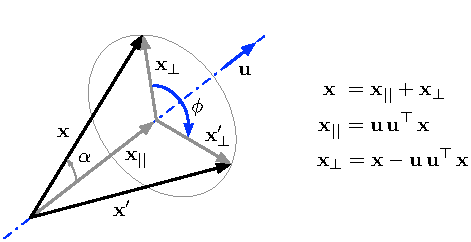
\includegraphics{figures/rotation3d}
\caption{向量 $\bfx$ 围绕轴 $\bfu$ 旋转 $\phi$ 角度,详情见正文。}
\label{fig:rotation3d}
\end{figure}

我们在 ~\figRef{fig:rotation3d} 中的旋转,遵循右手规则,说明了一个通用的 3D 向量 $\bfx$,围绕用单位向量定义的旋转轴 $\bfu$,旋转 $\phi$ 角度。 
这是通过将向量 $\bfx$ 分解成与 $\bfu$ 平行的分量 $\bfx_{||}$ ,和与 $\bfu$ 正交的分量 $\bfx_\bot$ 来完成,所以有
%
%
\begin{align*}
\bfx=\bfx_{||}+\bfx_\bot~. 
\end{align*}
%
这些部分可以很容易地计算出来 ($\alpha$ 是向量 $\bfx$ 与轴 $\bfu$ 之间的夹角),
%
%
\begin{align*}
\bfx_{||} &= \bfu \, (\norm{\bfx}\cos\alpha)  = \bfu\,\bfu\tr\,\bfx 
\\
\bfx_\bot &= \bfx - \bfx_{||} = \bfx - \bfu\,\bfu\tr\,\bfx~.
\end{align*}%
%
旋转时,平行部分不旋转, 
%
\begin{align*}
\bfx_{||}' = \bfx_{||}~,
\end{align*}
%
并且正交部分在垂直于 $\bfu$ 的平面上经历平面旋转。也就是,如果基于这个平面创建一个正交基 $\{\bfe_1,\bfe_2\}$ 
%
%
\begin{align*}
\bfe_1 &= \bfx_\bot \\
\bfe_2 &= \bfu \tcross \bfx_\bot = \bfu \tcross \bfx  ~, 
\end{align*}%
%
满足 $\norm{\bfe_1} = \norm{\bfe_2}$,则 $\bfx_\bot=\bfe_1\tdot1+\bfe_2\tdot0$。 一个 $\phi$\,rad 的旋转出现在这个平面上。
%
\begin{align*}
\bfx_\bot' = \bfe_1\cos\phi + \bfe_2\sin\phi~,
\end{align*}
%
可扩展为,
%
\begin{align*}
\bfx_\bot' = \bfx_\bot\cos\phi + (\bfu\tcross\bfx)\sin\phi~.
\end{align*}
%
将平行部分相加,得到旋转向量 $\bfx'=
\bfx'_{||}+\bfx'_\bot$~ 的表达式,即著名的向量旋转公式(\emph{vector rotation formula}),
%
\begin{align}
\eqbox{
\bfx'=
\bfx_{||}+\bfx_\bot\cos\phi+(\bfu\times\bfx)\sin\phi}~.
\label{equ:vecRotFormula}
\end{align}
%


%-------------------------------------------------------------
\subsection{旋转群 $SO(3)$}

在 $\bbR^3$ 中,旋转群 $SO(3)$ 是在组合操作下围绕原点旋转的群。旋转是保持向量长度和相对向量方向 (即,惯用手,handedness)。它在机器人学中的重要性在于,它代表了3D空间中刚体的旋转:刚体运动(\emph{rigid motion})要求在运动时精确地保持刚体内的距离、角度和相对方向 --- 否则,如果范数、角度或相对方向能不保持,则不能将机体视为刚体。

%刚体(\emph{Rigid})意味着它们维持了距离、角度和相对方向。
%不变的点不包括转换。
然后,让我们通过满足这些属性的算子定义旋转。 
一个作用于向量 $\bfv\in\bbR^3$ 的旋转算子 $r:\bbR^3\to\bbR^3; \bfv\mapsto r(\bfv)$ 可以从欧几里德空间的度量定义,由点和交叉积构成,如下所示。
%
% $SO(3)$ 群,或 $\bbR^3$ 中的旋转群,是算子 $r:\bbR^3\to\bbR^3$ 的集合,满足以下特性:
%
\begin{itemize}
%
\item 旋转保持向量范数,
%
\begin{subequations}
\begin{align}
\norm{r(\bfv)}=
\sqrt{\langle r(\bfv), r(\bfv)\rangle}=\sqrt{\langle\bfv,\bfv\rangle}\triangleq\norm{\bfv}~,\quad\forall\bfv \in\bbR^3~. \label{eq:keepnorm}
%\sqrt{r(\bfv)\tr r(\bfv)}=\sqrt{\bfv\tr\bfv}\triangleq\norm{\bfv}~,\quad\forall\bfv \in\bbR^3~. \label{eq:keepnorm}
\end{align}
%
\item 旋转保持向量之间的角度, 
%
\begin{align}
\langle r(\bfv), r(\bfw)\rangle  = \langle \bfv,\bfw\rangle = \norm{\bfv}\norm{\bfw}\cos\alpha~,\quad\forall\bfv,\bfw\in\bbR^3~.
%r(\bfv)\tr r(\bfw) = \bfv\tr\bfw = \norm{\bfv}\norm{\bfw}\cos\alpha~,\quad\forall\bfv,\bfw\in\bbR^3~.
\end{align}
\end{subequations}
%
\item 旋转保持向量的相对方向,
%
\begin{align}
\bfu\times\bfv=\bfw 
\iff 
r(\bfu)\times r(\bfv)=r(\bfw) 
~. 
\label{equ:keeporientation}
\end{align}
\end{itemize}
%
很容易证明前两个条件是等价的。因此我们可以把旋转群 $SO(3)$ 定义为,
%旋转集合作为3参数(3-vectors)向量上的算子集合有 (a) 保持范数不变,并且 (b) 维持相对方向,也就是说,
%
\begin{align}
SO(3):\{r:\bbR^3\to\bbR^3\,/\,\forall\, \bfv,\bfw\in\bbR^3~,~ \norm{r(\bfv)}=\norm{\bfv}~,~ r(\bfv)\tcross r(\bfw)=r(\bfv\tcross\bfw)\} 
~.
\end{align}
%

旋转群通常由旋转矩阵集合表示。然而,四元数也是它的一个很好的表示。 
本章的目的是证明这两种表述是同等有效的。
它们在概念上和代数上表现出许多相似之处,读者将在 \tabRef{tab:Rq} 中体会。
%
\begin{table}[htp]
\renewcommand{\arraystretch}{1.5}
\begin{center}
\caption{表示 $SO(3)$ 的旋转矩阵和四元数。}
\label{tab:Rq}
\begin{tabular}{|c|c|c|}
\hline
& 旋转矩阵, $\bfR$ & 四元数, $\bfq$ \\
\hline
\hline
参数 & $3\times3=9$ & $1+3=4$ \\
自由度(DOF) & 3 & 3 \\
约束条件 & $9-3=6$ & $4-3=1$ \\
约束条件 & $\bfR\bfR\tr=\bfI~~;~~\det(\bfR)=+1$ & $\bfq\ot\bfq^* = 1$ \\
\hline
\hline
ODE & $\dot\bfR=\bfR\hatx{\bfomega}$ & $\dot\bfq=\frac12\bfq\ot\bfomega$ \\
指数映射 & $\bfR=\exp(\hatx{\bfu\phi})$ & $\bfq=\exp(\bfu\phi/2)$ \\
对数映射 & $\log(\bfR) = \hatx{\bfu\phi}$ & $\log(\bfq) = \bfu\phi/2$ \\
与 $SO(3)$ 关系 & 单倍覆盖 & 双倍覆盖 \\
\hline
\hline
特征值 & $\bfI$ & $1$ \\
逆 & $\bfR\tr$ & $\bfq^*$ \\
组合 & $\bfR_1\,\bfR_2$  & $\bfq_1\ot\bfq_2$ \\
\hline
旋转算子 & $\bfR = \bfI + \sin\phi\hatx{\bfu} + (1-\cos\phi)\hatx{\bfu}^2$ & $\bfq = \cos\phi/2 + \bfu\sin\phi/2$ \\
旋转动作 & $\bfR\,\bfx$ & $\bfq\ot\bfx\ot\bfq^*$ \\
\hline
\multirow{3}{*}{插值} & $\bfR^t=\bfI + \sin t\phi\hatx{\bfu} \!+ (1\!-\!\cos t\phi)\hatx{\bfu}^2$ & $\bfq^t=\cos t\phi/2+\bfu\sin t\phi/2$\\
 & $\bfR_1(\bfR_1\tr\bfR_2)^t$ & $\bfq_1\ot(\bfq_1^*\ot\bfq_2)^t$ \\
 & & $\bfq_1\frac{\sin((1-t)\Delta\theta)}{\sin(\Delta\theta)}+\bfq_2\frac{\sin(t\Delta\theta)}{\sin(\Delta\theta)}$ \\
\hline
\hline
交叉关系 & \multicolumn{2}{|c|}
{$\begin{aligned}
\rule{0pt}{2.7ex} % add some vertical spacing for cosmetics
\bfR\{\bfq\} &= (q_w^2-\qv\tr\qv)\,\bfI + 2\,\qv\qv\tr + 2\,q_w\hatx{\qv} \\
\bfR\{-\bfq\}&=\bfR\{\bfq\} ~~~~~~~~~~~~~~~~~~~~\, \text{双倍覆盖} \\
\bfR\{1\}&=\bfI ~~~~~~~~~~~~~~~~~~~~~~~~~~~ \text{特征值}\\
\bfR\{\bfq^*\}&=\bfR\{\bfq\}\tr ~~~~~~~~~~~~~~~~~~~ \text{逆}\\
\bfR\{\bfq_1\ot\bfq_2\}&=\bfR\{\bfq_1\}\,\bfR\{\bfq_2\} ~~~~~~~~~~ \text{组合}\\
\bfR\{\bfq^t\} &= \bfR\{\bfq\}^t ~~~~~~~~~~~~~~~~~~~\, \text{插值} 
\end{aligned}$} \\
\hline
\end{tabular}
\end{center}
\end{table}%
%
或许,最重要的区别在于,单位四元数组构成了 $SO(3)$ 双倍覆盖(因此技术上不是 $SO(3)$ 本身),这在我们的大多数应用中并不重要。\footnote{在旋转空间进行插值时,需要考虑双倍覆盖的效果。这个很容易,我们将在 \secRef{sec:slerp} 看到细节。}
为了快速比较和评估,该表是预先插入的。
接下来的章节将探讨 $SO(3)$ 的旋转矩阵和四元数表示。



\subsection{旋转群和旋转矩阵}

%The name $SO(3)$ is explained by the fact that it can be represented by the set of \emph{Special Orthogonal} $3\times3$ matrices, otherwise called \emph{proper orthogonal} matrices, as we explore in this section. 

算子 $r()$ 是线性的,因为它是由线性的标量和向量乘积定义的。 
因此,它可以用矩阵 $\bfR\in\bbR^{3\times3}$来表示,该矩阵在矩阵乘积上对向量 $\bfv\in\bbR^3$ 产生旋转,
%
\begin{align}
r(\bfv) = \bfR\,\bfv~.
\end{align}
%
将其注入方程 \eqRef{eq:keepnorm} ,使用点积 $\langle\bfa,\bfb\rangle=\bfa\tr\bfb$ 和扩展,我们对所有的 $\bfv$ 有,
%
\begin{align}
(\bfR\bfv)\tr(\bfR\bfv) = \bfv\tr\bfR\tr\bfR\bfv = \bfv\tr\bfv
~,
\end{align}
%
得到 $\bfR$ 上的正交(\emph{orthogonality})条件,
%
\begin{align}
\eqbox{
\bfR\tr\bfR = \bfI = \bfR\,\bfR\tr
}
~. 
\label{equ:Rorthogonal}
\end{align}
%
上面的条件确实是正交的条件,因为我们可以从中观察到,通过写 $\bfR=[\bfr_1,\bfr_2,\bfr_3]$ 并代入上面, $\bfR$ 的列向量 $\bfr_i$ ,其中 $i\in\{1,2,3\}$, 是单位长度且相互正交,
%
\begin{align*}
\langle\bfr_i,\bfr_i\rangle &= \bfr_i\tr\bfr_i = 1 \\%~,\quad \textrm{if } i = j \\
\langle\bfr_i,\bfr_j\rangle &= \bfr_i\tr\bfr_j = 0 ~,\quad \textrm{if } i\neq j~.
\end{align*}
%
由于这个原因,保持向量范数和角度的变换集合被称为正交群(\emph{Orthogonal group}),表示为 $O(3)$。
正交群包括旋转 (刚体运动) 和反射 (非刚体运动)。
这里的群(\emph{group})的概念实质上 (和非正式地) 意味着两个正交矩阵的乘积总是一个正交矩阵,%
\footnote{\label{ftn:O3}%
让 $\bfQ_1$ 和 $\bfQ_2$ 正交,
并且构建 $\bfQ=\bfQ_1\,\bfQ_2$ 。
则 $\bfQ\tr\bfQ=
\bfQ_2\tr\bfQ_1\tr\bfQ_1\bfQ_2=\bfQ_2\tr\bfI\bfQ_2=\bfI$ 。}
并且每个正交矩阵允许一个逆。
实际上,正交条件方程 \eqRef{equ:Rorthogonal} 意味着利用转置矩阵实现逆旋转,
%
\begin{align}
\bfR\inv=\bfR\tr~.
\end{align}


添加相对方向条件方程 \eqRef{equ:keeporientation} 可确保刚体运动 (从而丢弃反射运动),并且其结果对 $\bfR$ 产生一个附加约束%
\footnote{注意反射运动满足 $|\bfR|=\det(\bfR)=-1$,并且不构成群,因为 $|\bfR_1\bfR_2|=1\neq-1$ 。}
%
\begin{align}\label{equ:unitDet}
\eqbox{
\det(\bfR)=1
}
~.
\end{align}
%
%
具有正单位行列式的正交矩阵通常被称为真(\emph{proper})矩阵或特殊(\emph{special})矩阵。这类特殊正交矩阵(\emph{special orthogonal matrices})的集合被称为特殊正交群(\emph{Special Orthogonal group})$SO(3)$ ,是 $O(3)$ 的一个子群。
作为一个群,两个旋转矩阵的乘积总是一个旋转矩阵。%
\footnote{%
参见脚注 \ref{ftn:O3} 对于 $O(3)$ 并且对 $SO(3)$ 附加这个条件:让 $|\bfR_1|=|\bfR_2|=1$,则 $|\bfR_1\bfR_2|=|\bfR_1|\,|\bfR_2|=1$。}




\subsubsection{指数映射}

指数映射 (和对数映射,我们在下一节中看到) 是一个强大的数学工具,可以轻松而精确地在旋转的 3D 空间中工作。它表示了适合旋转空间的微积分语料库的入口。指数映射允许我们正确定义导数、扰动和速度,并对它们进行操作。因此,它在旋转或方向空间中的估计问题中是必要的。

旋转构成刚性运动。这种刚性意味着可以在 $SO(3)$ 中定义一个连续的轨迹或路径(\emph{path}), $r(t)$,该轨迹或路径连续地将刚体从其初始方向,$r(0)$,旋转到其当前方向, $r(t)$。
由于变换是连续的,因此研究这种变换的时间导数是合理的。
我们通过推导我们刚刚看到的性质方程 \eqRef{equ:Rorthogonal} 和 \eqRef{equ:unitDet} 来实现推导。

%We explore here the case of the rotation matrix representation $\bfR(t)$, as follows.
首先,我们注意到不可能在满足连续逃逸单位行列式条件方程 ~\eqRef{equ:unitDet} 的同时,满足方程 ~\eqRef{equ:Rorthogonal} ,因为这意味着行列式从 $+1$ 跳到 $-1$。\footnote{换而言之:旋转不能通过连续变换成为反射。}
因此我们只需要研究正交条件方程 \eqRef{equ:Rorthogonal} 。上面写着
%
\begin{align}
\dif{}{t}{(\bfR\tr\bfR)} = \dot\bfR\tr\bfR+\bfR\tr\dot\bfR = 0
~,
\end{align}
%
其结果为
%
\begin{align}
\bfR\tr\dot\bfR 
= -(\bfR\tr\dot\bfR)\tr
~,
\end{align}
%
这意味着矩阵 $\bfR\tr\dot\bfR$ 是一个斜对称矩阵 (即,它等于其转置的负数)。 
将 $3\times3$ 的斜对称矩阵集合表示为 $\so(3)$,并得到 $SO(3)$ 的李代数(\emph{Lie algebra})的名称。
斜对称 $3\times3$ 矩阵的形式是,
%These matrices have 3\,DOF, and it is convenient to write them as the cross-product matrix,
%
\begin{align}
\hatx{\bfomega} \triangleq \begin{bmatrix}
0 & -\omega_z & \omega_y \\
\omega_z & 0 & -\omega_x \\
-\omega_y & \omega_x & 0
\end{bmatrix}
~;
\end{align}
%
它们有3个自由度(3\,DOF),并对应于交叉积矩阵,如我们已经在方程 \eqRef{equ:skew} 所介绍的。这就建立了一个一对一映射 $\bfomega\in\bbR^3\leftrightarrow\hatx{\bfomega}\in\so(3)$.
%
%Because $\so(3)$ is the space where the derivatives of $r(t)$ live, it constitutes the \emph{tangent space} to $SO(3)$, or the \emph{velocity space}, also known as its \emph{Lie algebra}.
让我们取一个向量 $\bfomega=(\omega_x,\omega_y,\omega_z)\in\bfR^3$ 并且写
%
\begin{align}
\bfR\tr\dot\bfR = \hatx{\bfomega}
~.
\end{align}
%
%and let us call $\bfomega$ the vector of instantaneous angular velocities. 
这就产生了常微分方程 (ODE),
%
\begin{align}
\label{equ:Rdot}
\dot\bfR=\bfR\hatx{\bfomega}~.
\end{align}
%
在原点附近,我们有 $\bfR=\bfI$ 则上面的方程降为 $\dot\bfR=\hatx{\bfomega}$。
因此,我们可以将李代数 $\so(3)$ 解释为原点处 $r(t)$ 导数的空间;
%Because $\so(3)$ is the space where the derivatives of $r(t)$ live, 
它构成了对 $SO(3)$ 的切空间(\emph{tangent space})或速度空间(\emph{velocity space})。
根据这些事实,我们可以很好地称 $\bfomega$ 为瞬时角速度向量。 

如果 $\bfomega$ 是常数,上面的微分方程可以用时间积分为
%
\begin{align}
\bfR(t) = \bfR(0)\,e^{\hatx{\bfomega}t} = \bfR(0)\,e^{\hatx{\bfomega t}} 
\end{align}
%
其中指数 $e^{\hatx{x}}$ 由它的泰勒级数定义,如我们在下一节中看到的。
因为 $\bfR(0)$ 和 $\bfR(t)$ ,那么显然 $e^{\hatx{\bfomega t}}=\bfR(0)\tr\bfR(t)$ 是旋转矩阵。
定义向量 $\bfphi\triangleq\bfomega\Dt$ 为在 $\Dt$ 周期内完全编码旋转的旋转向量,我们得到
%
\begin{align}
\eqbox{
\bfR = e^{\hatx{\bfphi}} \label{equ:vectomat}
}~.
\end{align}
%
这就是所谓的指数映射,是从 $\so(3)$ 到 $SO(3)$ 的应用,
%
\begin{align}
\exp: \so(3) \to SO(3) ~;~ \hatx{\bfphi} \mapsto \exp(\hatx{\bfphi})=e^{\hatx{\bfphi}}
~.
\end{align}
%

\subsubsection{大写的指数映射}

上面的指数映射有时会滥用一些符号表示,即 $\bfphi\in\bbR^3$ 和 $\hatx{\bfphi}\in\so(3)$ 混淆.
%
为了避免可能的歧义,我们选择用大写 $\Exp$ 的显式表示法写这个新的应用 $\bbR^3\to SO(3)$ ,得到 (参见 \figRef{fig:exp_map_R})
%
\begin{figure}[tb]
\begin{center}
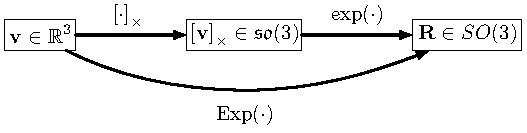
\includegraphics{figures/exp_map_R}
\caption{旋转矩阵的指数映射。}
\label{fig:exp_map_R}
\end{center}
\end{figure}
%
\begin{align}
\Exp: \bbR^3 \to SO(3) ~;~ \bfphi \mapsto \Exp(\bfphi) = e^{\hatx{\bfphi}}
~.
\end{align}
%
它与指数映射的关系是平凡的,
%
\begin{align}
\Exp(\bfphi) \triangleq \exp(\hatx{\bfphi})
~.
\end{align}


在下面的部分中,我们将看到向量 $\bfphi$,称为旋转向量或角-轴(angle-axis)向量,通过 $\bfphi=\bfomega\Dt=\phi\bfu$ 编码旋转的角度 $\phi$ 和轴 $\bfu$ 。


%-------------------------------------------------------------
\subsubsection{旋转矩阵和旋转向量: Rodrigues 旋转公式}
%\subsubsection{}


旋转矩阵由旋转向量 $\bfphi=\phi\bfu$ 通过指数映射方程 \eqRef{equ:vectomat} 定义,
同时交叉积矩阵 $\hatx{\bfphi}=\phi\hatx{\bfu}$ 如方程 \eqRef{equ:skew} 中定义。
方程 \eqRef{equ:vectomat} 的泰勒展开式,用 $\bfphi=\phi\bfu$ 读到, 
%
\begin{align}
\bfR=e^{\phi\hatx{\bfu}} = 
	  \bfI 
	+ 			\phi\hatx{\bfu} 
	+ \frac12	\phi^2\hatx{\bfu}^2
	+ \frac1{3!}\phi^3\hatx{\bfu}^3 
	+ \frac1{4!}\phi^4\hatx{\bfu}^4 
	+ \dots
\end{align}
%
当应用于单位向量, $\bfu$,矩阵 $\hatx{\bfu}$ 满足
%
%
\begin{align}
\hatx{\bfu}^2 &= \bfu\bfu\tr-\bfI
\label{equ:prop1}
\\
\hatx{\bfu}^3 &= -\hatx{\bfu}
~, \label{equ:prop2}
\end{align}%
%
并且因此 $\hatx{\bfu}$ 的所有幂可以用循环模式中的 $\hatx{\bfu}$ 和 $\hatx{\bfu}^2$ 来表示,
%
\begin{align}
\hatx{\bfu}^4 &= -\hatx{\bfu}^2 
& \hatx{\bfu}^5 &= \hatx{\bfu} 
& \hatx{\bfu}^6 &= \hatx{\bfu}^2 
& \hatx{\bfu}^7 &=-\hatx{\bfu} 
~~\cdots 
~.
\end{align}
%
然后,根据 $\hatx{\bfu}$ 和 $\hatx{\bfu}^2$,对泰勒级数进行分组,分别识别出 $\sin\phi$ 和 $\cos\phi$的级数,得到一个从旋转向量得到旋转矩阵的闭合形式,即所谓的Rodrigues旋转公式(\emph{Rodrigues rotation formula}),
%
\begin{align}
\eqbox{
\bfR %= e^{\hatx{\bfphi}} 
= \bfI + \sin\phi\hatx{\bfu} + (1-\cos\phi)\hatx{\bfu}^2
}~, \label{equ:rodrigues}
\end{align}%
%
其中我们表示 $\bfR\{\bfphi\}\triangleq\Exp(\bfphi)$ 。
这个公式允许一些变体,例如,使用方程 \eqRef{equ:prop1} ,
%
\begin{align}
\bfR &= \bfI\cos\phi + \hatx{\bfu}\sin\phi + \bfu\bfu\tr(1-\cos\phi)
~.
\end{align}%

\subsubsection{对数映射}

我们把对数映射定义为指数映射的逆,
%
\begin{align}
\log : SO(3)\to\so(3)~;~ \bfR \mapsto \log(\bfR)=\hatx{\bfu\,\phi}
~,
\end{align}
%
其中
%
\begin{align}
\phi &= \arccos\left(\frac{\trace(\bfR)-1}{2}\right) 
\\
\bfu &= \frac{(\bfR-\bfR\tr)^\vee}{2\sin\phi} 
~,
\end{align}
%
其中 $\bullet^\vee$ 是 $\hatx{\bullet}$的倒数,即, $(\hatx{\bfv})^\vee=\bfv$ 和 $\hatx{\bfV^\vee}=\bfV$ 。

我们还定义了一个大写版本 $\Log$,它允许我们从旋转矩阵中直接恢复旋转向量 $\bfphi=\bfu\phi\in\bbR^3$ , 
%
\begin{subequations}
\begin{align}
\Log: SO(3) \to \bbR^3 ~;~ \bfR\mapsto\Log(\bfR) = \bfu\,\phi 
~.
\end{align}
\end{subequations}
%
它与对数映射的关系是平凡的,
%
\begin{align}
\Log(\bfR) \triangleq (\log(\bfR))^\vee
~.
\end{align}



\subsubsection{旋转动作}

旋转一个向量 $\bfx$ 围绕单位轴 $\bfu$ 转过一个角度 $\phi$ %following the right-hand rule 
要用线性乘积来执行
%
\begin{align}
\bfx'=\bfR\,\bfx
~, 
\label{equ:rotWithMat}
\end{align}
%
其中 $\bfR=\Exp(\bfu\phi)$ 。
这可以通过扩展方程 \eqRef{equ:rotWithMat} ,
使用方程 \eqRef{equ:rodrigues} , \eqRef{equ:prop1}  和 \eqRef{equ:prop2} 来表示,
%in a way akin to the last steps of \eqRef{equ:quatRotFormula}, 
%to obtain the vector rotation formula \eqRef{equ:vecRotFormula},
%
\begin{align}
\begin{split}
\bfx' &= \bfR\,\bfx  \\
&= (\bfI + \sin\phi\hatx{\bfu} + (1-\cos\phi)\hatx{\bfu}^2)\,\bfx  \\
&= \bfx + \sin\phi\hatx{\bfu}\bfx + (1-\cos\phi)\hatx{\bfu}^2\bfx  \\
&= \bfx + \sin\phi(\bfu\tcross\bfx) + (1-\cos\phi)(\bfu\bfu\tr-\bfI)\,\bfx  \\
&= \bfx_\| + \bfx_\bot + \sin\phi(\bfu\tcross\bfx) - (1-\cos\phi)\,\bfx_\bot  \\
&= \bfx_\| + (\bfu\tcross\bfx)\sin\phi + \bfx_\bot\cos\phi
~,
\end{split}
\end{align}%
%
这正是向量旋转公式 \eqRef{equ:vecRotFormula} ,


%-------------------------------------------------------------
\subsection{旋转群和四元数}

为了教学的目的,我们有兴趣强调四元数和旋转矩阵之间的联系,作为旋转群 $SO(3)$的表示。 
为此,四元数旋转动作的众所周知的公式是,
%For this, it will be convenient to assume as hypothesis that the rotation action using quaternions is achieved with the double product,
%
\begin{align} \label{equ:qrot}
r(\bfv)=\bfq\ot\bfv\ot\bfq^*
~,
\end{align}
%
这里是最初的假设。
这使我们能够发展出完整的四元数部分,其中包含一个追溯我们用于旋转矩阵的部分的论述。 
这一假设的正确性将在稍后的,在 \secRef{sec:qRotAction} 中得到证明,从而验证该方法。 
%This enables us to position the unit quaternion as a powerful representation of the rotation group $SO(3)$.

然后,我们将上述旋转注入正交条件方程 \eqRef{eq:keepnorm} ,并使用方程 \eqRef{equ:norm_prod} 做为
%
\begin{align}
\norm{\bfq\ot\bfv\ot\bfq^*}=\norm{\bfq}^2\norm{\bfv} = \norm{\bfv}
~.
\end{align}
%
这就得到 $\norm{\bfq}^2=1$,这就是四元数的单位范数条件,它是,
%
\begin{align} \label{equ:q_unit}
\eqbox{
\bfq^*\ot\bfq = 1 = \bfq\ot\bfq^*
}
~.
\end{align}
%
这个条件类似于我们在旋转矩阵中遇到的条件,参见方程 \eqRef{equ:Rorthogonal} ,它读为 $\bfR\tr\bfR=\bfI=\bfR\bfR\tr$。我们建议读者暂停一会讨论它们的相似之处。

%
类似地,我们证明相对方向条件方程 \eqRef{equ:keeporientation} 通过构造(我们使用方程 \eqRef{equ:quatCommutatorPure} 两次,如下所示)得到满足,
%
\begin{align}
\begin{split}
r(\bfv)\times r(\bfw) 
&= (\bfq\ot\bfv\ot\bfq^*) \times (\bfq\ot\bfw\ot\bfq^*) \\
%
\eqRef{equ:quatCommutatorPure}~~
&= \frac12\big((\bfq\ot\bfv\ot\bfq^*) \ot (\bfq\ot\bfw\ot\bfq^*) - (\bfq\ot\bfw\ot\bfq^*) \ot (\bfq\ot\bfv\ot\bfq^*) \big) \\
&= \frac12(\bfq\ot\bfv\ot\bfw\ot\bfq^* - \bfq\ot\bfw\ot\bfv\ot\bfq^*) \\
&= \frac12(\bfq\ot(\bfv\ot\bfw - \bfw\ot\bfv)\ot\bfq^*) \\
%
\eqRef{equ:quatCommutatorPure}~~
&= \bfq\ot(\bfv\times\bfw)\ot\bfq^* \\
&= r(\bfv\times\bfw)
~.
\end{split}
\end{align}


单位四元数的集合在乘法操作下构成一个群。这个群在拓扑上是一个 3-sphere,即 $\bbR^4$ 的单位球的 3D 表面,通常称为 $S^3$ 。
%The group $S^3$ constitutes a double cover of $SO(3)$.
%Since $\bfq$ and $-\bfq$ produce the same rotation, see \eqRef{equ:qrot}, we have that $S^3$ is a double cover of $SO(3)$.

\subsubsection{指数映射}

让我们考虑一个单位四元数 $\bfq\in S^3$ ,就是, $\bfq^*\ot\bfq=1$ ,并让我们继续处理,就像我们对旋转矩阵 $\bfR\tr\bfR=\bfI$ 的正交性条件所做的那样。
取时间导数,
%
\begin{align}
\dif{(\bfq^*\ot\bfq)}{t} = \dot\bfq^*\ot\bfq+\bfq^*\ot\dot\bfq=0
~,
\end{align}
%
由此可见
%
\begin{align}
\bfq^*\ot\dot\bfq = -(\dot\bfq^*\ot\bfq) = -(\bfq^*\ot\dot\bfq)^*~,
\end{align}
%
这意味着 $\bfq^*\ot\dot\bfq$ 是一个纯四元数 (即,它等于它的负共轭,因此它的实部为零)。
%In the quaternion case, however, this space is not directly the velocity space, but rather the space of the half-velocities, as we will se soon.
%The set of pure quaternions is denoted $\bbH_p=\Im(\bbH)$ and constitutes the Lie Algebra of $\bbH$.
因此我们得到一个纯四元数 $\bfOmega\in\bbH_p$ 并写为,
%
\begin{align}
\bfq^*\ot\dot\bfq = \bfOmega = \begin{bmatrix}
0\\\bfOmega
\end{bmatrix} 
\in\bbH_p
~.
\end{align}
%
左乘 $\bfq$ 得到微分方程,
%
\begin{align}
\label{equ:qdotOmega}
\dot\bfq = \bfq\ot\bfOmega~.
\end{align}
% 
在原点附近,我们有 $\bfq=1$ 则上面的方程降为 $\dot\bfq=\bfOmega\in\bbH_p$ 。
因此,纯四元数空间 $\bbH_p$ 构成四元数的单位球面 $S^3$ 的切空间(\emph{tangent space})或李代数(Lie Algebra)。 
%In the quaternion case, vectors in the tangent space correspond to the half of the angular velocity vectors.
然而,在四元数的情况下,这个空间并不直接是速度空间,而是一半速度的空间,我们很快就会看到。


如果 $\bfOmega$ 是常数,微分方程可以积分为
%
\begin{align}\label{equ:qexpWt}
\bfq(t) = \bfq(0)\ot e^{\bfOmega\, t}
~,
\end{align}
%
其中,因为 $\bfq(0)$ 和 $\bfq(t)$ 是单位四元数,所以指数 $e^{\bfOmega t}$ 也是单位四元数 --- 这是我们从四元数指数方程 ~\eqRef{equ:EulerFormulaQuat} 中已经知道的。
%
定义 $\bfV\triangleq\bfOmega\Dt$ 我们有
%
\begin{align}\label{equ:qexpV}
\eqbox{
\bfq = e^{\bfV}
}~.
\end{align}
%
这又是一个指数映射:从纯四元数空间到单位四元数表示的旋转空间的应用,
%
\begin{align}\label{equ:q_expmap}
\exp:\bbH_p\to S^3~;~ \bfV\mapsto \exp(\bfV) = e^{\bfV}
\end{align}
%

\subsubsection{大写指数映射}

%At this point, we still have to relate the pure quaternion $\bfV$ in the exponential map~\eqRef{equ:q_expmap} with the angle-axis rotation parameters in Cartesian space. 
我们将看到,纯四元数 $\bfV$ 在指数映射方程 ~\eqRef{equ:q_expmap} 中的编码,通过 $\bfV=\theta\bfu = \phi\bfu/2$,旋转轴 $\bfu$ 和旋转角的一半, $\theta=\phi/2$,来进行。
我们将很快对这个一半角度的事实提供充分的解释,主要在第 \ref{sec:qRotAction}, \ref{sec:double_cover} 和 \ref{sec:isoclinic} 节。现在,可以说,由于旋转动作是由双倍乘积 $\bfx'=\bfq\ot\bfx\ot\bfq^*$ 完成的,向量 $\bfx$ 经历的旋转是 $\bfq$中编码的旋转的“两倍”,或者等价地说,四元数 $\bfq$ 编码 ~$\bfx$上的“一半”旋转。

为了表达角-轴(angle-axis)旋转参数, $\bfphi=\phi\bfu\in\bbR^3$,和四元数之间的直接关系,我们定义指数映射的一个大写版本,它捕获半角效应 (参见 \figRef{fig:exp_map_q}),
%
\begin{figure}[tb]
\begin{center}
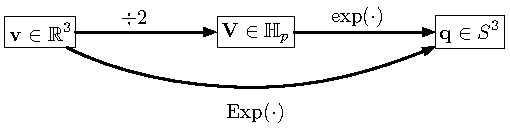
\includegraphics{figures/exp_map_q}
\caption{四元数的指数映射。}
\label{fig:exp_map_q}
\end{center}
\end{figure}
%
\begin{align}
\Exp:\bfR^3\to S^3~;~\bfphi\mapsto\Exp(\bfphi)=e^{\bfphi/2}
\end{align}
%
它与指数映射的关系是平凡的,
%
\begin{align}
\Exp(\bfphi) \triangleq \exp(\bfphi/2)
~.
\end{align}


这也方便引入角速度向量 $\bfomega=2\bfOmega\in\bbR^3$,使得方程 \eqRef{equ:qdotOmega} 和 \eqRef{equ:qexpWt} 变成,
%
\begin{align}
\dot\bfq &= \frac12\bfq\ot\bfomega \label{equ:qdot} \\ 
\bfq &= e^{\bfomega t/2}
~.
\end{align}
%%
%where we call $\bfomega$ the vector of instantaneous angular velocities ---the presence of the `half' term will become clear in the following sections, especially in Sections \ref{sec:quatAndVector} and \ref{sec:isoclinic}.
%Left-multiplication by $\bfq$ yields the differential equation,
%%
%\begin{align}
%\label{equ:qdot}
%\dot\bfq = \frac12\,\bfq\ot\bfomega~.
%\end{align}
%% 
%If $\bfomega$ is constant, this can be integrated as
%%
%\begin{align}
%\bfq(t) = \bfq(0)\ot e^{\bfomega t/2}
%~,
%\end{align}
%%
%where, since $\bfq(0)$ and $\bfq(t)$ are unit quaternions, the exponential $e^{\bfomega t/2}$ is also a unit quaternion ---something we already knew from the properties of the quaternion exponential.
%%
%Defining the vector $\bfphi\triangleq\bfomega\Dt$ as the angle-axis vector encoding the full rotation over a period $\Dt$, we have
%%
%\begin{align}\label{equ:vectoquatEuler}
%\eqbox{
%\bfq = e^{\bfphi/2}
%}~.
%\end{align}
%
%This is again an exponential map, from the space of pure quaternions to the space of unit quaternions.
%%
%As we did for the exponential map of the rotation matrix, we opt for an explicit notation using a capitalized $\Exp$ function, which relates directly the rotation vector to the quaternion,
%%
%\begin{align}
%\Exp: \bbR^3 \to \bbH ~;~  \bfphi \mapsto \Exp(\bfphi) = e^{\bfphi/2} 
%~.
%\end{align}
%%
%Its relation with the quaternion exponential is trivial,
%%
%\begin{align}
%\Exp(\bfphi) \triangleq \exp(\bfphi/2)
%~.
%\end{align}


%-------------------------------------------------------------
\subsubsection{四元数和旋转向量}
\label{sec:quatAndVector}

设 $\bfphi=\phi\bfu$ 是一个旋转向量表示绕着轴 $\bfu$ 的 $\phi$\,rad 的旋转,
然后,
指数映射可以使用Euler公式(\emph{Euler formula})进行扩展(对于一个完整的扩展参见方程 \eqsRef{equ:qvPowers}{equ:EulerFormulaQuat}),
%
\begin{align}
\eqbox{
\bfq \triangleq \Exp(\phi\bfu) = e^{\phi\bfu/2} = \cos \frac{\phi}{2} + \bfu\sin\frac{\phi}{2}=\begin{bmatrix}
\cos(\phi/2) \\
\bfu\sin(\phi/2)
\end{bmatrix}
}
~.   \label{equ:vectoquat}
\end{align}
%
我们称之为旋转向量到四元数(\emph{rotation vector to quaternion})的转换公式,并且在本文中标记为 
$\bfq=\bfq\{\bfphi\}\triangleq\Exp(\bfphi)$. 




\subsubsection{对数映射}

我们把对数映射定义为指数映射的逆,
%
\begin{align}
\log:S^3\to\bbH_p ~;~ \bfq\mapsto \log(\bfq) = \bfu\theta
~,
\end{align}
%
这当然是我们在 \secRef{sec:qlog} 中给出的四元数对数的定义。
我们还定义了大写的对数映射,在笛卡尔 3-space 中,它直接提供了旋转的角度 $\phi$ 和轴,
%
\begin{align}
\Log:S^3\to\bbR^3 ~;~ \bfq\mapsto \Log(\bfq) = \bfu\phi
~.
\end{align}
%
它与对数映射的关系是平凡的,
%
\begin{align}
\Log (\bfq) \triangleq 2\log(\bfq)
~.
\end{align}
%

对于它的实现,我们使用 $\arctan(y,x)$的四象限版本。
从方程 \eqRef{equ:vectoquat} 中,
%
\begin{subequations}
\begin{align}
\phi &= 2\arctan(\norm{\qv},q_w) \\
\bfu &= \qv / \norm{\qv} \label{equ:qvec}
~.
\end{align}
\end{subequations}
%
对于小角度四元数,方程 \eqRef{equ:qvec} 发散。于是我们对 $\arctan()$ 函数使用泰勒级数并截断,得到,
%
\begin{equation}
\Log(\bfq) = \theta\bfu 
\approx 2\,\frac{\qv}{q_w} \left(1 - \frac{\norm{\qv}^2}{3q_w^2}\right) \label{equ:log_q_small}
~.
\end{equation}


\subsubsection{旋转动作}
\label{sec:qRotAction}

我们终于在这里证明用四元数旋转向量的假设方程 ~\eqRef{equ:qrot} ,  
%$\bfx'=\bfq\otimes\bfx\otimes\bfq^*$, 
从而验证到目前为止所有的资料。
%, and stating the unit quaternion $\bfq$ as a proper representation of the rotation group $SO(3)$.
%
用双四元数乘积,也称为“三明治”乘积来执行一个向量 $\bfx$ 绕轴 $\bfu$ 旋转一个角度 $\phi$ 这个动作,
%
\begin{align}
\bfx' = \bfq\otimes\bfx\otimes\bfq^* ~, \label{equ:sandwichProd}
\end{align}
%
式中 $\bfq=\Exp(\bfu\phi)$,并且
其中向量 $\bfx$ 已经写为四元数形式,就是 
%
\begin{align}
\bfx= x i + y j + z k = \begin{bmatrix}
0 \\ \bfx
\end{bmatrix} \in \bbH_p
~. \label{equ:quatvec}
\end{align}%
%
%
为了证明这个双乘积确实执行了所需的向量旋转,我们使用方程 \eqRef{equ:quatProdVec} ,
\eqRef{equ:vectoquat},和基本向量和三角恒等式来扩展方程 ~\eqRef{equ:sandwichProd} 如下,
%
\begin{align}\label{equ:quatRotFormula}
\begin{split}
\bfx'
&= \bfq \ot \bfx \ot \bfq^* \\
&= \Big(\cos \frac{\phi}{2} + \bfu \sin \frac{\phi}{2}\Big)
 \ot (0+\bfx)
 \ot \Big(\cos \frac{\phi}{2} - \bfu \sin \frac{\phi}{2}\Big)
 \\
&= \bfx \cos^2 \frac{\phi}{2} + (\bfu\ot\bfx - \bfx\ot\bfu) \sin \frac{\phi}{2} \cos \frac{\phi}{2} - \bfu\ot\bfx\ot\bfu \sin^2 \frac{\phi}{2} \\
&= \bfx \cos^2 \frac{\phi}{2} + 2 (\bfu \tcross \bfx) \sin \frac{\phi}{2} \cos \frac{\phi}{2} - (\bfx (\bfu \tr \bfu) - 2 \bfu (\bfu \tr \bfx)) \sin^2 \frac{\phi}{2} \\
&= \bfx (\cos^2 \frac{\phi}{2} - \sin^2 \frac{\phi}{2}) + (\bfu \tcross \bfx) (2\sin\frac{\phi}{2} \cos\frac{\phi}{2}) + \bfu (\bfu \tr \bfx) (2\sin^2 \frac{\phi}{2}) \\
&= \bfx \cos \phi + (\bfu \tcross \bfx) \sin \phi + \bfu (\bfu \tr \bfx) (1 - \cos \phi) \\
&= (\bfx - \bfu \,\bfu \tr \bfx) \cos \phi + (\bfu \tcross \bfx) \sin \phi + \bfu \,\bfu \tr \bfx \\
&= \bfx_{\bot} \cos \phi + (\bfu \tcross \bfx) \sin \phi + \bfx_{||} ~,
\end{split}
\end{align}%
%
这正是向量旋转公式 ~\eqRef{equ:vecRotFormula} 。


\subsubsection{ $SO(3)$ 流形的双倍覆盖。}
\label{sec:double_cover}

考虑一个单位四元数 $\bfq$。当其被视为一个规则的 4-vector时, $\bfq$ 和特征四元数 $\bfq_1=[1,0,0,0]$ 之间的角度 $\theta$ 表示方向的原始值,
%
\begin{align}
\cos\theta = \bfq_1\tr\bfq = \bfq(1) = q_w
~.
\end{align}
%
同时,在 3D 空间中被四元数 $\bfq$ 旋转的物体的旋转角 $\phi$ 满足
%
\begin{align}
%\bfq_1^*\ot\bfq = 
\bfq = \begin{bmatrix}
q_w \\ \qv
\end{bmatrix} = \begin{bmatrix}
\cos\phi/2 \\ \bfu\sin\phi/2
\end{bmatrix}
~.
\end{align}
%
也就是说,我们有 $q_w = \cos\theta = \cos\phi/2$,
所以四元数向量和 4D 空间中的特征值之间的夹角是 3D 空间中四元数旋转的夹角的一半,
%
\begin{align}
\theta = \phi/2
~.
\end{align}

我们在 \figRef{fig:double_cover} 中演示了这个双倍覆盖。
当两个四元数向量之间的夹角是 $\theta=\pi/2$ 时, 3D 旋转已经到达 $\phi=\pi$,这是半圈。 
当四元数向量旋转半圈时, $\theta=\pi$ , 3D 旋转已经完成了一个完整的旋转。 
%This is in accordance with a previous result showing that the negated quaternion represents the same orientation. 
四元数向量的第二个半圈, $\pi<\theta<2\pi$,表示 3D 旋转的第二个全圈 $2\pi<\phi<4\pi$,这就是旋转流形的第二个覆盖。

\begin{figure}[htbp]
\begin{center}
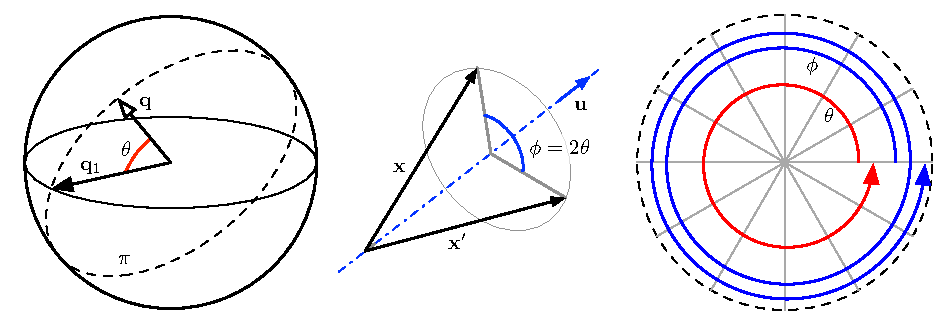
\includegraphics{figures/double_cover}
\caption{旋转流形的双倍覆盖。左边:四元数 $\bfq$ 在单位 3-sphere 中用单位四元数 $\bfq_1$ 定义一个角度 $\theta$ 。中间: 3D 旋转的结果 $\bfx'=\bfq\ot\bfx\ot\bfq^*$ 比原来的四元数有双倍的角度 $\phi$ 。右边: 将 4D 和 3D 旋转平面叠加,观察四元数 $\bfq$ 在 3-sphere 上的一圈(红色)如何表示 3D 空间中被旋转向量 $\bfx$ 的两圈 (蓝色)。}
\label{fig:double_cover}
\end{center}
\end{figure}


%\subsubsection{The quaternion as a representation of $SO(3)$}




%-------------------------------------------------------------
\subsection{旋转矩阵和四元数}

正如我们刚才看到的,给定一个旋转向量 $\bfphi=\bfu\,\phi$,对于单位四元数和旋转矩阵的指数映射产生旋转算子 
$\bfq=\Exp(\bfu\,\phi)$ 
和
$\bfR=\Exp(\bfu\,\phi)$ 
这旋转向量 $\bfx$ 实际上围绕着相同的 $\bfu$ 有着相同的角度 $\phi$ 。% 
%
\footnote{指数映射 $\bfR=\Exp(\bfphi)$ 和 $\bfq = \Exp(\bfphi)$ 之间明显的符号歧义性很容易由上下文解决:
在某些情况下,它只是返回值的类型, $\bfR$ 或 $\bfq$; 
其它情况下是四元数乘积 $\ot$ 存在或不存在。}
即,如果
%
\begin{align}
\forall \bfphi,\bfx \in \bbR^3,~ 
\bfq = \Exp(\bfphi) 
,~ 
\bfR=\Exp(\bfphi)
%\rightarrow 
%\bfq\ot%\ol
%\bfx\ot\bfq^* = \bfR\,\bfx ~,
\end{align}
%
%or, seen side by side,
%%
%\begin{align*}
%%\ol
%\bfx' &= \bfq\otimes
%%\ol
%\bfx\otimes\bfq^* ~,
%& 
%\bfx' &= \bfR\,\bfx~.
%\end{align*}%
%
%Here, we used the bar notation $\ol\bfx$ to indicate that the vector $\bfx$ in the left equation is expressed in quaternion form~\eqRef{equ:quatvec}, thus differentiating it from that on the right. 
%However, this circumstance is mostly unambiguous and can be derived from the context, and especially by the presence of the quaternion product $\otimes$. 
%In what is to follow, we are omitting this bar and writing simply,
%%
%$\bfx' = \bfq\otimes\bfx\otimes\bfq^*$\,.
%
%This allows us to 
%write,%
%\footnote{More explicit expressions would be,~ 
%$\bfq\otimes\ol\bfx
%\otimes\bfq^* = \ol{ \bfR\bfx
%}$~,
%~or~ 
%$\bfq\otimes\begin{bmatrix}
%0\\\bfx
%\end{bmatrix}\otimes\bfq^* = \begin{bmatrix}
%0 \\ \bfR\bfx
%\end{bmatrix}$~. See \secRef{sec:altQuat}.
%}
%
那么,
%
\begin{align}
\bfq\otimes\bfx\otimes\bfq^* = \bfR\,\bfx~.
\end{align}
%
由于这个恒等式的两边在 $\bfx$中是线性的,所以通过展开左边和识别右边的项,找到了与四元数等价的旋转矩阵的表达式,从而得到四元数到旋转矩阵(\emph{quaternion to rotation matrix})公式,
%
\begin{align}
\eqbox{
\bfR = \begin{bmatrix}
q_w^2+q_x^2-q_y^2-q_z^2 & 2(q_xq_y-q_wq_z) & 2(q_xq_z+q_wq_y) \\ 
2(q_xq_y+q_wq_z) & q_w^2-q_x^2+q_y^2-q_z^2 & 2(q_yq_z-q_wq_x) \\
2(q_xq_z-q_wq_y) & 2(q_yq_z+q_wq_x) & q_w^2-q_x^2-q_y^2+q_z^2
\end{bmatrix}
}~,
\end{align}%
%
在整个文档中用 $\bfR=\bfR\{\bfq\}$表示。
四元数乘积方程 \eqsRef{equ:quatMatProd}{equ:quatMatrix} 的矩阵形式为我们提供了另一个公式 % for the rotation matrix
,因为
%
%
\begin{align}
\bfq\otimes%\ol
\bfx\otimes\bfq^*
&= \QR{\bfq^*}\,\QL{\bfq}\begin{bmatrix}
0 \\ \bfx
\end{bmatrix} 
= \begin{bmatrix}
0 \\ \bfR\,\bfx
\end{bmatrix} 
\label{equ:quatRotMatrixForm}
~,
\end{align}
%
经过一些简单的扩展
%
\begin{align}
\eqbox{\bfR = (q_w^2-\qv\tr\qv)\,\bfI + 2\,\qv\qv\tr + 2\,q_w\hatx{\qv}}~.
\end{align}



旋转矩阵 $\bfR$ 对于四元数具有以下性质,
%
%
\begin{align}
\bfR\{[1,0,0,0]\tr\} &= \bfI \label{equ:rotident}\\
\bfR\{-\bfq\} &= \bfR\{\bfq\} \label{equ:rotneg} \\
\bfR\{\bfq^*\} &= \bfR\{\bfq\}\tr \label{equ:rotconj} \\
\bfR\{\bfq_1\ot\bfq_2\} &= \bfR\{\bfq_1\}\bfR\{\bfq_2\} \label{equ:rotprod}%\\
%\bfR\{\bfq^t\}=\bfR\{\bfq\}^t \label{equ:rotslerp}
~, 
\end{align}%
%
其中我们观察到: 
方程 \eqRef{equ:rotident}~ 特征四元数编码为零旋转;  
方程 \eqRef{equ:rotneg}~ 一个四元数及其负数编码为同一旋转,定义 $SO(3)$的双倍覆盖;
方程 \eqRef{equ:rotconj}~ 共轭四元数编码为逆旋转;并且
方程 \eqRef{equ:rotprod}~ 四元数积按与旋转矩阵相同的顺序组成连续旋转。 

另外,我们还有性质% (see \eqRef{equ:Rslerp} a few pages forward),
%
\begin{align}
\bfR\{\bfq^t\}=\bfR\{\bfq\}^t
~,
\end{align}
%
它将四元数的球面插值和旋转矩阵关联到一个连续标量 $t$ 上。


\subsection{旋转组合}

四元数旋转组合类似于旋转矩阵,即使用相同的四元数和矩阵乘积顺序,则有相同的旋转顺序 (\figRef{fig:composition}),
%
\begin{align}
\bfq_{\cA\cC} &= \bfq_{\cA\cB}\ot\bfq_{\cB\cC} ~,
&
\bfR_{\cA\cC} &= \bfR_{\cA\cB}\,\bfR_{\cB\cC} ~.\label{equ:rotComposition}
\end{align}%
%
%
%这里采用Hamilton的 local-to-global 约定确定,当向组合链的向左移动时,旋转组合从局部走向全局,或者当向右移动时,旋转组合从全局走向局部。 
%This means that $\bfq_{\cB\cC}$ and $\bfR_{\cB\cC}$ are specifications of a frame $\cC$ that is local \wrt frame $\cB$. 
%
这直接来自于相关乘积的关联性,
%
\begin{align*}
\bfx_\cA 
&= \bfq_{\cA\cB}\ot\bfx_\cB\ot\bfq_{\cA\cB}^* 
& \bfx_\cA
&= \bfR_{\cA\cB}\,\bfx_\cB
\\
&= \bfq_{\cA\cB}\ot(\bfq_{\cB\cC}\ot\bfx_\cC\ot\bfq_{\cB\cC}^*)\ot\bfq_{\cA\cB}^* 
&&= \bfR_{\cA\cB}\,(\bfR_{\cB\cC}\,\bfx_\cC) 
\\
&= (\bfq_{\cA\cB}\ot\bfq_{\cB\cC})\ot\bfx_\cC\ot(\bfq_{\cB\cC}^*\ot\bfq_{\cA\cB}^*) 
&&= (\bfR_{\cA\cB}\,\bfR_{\cB\cC})\,\bfx_\cC 
\\
&= (\bfq_{\cA\cB}\ot\bfq_{\cB\cC})\ot\bfx_\cC\ot(\bfq_{\cA\cB}\ot\bfq_{\cB\cC})^* 
&&= \bfR_{\cA\cC}\,\bfx_\cC ~.
\\
&= \bfq_{\cA\cC}\ot\bfx_\cC\ot\bfq_{\cA\cC}^* 
%&&= \bfR_{\cA\cC}\,\bfx_\cC 
~,
\end{align*}

\begin{figure}[htbp]
\begin{center}
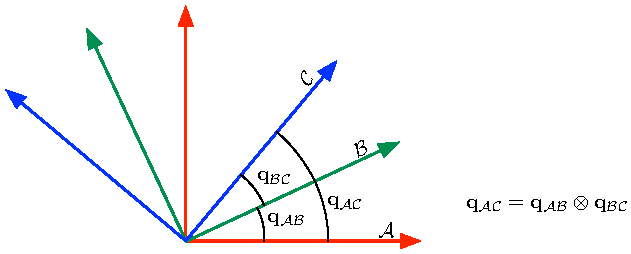
\includegraphics{figures/composition}
\caption{旋转组合。在 $\bbR^2$ 中,我们只需要做 $\theta_{\cA\cC} = \theta_{\cA\cB}+\theta_{\cB\cC}$,因为“加法”操作是可交换的。 
在 $\bbR^3$ 中组合满足 $\bfq_{\cA\cC} = \bfq_{\cA\cB}\ot\bfq_{\cB\cC}$ ,并且在矩阵形式中,$\bfR_{\cA\cC} = \bfR_{\cA\cB}\,\bfR_{\cB\cC}$。
这些算子是不可交换的,必须严格遵守顺序 --- 正确的符号有助于理解:`AB' 链与 `BC' 链创建 `AC'.}
\label{fig:composition}
\end{center}
\end{figure}
%

\paragraph{符号法评论}
一个正确的符号有助于确定组成中各因素的正确顺序,特别是对于几个旋转的组合 (参见 \figRef{fig:composition}).
例如,让 $\bfq_{ji}$ (分别是 $\bfR_{ji}$) 表示从情形 $i$ 到情形 $j$的旋转,即 $\bfx_j=\bfq_{ji}\ot\bfx_i\ot\bfq_{ji}^*$ (分别是 $\bfx_j=\bfR_{ji}\bfx_i$)。
然后,给定由四元数 $\bfq_{OA},\bfq_{AB},\bfq_{BC},\bfq_{OX},\bfq_{XZ}$表示的多个旋转,我们只需链接索引并得到:
%
\begin{align*}
\bfq_{OC} &= \bfq_{OA}\ot\bfq_{AB}\ot\bfq_{BC}
&
\bfR_{OC} &= \bfR_{OA}\,\bfR_{AB}\,\bfR_{BC}
~,
\end{align*}
%
并且已知相反的旋转对应于共轭, $\bfq_{ji}=\bfq_{ij}^*$,或转置,$\bfR_{ji}=\bfR_{ij}\tr$,我们也有
%
\begin{align*}
\bfq_{ZA} &= \bfq_{XZ}^*\ot\bfq_{OX}^*\ot\bfq_{OA} 
&
\bfR_{ZA} &= \bfR_{XZ}\tr\,\bfR_{OX}\tr\,\bfR_{OA} 
\\
&= \bfq_{ZX}\ot\bfq_{XO}\ot\bfq_{OA}
&
&= \bfR_{ZX}\,\bfR_{XO}\,\bfR_{OA}
~.
\end{align*}




\subsection{球面线性插值 (SLERP)}
\label{sec:slerp}

四元数对于计算正确的方向插值非常方便。 
给定由两个四元数 $\bfq_0$ 和 $\bfq_1$表示的两个方向,我们要找到一个四元数函数 $\bfq(t),~ t\in[0,1]$, 计算从 $\bfq(0)=\bfq_0$ 到 $\bfq(1)=\bfq_1$ 的线性插值。
这种插值是这样的,当 $t$ 从 $0$ 到 $1$ 演变时,物体将沿着方向 $\bfq_0$ 连续地沿固定轴以恒定速度旋转到方向 $\bfq_1$ 。

\paragraph{方法 1}
第一种方法使用四元数代数,并在 $\bbR^3$ 中遵循几何推理,这应该很容易与目前已知的资料相关连。
首先,像这样 $\bfq_1=\bfq_0\ot\Delta\bfq$ 计算从 $\bfq_0$ 到 $\bfq_1$ 的方向增量 $\Delta\bfq$ ,
%
\begin{align}
\Delta\bfq = \bfq_0^*\ot\bfq_1
~.
\end{align}
%
然后,获得相关的旋转向量, $\Delta\bfphi=\bfu\Delta\phi$ ,
%Then take a linear fraction of the involved rotation, 
通过使用对数映射,\footnote{我们可以在这里使用 $\log()$ 映射和 $\exp()$ 映射,也可以使用它们的大写形式的 $\Log()$ 映射和 $\Exp()$映射。最终得到的角度中所涉及的因子2最终是不相关的,因为它在最终公式中被抵消了。}
%
\begin{align}\label{equ:LogDq}
\bfu\,\Delta\phi = \Log(\Delta\bfq)
~.
\end{align}
%
最后,保持旋转轴 $\bfu$ 并取旋转角的线性部分, $\delta\phi=t\Delta\phi$ 。
通过指数映射,将其以四元数形式表示, $\delta\bfq=\Exp(\bfu\,\delta\phi)$,并与原四元数合成得到插值结果,
%
\begin{align}
\bfq(t) = \bfq_0\ot\Exp(t\,\bfu\,\Delta\phi)
~.
\end{align}
%
整个过程可以写成 $\bfq(t)=\bfq_0\ot \Exp(t\Log(\bfq_0^*\ot\bfq_1))$,它可以简化为
%
\begin{align}
\eqbox{
\bfq(t)=\bfq_0\ot(\bfq_0^*\ot\bfq_1)^t
}
~,
\end{align}
%
并且通常实现 (参见方程 \eqRef{equ:qa}) 为,
%
\begin{align}
\bfq(t)=\bfq_0\ot
\begin{bmatrix}
\cos (t\,\Delta\phi/2) \\ \bfu \sin (t\,\Delta\phi/2)
\end{bmatrix}
~.
\end{align}


\begin{figure}[htbp]
\begin{center}
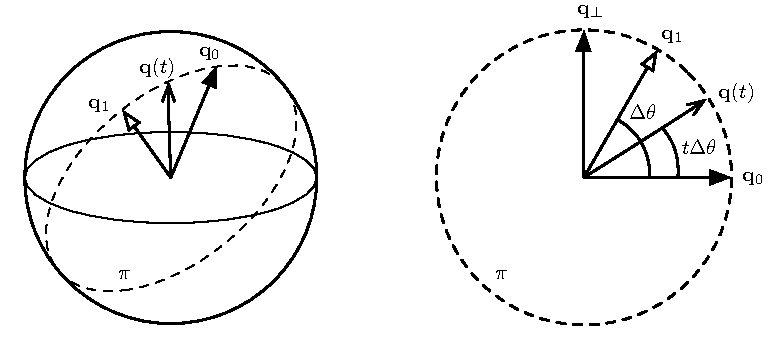
\includegraphics{figures/slerp_S4}
\caption{在 $\bbR^4$ 中的单位球中的四元数插值,以及在 $\bbR^4$ 中的旋转平面 $\pi$ 上的情况的正面视图。}
\label{fig:slerp_S4}
\end{center}
\end{figure}

\paragraph{注:} 类似的乘积可用于定义旋转矩阵的Slerp,产生
%
\begin{align}\label{equ:Rslerp}
\bfR(t)= \bfR_0\Exp(t\Log(\bfR_0\tr\bfR_1))=\bfR_0(\bfR_0\tr\bfR_1)^t 
~,
\end{align}
%
其中矩阵指数 $\bfR^t$ 可以使用 Rodrigues 公式 \eqRef{equ:rodrigues} 实现,导致
%
\begin{align}
\bfR(t)= \bfR_0 \left(\bfI + \sin(t\Delta\phi)\hatx{\bfu} + (1-\cos(t\Delta\phi))\hatx{\bfu}^2\right)
~.
\end{align}


\paragraph{方法 2}
可以开发出与四元数代数的内部无关,甚至与嵌入弧形的空间的维数无关的其它Slerp方法。 
特别是, 参见 \figRef{fig:slerp_S4},我们可以将四元数 $\bfq_0$ 和 $\bfq_1$ 视为单位球体中的两个单位向量,并在同一空间中进行插值。 
插值 $\bfq(t)$ 是单位向量,以恒定角速度
以最短球面路径从 $\bfq_0$ 到 $\bfq_1$ 进行连接。
该路径是单位球体与由 $\bfq_0$, $\bfq_1$ 和原点 (图中的虚线圆周)定义的平面相交产生的平面弧的结果。
有关这些方法与上述方法等效的证明,请参见 \cite{DAM-1998} 的论文。

这些方法的第一方法是使用向量代数,并严格遵循上述思想。 
把 $\bfq_0$ 和 $\bfq_1$ 做为两个单位向量;
%
%This angle%
它们之间的夹角%
\footnote{这个角度 $\Delta\theta=\arccos(\bfq_0\tr\bfq_1)$ 是欧几里德 4-space 中两个四元数向量之间的夹角,而不是 3D 空间中的实际旋转角度,这旋转角度从方程 \eqRef{equ:LogDq} 得到的是 $\Delta\phi=\norm{\Log(\bfq_0^*\ot\bfq_1)}$。参见 \secRef{sec:double_cover} 获得更多详细信息。}
由标量积导出,
%
\begin{align}\label{equ:slerp_angle}
\cos(\Delta\theta)&=\bfq_0\tr\bfq_1 & \Delta\theta&=\arccos(\bfq_0\tr\bfq_1)
~.
\end{align}
%
我们按以下步骤进行。 
我们识别了旋转平面,我们在这里命名为 $\pi$,
并且建立了它的正交正态基(ortho-normal basis) $\{\bfq_0,\bfq_\bot\}$,其中 $\bfq_\bot$ 来自于对 $\bfq_0$ 的正交正态化(ortho-normalizing) $\bfq_1$ ,
%
\begin{align}
\bfq_\bot &= \frac{\bfq_1-(\bfq_0\tr\bfq_1)\bfq_0}{\norm{\bfq_1-(\bfq_0\tr\bfq_1)\bfq_0}}
~,
\end{align}
%
所以 (参见 \figRef{fig:slerp_S4} --- 右边)
%
\begin{align} \label{equ:q1}
\bfq_1 = \bfq_0 \cos \Delta\theta + \bfq_\bot \sin \Delta\theta
~.
\end{align}
%
然后,我们只需要转动 $\bfq_0$ 一个角度的一部分, $t\Delta\theta$,在平面 $\pi$上,
以得到球面插值,
%
\begin{align}\label{equ:slerp_rot}
\eqbox{
\bfq(t) = \bfq_0 \cos(t\Delta\theta) + \bfq_\bot\sin(t\Delta\theta)
}
~.
\end{align}


\paragraph{方法 3}
一个类似的方法,归功于 Glenn Davis 在论文 \cite{SHOEMAKE-1985}中的观点,它从一个事实出发:连接 $\bfq_0$ 到 $\bfq_1$ 的大弧线上的任何一点都必须是其端点的线性组合 (因为这三个向量是共面的)。
利用方程 \eqRef{equ:slerp_angle} 计算出角度 $\Delta\theta$ 后,
%
%%\footnote{
%This formula can also be derived from \eqRef{equ:slerp_rot} by noticing that $\bfq_1 = \bfq_0 \cos \Delta\theta + \bfq_\bot \sin \Delta\theta$, isolating 
%
我们可以从方程 \eqRef{equ:q1} 中分离出 $\bfq_\bot$ 并且把它注入到方程 \eqRef{equ:slerp_rot} 。 应用恒等式 $\sin(\Delta\theta-t\Delta\theta)=\sin \Delta\theta\cos t\Delta\theta-\cos \Delta\theta\sin t\Delta\theta$,我们得到戴维斯公式(Davis' formula) (另一个推导参见 \cite{EBERLY-2010}论文),
%
\begin{align}
\eqbox{
\bfq(t)=\bfq_0\frac{\sin((1-t)\Delta\theta)}{\sin(\Delta\theta)}+\bfq_1\frac{\sin(t\Delta\theta)}{\sin(\Delta\theta)}
}
~.
\end{align}
%
这公式具有对称性的优点:定义反向插值器  $s=1-t$ 产生
%
\begin{align*}
\bfq(s)=
\bfq_1\frac{\sin((1-s)\Delta\theta)}{\sin(\Delta\theta)}
+
\bfq_0\frac{\sin(s\Delta\theta)}{\sin(\Delta\theta)}
~.
\end{align*}
%
这与 $\bfq_0$ 和 $\bfq_1$ 的角色互换的公式完全相同。
$\bfq_1'=-\bfq_1$$\bfq'(t)$,则沿$\bfx_0$到$\bfx_1$的最短路径产生向量$\bfx'(t)$。

\begin{figure}[htbp]
\begin{center}
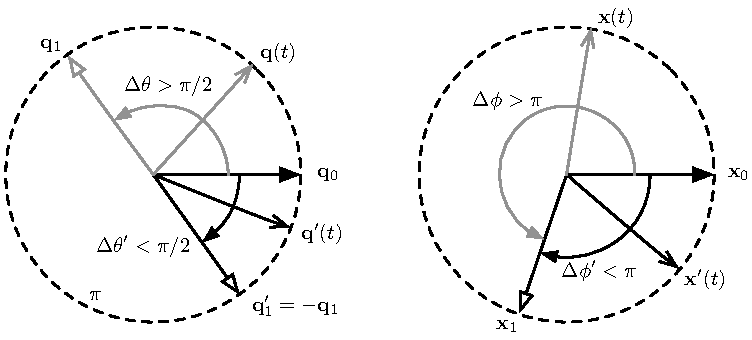
\includegraphics{figures/slerp_fix}
\caption{确保沿 $\bfq_0$ 和 $\bfq_1$表示的方向之间的最短路径进行Slerp。左边:4D 空间中的四元数旋转平面,显示初始和最终方向四元数,以及两个可能的插值,$\bfq(t)$ 从 $\bfq_0$ 到 $\bfq_1$,并且 $\bfq'(t)$ 从 $\bfq_0$ 到 $-\bfq_1$。右边:3D空间中的向量旋转平面: 
因为 $\bfq_1=-\bfq_1$,我们有 $\bfx_1=\bfq_1\ot\bfx_0\ot\bfq_1^*=\bfq_1'\ot\bfx_0\ot\bfq_1'^*$,也就是说,两个四元数产生相同的旋转。
但是,插值的四元数 $\bfq(t)$ 乘以向量 $\bfx(t)$ 将带来从 $\bfx_0$ 到 $\bfx_1$ 的长路径, 
而用 $\bfq_1'=-\bfq_1$ 修正后产生的 $\bfq'(t)$, 乘以向量 $\bfx'(t)$ ,则沿着从 $\bfx_0$ 到 $\bfx_1$ 的最短路径旋转。}
\label{fig:slerp_fix}
\end{center}
\end{figure}

所有这些基于四元数的SLERP方法都需要注意确保沿最短路径,即旋转角 $\phi\leq\pi$,进行适当的插值。
由于 $SO(3)$ 的四元数双倍覆盖(参见 \secRef{sec:double_cover}),只有锐角 $\Delta\theta\leq\pi/2$ 的四元数之间的插值是按照最短路径进行的 (\figRef{fig:slerp_fix})。
测试这种情况并解决它很简单:如果 $\cos(\Delta\theta)=\bfq_0\tr\bfq_1<0$,则将 \eg~$\bfq_1$ 替换为 $-\bfq_1$ 并重新开始。



\subsection{四元数和等倾旋转:解释魔法}
\label{sec:isoclinic}

本节提供了关于四元数的两个有趣问题的几何见解,我们称之为“魔法”:
\begin{itemize}
\item
乘积 $\bfq\ot\bfx\ot\bfq^*$ 如何旋转向量 $\bfx$ ?
\item
为什么我们在通过 $\bfq=e^{\bfphi/2}=[\cos \phi/2 , \bfu\sin\phi/2]$ 构造四元数时需要考虑半角?
\end{itemize}
%
我们需要一个几何解释,就是超出代数证明方程 \eqRef{equ:quatRotFormula} 和 \secRef{sec:double_cover} 中的双倍覆盖事实的一些基本原理。

首先,让我们在这里再现方程 \eqRef{equ:quatRotMatrixForm} ,通过在方程 \eqRef{equ:quatMatrix} 中定义的 $\QL{\bfq}$ 和 $\QR{\bfq^*}$ 的四元数乘积矩阵,来表示四元数旋转动作,
%
\begin{align*}
\bfq\otimes
\bfx\otimes\bfq^*
&= \QR{\bfq^*}\,\QL{\bfq}\begin{bmatrix}
0 \\ \bfx
\end{bmatrix} 
= \begin{bmatrix}
0 \\ \bfR\,\bfx
\end{bmatrix} 
~.
\end{align*}
%
对于单位四元数 $\bfq$,四元数乘积矩阵 $\QL{\bfq}$ 和 $\QR{\bfq^*}$ 满足两个显著性质,
%
%
\begin{align}
 \Q{\bfq}\,\Q{\bfq}\tr &= \bfI_4 \\
 \det(\Q{\bfq}) &= +1 
 ~, 
\end{align}%
%
并且是 $SO(4)$的元素,即是 $\bbR^4$ 空间中的适当旋转矩阵。 
更具体地说,它们代表了一种特殊的旋转类型,叫做等倾旋转(\emph{isoclinic rotation}),就如我们在后面解释的那样。
因此,根据方程 \eqRef{equ:quatRotMatrixForm} ,四元数旋转对应于 $\bbR^4$ 中的两个链式等倾旋转。

为了解释四元数旋转的含义, % in $\bbR^3$, 
我们需要理解 $\bbR^4$ 中的等倾旋转。
为此,我们首先需要理解 $\bbR^4$ 中的一般旋转。
并且为了理解 $\bbR^4$中的旋转,我们需要回到 $\bbR^3$ ,其旋转实际上是平面旋转。
让我们一步一步地来讨论这个问题。


\paragraph{在 $\bbR^3$ 中的旋转:} 
%
在 $\bbR^3$ 中,让我们考虑向量 $\bfx$ 围绕表示的任意轴的向量 $\bfu$的旋转 --- 参见 \figRef{fig:isoclinic3},并回忆 \figRef{fig:rotation3d}。
在旋转时,与旋转轴 $\bfu$ 平行的向量不移动,而垂直于轴的向量在垂直于轴线的平面 $\pi$ 中旋转。 
对于一般向量 $\bfx$,向量在平面内的两个分量在这个平面内旋转,而轴向分量保持静止。
%
\begin{figure}[tb]
\begin{center}
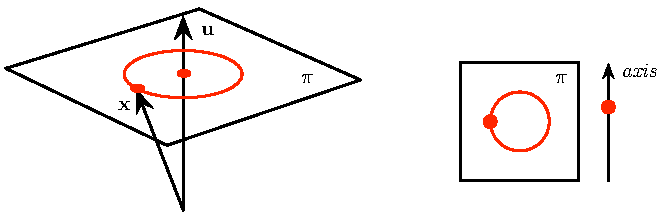
\includegraphics{figures/isoclinic3}
\caption{%
在 $\bbR^3$ 中的旋转。 
向量 $\bfx$ 围绕旋转轴 $\bfu$ 的旋转描述了一个与轴垂直的平面上的圆周。 
与轴 $\bfx$ 平行的量不移动,并且由轴上的小红点表示。
右边的草图说明了平面和轴子空间上旋转点的根本不同的行为。 
}
\label{fig:isoclinic3}
\end{center}
\end{figure}


\paragraph{在 $\bbR^4$ 中的旋转} 
%
在 $\bbR^4$ 中,参见 \figRef{fig:isoclinic4},由于额外的维度,在 $\bbR^3$ 中的一维旋转轴变为新的二维平面。
%
\begin{figure}[tb]
\begin{center}
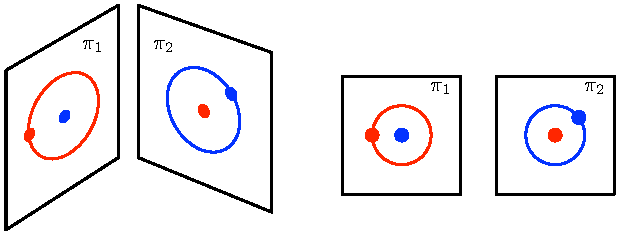
\includegraphics{figures/isoclinic4}
\caption{%
在 $\bbR^4$ 中的旋转。 
两个正交旋转是可能的,在两个正交平面 $\pi_1$ 和 $\pi_2$ 上面。 
在 $\pi_1$ 平面上旋转向量 $\bfx$ (未绘制) 导致向量的平行于该平面的两个分量 ($\pi_1$ 上的红点) 描绘了一个圆周 (红圈),
剩下在 $\pi_2$ 中的两部分不变 (红点)。
相反,在 $\pi_2$ 平面上的旋转(在 $\pi_2$ 中蓝色圆上的蓝点),剩下在 $\pi_1$ 中的两部分不变 (蓝点)。
右边的草图更好地说明了这一情况,它放弃在 $\bbR^4$中绘制不可显示的透视图,这可能会产生误导。
}
\label{fig:isoclinic4}
\end{center}
\end{figure}
%
第二个平面为第二个旋转提供了空间。
实际上,在 $\bbR^4$ 中的旋转包含在 4-space 中的两个正交平面上的两个独立的旋转。 
这意味着每个平面的每个 4-vector 在其自身的平面中旋转,并且一般 4-vectors 相对于一个平面的旋转不影响另一个平面中的向量分量。 
因为这个原因,这些平面被称为“不变量”(\emph{`invariant'})。

\paragraph{在 $\bbR^4$ 中的等倾旋转:} 
%
等倾旋转 (Isoclinic,来自希腊语,\emph{iso:} ``equal'', \emph{klinein:} ``to incline'') 是指在 $\bbR^4$ 中的旋转,在两个不变的平面中的旋转角度具有相同的大小。
然后,当两个角也有相同的符号时,%
\footnote{给定这两个不变平面,我们任意选择它们的方向,这样我们就可以在它们中关联正旋转角度和负旋转角度。}
我们说的是左等倾旋转(\emph{left-isoclinic rotations})。 
并且当它们有相反的符号时,我们说的是右等倾旋转(\emph{right-isoclinic rotations})。
%
等倾旋转的一个显著性质,我们已经在方程 \eqRef{equ:PQ_commute} 中看到过,就是左倾旋转和右等倾旋转相互交换,
\begin{align}
 \QR{\bfp}\,\QL{\bfq} = \QL{\bfq}\,\QR{\bfp}~. \label{equ:isoclinic_commute}
\end{align}

\paragraph{四元数在 $\bbR^4$ 和 $\bbR^3$ 中的旋转:}
% 
给定单位四元数 $\bfq=e^{\bfu\,\theta/2}$, 表示在 $\bbR^3$ 中围绕着旋转轴 $\bfu$ 转过一个角度 $\theta$ 的一个旋转,
矩阵 $\QL{\bfq}$ 是在 $\bbR^4$ 中的左倾旋转,对应于四元数 $\bfq$的左乘,
而  $\QR{\bfq^*}$ 是右等倾旋转,对应于四元数 $\bfq^*$的右乘。 
这些等倾旋转的角度大小正好是 $\theta/2$,%
\footnote{这可以通过提取等倾旋转矩阵的特征值来检查:它们由相位等于 $\pm\theta/2$的共轭复数对构成。}
并且不变平面是相同的。
然后,旋转表达方程 \eqRef{equ:quatRotMatrixForm} 在这里再次再现,
%
\begin{align*}
\begin{bmatrix}
0 \\ \bfx'
\end{bmatrix}=\bfq\otimes\bfx\otimes\bfq^*
&= \QR{\bfq^*}\,\QL{\bfq}\begin{bmatrix}
0 \\ \bfx
\end{bmatrix} 
~,
\end{align*}
%
表示到 4-vector $(0,\bfx)\tr$ 的两个链式等倾旋转,一个是左旋转,一个是右旋转,每个是 $\bbR^3$ 中所需旋转角度的一半。 
在 $\bbR^4$ 中的一个不变平面(参见 \figRef{fig:isoclinicQ})中,这两个半角会抵消,因为它们有相反的符号。 
%
\begin{figure}[tb]
\begin{center}
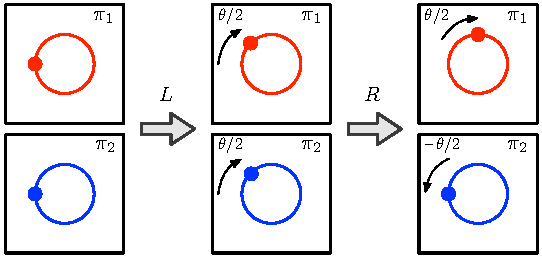
\includegraphics{figures/isoclinicQ}
\caption{%
在 $\bbR^4$ 中的四元数旋转。
两个链式等倾旋转,一个左 (具有相等的半角),一个右 (具有相反的半角),仅在一个不变平面上产生全角度的纯旋转。
}
\label{fig:isoclinicQ}
\end{center}
\end{figure}
%
在另一个平面上,它们相加得到总旋转角 $\theta$ 。 
如果我们从方程 \eqRef{equ:quatRotMatrixForm} 定义旋转矩阵, $\bfR_4$, 的结果,人们很容易意识到这点 (另见方程 \eqRef{equ:isoclinic_commute} ),
%
\begin{align}\label{equ:R4}
\bfR_4 \triangleq \QR{\bfq^*}\QL{\bfq}=\QL{\bfq}\QR{\bfq^*}= \begin{bmatrix}
1 & \bf0 \\
\bf0 & \bfR
\end{bmatrix}
~,
\end{align}
%
其中 $\bfR$ 是 $\bbR^3$中的旋转矩阵,它清晰地旋转 $\bbR^4$ 的子空间 $\bbR^3$ 中的向量,保持第四维不变。



这一论述有些超出了本文件的范围。 
它也是不完整的,因为除了方程 \eqRef{equ:R4} 中的结果之外,它并没有提供一个直观的或几何的解释,解释为什么我们需要做 $\bfq\ot\bfx\ot\bfq^*$ 而不是 \eg~$\bfq\ot\bfx\ot\bfq$ 。\footnote{就这么说吧, $\bfq\ot\bfx\ot\bfq^*$ 为旋转工作,如果 $\bfq$ 是单位四元数。实际上在 $\bbR^3$ 中如果 $\qv$ 是一个单位纯(\emph{pure})四元数,乘积 $\qv\ot\bfx\ot\qv$ 产生反射 (而不是旋转!) 。最后,乘积 $\bfq\ot\bfx\ot\bfq$,用 $\bfq$ ,一个单位非纯(\emph{non-pure})四元数,没有显著的特性。}
我们把它放在这里只是为了提供另一种解释四元数旋转的方法,希望读者能对它的机制有更多的直觉。
建议感兴趣的读者查阅有关 $\bbR^4$ 中等倾旋转的适当文献。






%=============================================================
\section{四元数约定。我的选择。}
\label{sec:conventions}

\subsection{四元数风味}

有几种方法可以确定四元数。它们基本上与四种二进制选择相关:
%
\begin{itemize}
\item
元素的顺序 --- 实数部分是第一个或最后一个:
\begin{align}
\bfq = \begin{bmatrix}
q_w \\ \qv
\end{bmatrix} 
\qquad \textit{vs.} \qquad 
\bfq = \begin{bmatrix}
\qv \\ q_w
\end{bmatrix}~.
\label{equ:quatOrder}
\end{align}

\item
乘法公式 --- 四元数代数的定义:
%
\begin{subequations}
\label{equ:quatAlg}
\begin{align}
ij=-ji=k 
\qquad \textit{vs.} \qquad 
ji=-ij=k~,
\label{equ:quatAlgDef}
\end{align}
%
分别对应不同的惯用手:
%
\begin{align}
\textit{右手(right-handed)
\qquad vs. \qquad
左手(left-handed)}~.
\label{equ:quatHand}
\end{align}
\end{subequations}
%
这意味着,给定一个旋转轴 $\bfu$,一个四元数 $\bfq_{right}\{\bfu\,\theta\}$ 使用右手规则,围绕 $\bfu$ 旋转向量一个角度 $\theta$ ,而另一个四元数 $\bfq_{left}\{\bfu\,\theta\}$ 使用左手规则。

\item
旋转算子的功能 --- 旋转坐标系或旋转向量:
%
\begin{align}
\textit{被动(Passive)
\qquad vs. \qquad
主动(Active)。}
\label{equ:quatAlibi}
\end{align}

\item
在被动情况下,操作方向 --- 局部到全局(local-to-global)或全局到局部(global-to-local):
%
\begin{align}
\bfx_{global} = \bfq\otimes\bfx_{local}\otimes\bfq^*
\qquad vs. \qquad 
\bfx_{local} = \bfq\otimes\bfx_{global}\otimes\bfq^*
\label{equ:quatInterpret}
\end{align}


\end{itemize}

这种多样的选择导致12种不同的组合。历史的发展使一些约定优于其它约定~\citep{CHOU-92,yazell-09}。
今天,在现有的文献中,我们发现了许多四元数的口味,如 
the Hamilton, 
the STS\footnote{Space Transportation System, commonly known as NASA's Space Shuttle.}, 
the JPL\footnote{Jet Propulsion Laboratory.}, 
the ISS\footnote{International Space Station.}, 
the ESA\footnote{European Space Agency.}, 
the Engineering, 
the Robotics, 
可能还有更多的宗派。 
其中许多形式可能是相同的,其它的则不是,但很少明确说明这一事实, 
很多工作对四元数关于上述四种选择的描述都不够充分。

这些差异以不明显的方式影响各自的旋转、组合等公式。 
因此,这些公式是不相容的,我们需要从一开始就作出明确的选择。

最常用的两个约定,也有最好的文档化,是 Hamilton (在方程 \eqsRef{equ:quatOrder}{equ:quatInterpret} 中左边的选项) 和 JPL (右边的选项,除了方程 \eqRef{equ:quatAlibi} 之外)。
 \tabRef{tab:Hamilton_vs_JPL} 显示了它们的特征概要。 
JPL 主要用于航空航天领域,而 Hamilton 在机器人等其它工程领域更为常见 --- 尽管这不应被视为一条规则。


\begin{table*}
\renewcommand{\arraystretch}{1.3}
\centering
\caption{Hamilton vs. JPL quaternion conventions \wrt the 4 binary choices}
\vspace{1ex}
\begin{tabular}{|cl|c|c|}
\hline
& Quaternion type & Hamilton & JPL \\
\hline\hline
1 & Components order & $(q_w \,,\, \qv)$ & $(\qv \,,\, q_w)$ \\
\hline
\multirow{2}{*}{2} & Algebra & $ij=k$ & $ij=-k$ \\
& Handedness & Right-handed & Left-handed \\
\hline
3 & Function & Passive & Passive
\\
\hline
\multirow{3}{*}{4} & Right-to-left products mean & Local-to-Global & Global-to-Local \\
& Default notation, $\bfq$ & $\bfq \triangleq \bfq_{\cG\cL}$ & $\bfq \triangleq \bfq_{\cL\cG}$ \\
& Default operation & $\bfx_\cG = \bfq\otimes\bfx_\cL\otimes\bfq^*$ & $\bfx_\cL = \bfq\otimes\bfx_\cG\otimes\bfq^*$ \\
\hline
\end{tabular}
\label{tab:Hamilton_vs_JPL}
\end{table*}

我的选择,早在方程 \eqRef{equ:quatAlgebra} 中就已经被采纳,是采用 Hamilton 约定, 
它是右手规则,在机器人学中广泛使用的许多软件库,如 Eigen, ROS, Google Ceres, 
以及大量关于利用IMUs进行姿态估计的 Kalman 滤波的文献中广泛使用~\citep[还有更多其它的例子]{CHOU-92,KUIPERS-99,PINIES-07,ROUSSILLON-11a,MARTINELLI-12}。

而 JPL 约定可能不太常用,至少在机器人领域是这样。 
这在~\citep{TRAWNY-05-QUAT}中有广泛的描述,这是一个目标和范围非常接近于当前的参考著作,但仅集中在 JPL 约定。 
JPL 四元数被使用在 JPL 文献中 (显然的) 并在 Li, Mourikis, Roumeliotis, 和其同事撰写的关键论文中使用 (参见 \eg~\citep{LI-2012,LI-14}),这描述来自 \citeauthor{TRAWNY-05-QUAT}' 的文件。 
这些工作是处理视觉惯性测距和 SLAM 时的灵感的根本来源 --- 这就是我们所做的。 

在本节的其余部分中,我们将更深入地分析这两个四元数约定。


%-------------------------------------------------------------
\subsubsection{四元数组分的顺序}

虽然不是最基本的,但 Hamilton 和 JPL 四元数之间最显著的区别在于组分的顺序,标量部分要么在第一位置 (Hamilton) ,要么在最后位置 (JPL) 。 
这种变化的影响是相当明显的,不应代表对解释的巨大挑战。 
事实上,一些四元数实数组分在最后的软件 (\eg, the C++ library Eigen) 仍然被认为是使用 Hamilton 约定,只要其它三个方面得以维持。

我们使用下标 $(w, x, y, z)$ 表示四元数组分,以提高清晰度,而不是其它常用的 $(0, 1, 2, 3)$ 。
当改变顺序时, $q_w$ 总是表示实部,而 $q_0$ 是否也会这样做还不清楚 
--- 某些情况下,人们可能会发现一些问题,比如 $\bfq=(q_1, q_2, q_3, q_0)$ ,用 $q_0$ 表示实数并放在最后,但是在一般情况下 $\bfq=(q_0, q_1, q_2, q_3)$,最后的实部是 $q_3$。%
\footnote{另见脚注 \ref{ftn:quatComponents}。} 
当从一个约定变化到另一个约定时,我们必须小心公式中涉及全部 $4\times4$ 或 $3\times4$ 四元数相关矩阵, 
因为它们的行和/或列需要交换。 
这不难做到,但可能很难检测,因此容易出错。

关于组分顺序的两个奇怪之处是:
%
\begin{itemize}
\item
先有实数部分,四元数自然被解释为一个扩展复数,这是是熟悉的形式 \emph{real+imaginary}。
我们中的一些人对此表示满意,可能是因为这个原因。
\item
实数部分在最后,四元数以向量形式表示,
%
$\bfq=\begin{bmatrix}
x,y,z,w
\end{bmatrix}\in\bbH$, 
%
其格式与射影 3D 空间中的齐次向量完全等价, 
%
$\bfp=\begin{bmatrix}
x,y,z,w
\end{bmatrix}\in\bbP^3$, 
%
在这两种情况下 $x,y,z$ 都与三个笛卡尔轴有明确地标识。 
在处理 3D 几何问题时,这使得四元数和齐次向量上的运算代数更加一致, 
特别是 (但不仅如此) 如果齐次向量被约束到单位球面 $\norm{\bfp}=1$ 上。
\end{itemize}

%-------------------------------------------------------------
\subsubsection{四元数代数的规范}


Hamilton 约定定义了 $ij=k$ 并因此,
%
\begin{align}
i^2 = j^2 = k^2 = ijk = -1~,\quad ij = -ji = k~, \quad jk = -kj = i~, \quad ki = -ik = j~,
\end{align}
%
而 JPL 约定定义 $ji=k$ 并因此其四元数代数变成为,
%
\begin{align}
i^2 = j^2 = k^2 = -ijk = -1~,\quad -ij = ji = k~, \quad -jk = kj = i~, \quad -ki = ik = j~.
\end{align}

有趣的是,这些细微的符号变化保留了四元数作为旋转算子的基本性质。 
数学上,关键的结果是方程 \eqRef{equ:quatProdVec} 中叉积符号的变化,这导致四元数惯用手的变化~\citep{SHUSTER-93}:
Hamilton 使用 $ij=k$ 并因此是右手的,即,它按照右手规则旋转向量; JPL 使用 $ji=k$ 并因此是左手的~\citep{TRAWNY-05-QUAT}. 
作为相反符号的左手和右手旋转,我们可以说它们的四元数 $\bfq_{left}$ 和 $\bfq_{right}$ 相关于,
%
\begin{align}
\bfq_{\textit{left}}= \bfq_{\textit{right}}^*~.
\end{align}



%-------------------------------------------------------------
\subsubsection{旋转算子的功能}

我们已经看到了如何在3D中旋转向量。这在~\citep{SHUSTER-93} 中被称为主动(\emph{active})解释, 
因为算子 (这影响所有的旋转算子) 主动旋转向量,
%
\begin{align}
\bfx' &=\bfq_{\textit{active}}\otimes\bfx\otimes\bfq_{\textit{active}}^* ~,
& 
\bfx' &= \bfR_{\textit{active}}\,\bfx~.
\end{align}

观察向量 $\bfx$ 上 $\bfq$ 和 $\bfR$ 的效果的另一种方法是,考虑向量是稳定的,但我们已经将我们的视角旋转了 $\bfq$ 或 $\bfR$ 指定的量。 
这被称为坐标系变换(\emph{frame transformation}),并且它在~\citep{SHUSTER-93}中称为被动(\emph{passive})解释,因为向量不移动,
%
\begin{align}
\bfx_\cB &= \bfq_{\textit{passive}}\ot\bfx_\cA\ot\bfq_{\textit{passive}}^*~,
&
\bfx_\cB&=\bfR_{\textit{passive}}\,\bfx_\cA~,
\end{align}
%
其中 $\cA$ 和 $\cB$ 是两个笛卡尔坐标系,并且 $\bfx_\cA$ 和 $\bfx_\cB$ 是这些坐标系中相同向量 $\bfx$ 的表达式。 
有关解释和正确的符号,请参阅下面的内容。


主动解释和被动解释由相互相反的算子控制,即, 
%
\begin{align*}
\bfq_{\textit{active}} &= \bfq_{\textit{passive}}^* ~,
& 
\bfR_{active} &= \bfR_{passive}\tr ~.
\end{align*}
%
Hamilton 和 JPL 都使用被动约定。 

\paragraph{方向余弦矩阵}
有一些作者认为被动算子不是旋转算子,而是一个方向规范,叫做方向余弦矩阵(\emph{direction cosine matrix}),
%
\begin{align}
\bfC = \begin{bmatrix}
c_{xx} & c_{xy} & c_{zx} \\
c_{xy} & c_{yy} & c_{zy} \\
c_{xz} & c_{yz} & c_{zz} 
\end{bmatrix}
~,
\end{align}
%
其中每个组分 $c_{ij}$ 都是源坐标系中的 $i$ 轴与目标坐标系中的 $j$ 轴之间的夹角余弦。我们有特征值,
%
\begin{align}
\bfC \equiv \bfR_{\textit{passive}}
~.
\end{align}


%-------------------------------------------------------------
\subsubsection{旋转算子的方向}

在被动情况下,第二解释源与旋转矩阵和四元数的操作方向相关, 
可以从局部坐标系转换为全局坐标系,也可以从全局坐标系转换为局部坐标系。 

给定两个笛卡尔坐标系 $\cG$ 和 $\cL$,我们将 $\cG$ 和 $\cL$ 标识为全局和局部坐标系。
``全局(Global)'' 和 ``局部(local)'' 是相对定义,即 $\cG$ 是全局的,相对于 $\cL$,并且 $\cL$ 是局部的,相对于 $\cG$ --- 换句话说, $\cL$ 是在参考坐标系 $\cG$中指定的坐标系。\footnote{其它通用的 \{global, local\} 坐标系是 \{parent, child\} 和 \{world, body\}。第一种方法在一个系统中涉及两个以上的坐标系时比较方便 (例如,仿人机器人中每个运动环节的坐标系);第二种方法对一个被标识为世界的唯一参考坐标系中的实体 (例如,飞机、汽车) 的移动比较方便。} 
我们指定 $\bfq_{\cG\cL}$ 和 $\bfR_{\cG\cL}$ 分别是从坐标系 $\cL$ 到坐标系 $\cG$ 的四元数和旋转矩阵转换向量, 
从某种意义上说,向量 $\bfx_\cL$ 在坐标系 $\cL$ 中被坐标系 $\cG$ 用四元数和矩阵乘积表示,
%
\begin{align}
\bfx_\cG &= \bfq_{\cG\cL}\otimes\bfx_\cL\otimes\bfq_{\cG\cL}^*~, &
\bfx_\cG &= \bfR_{\cG\cL}\,\bfx_\cL~.
\label{equ:local_to_global}
\end{align}
%
相反的转换,从 $\cG$ 到 $\cL$,是用
%
\begin{align}
\bfx_\cL &= \bfq_{\cL\cG}\otimes\bfx_\cG\otimes\bfq_{\cL\cG}^*
~,
&
\bfx_\cL &= \bfR_{\cL\cG}\,\bfx_\cG~,
\end{align}
%
其中
%
\begin{align}
\bfq_{\cL\cG} &= \bfq_{\cG\cL}^*~,
& 
\bfR_{\cL\cG} &= \bfR_{\cG\cL}\tr~. \label{equ:localVsGlobal}
\end{align}


Hamilton 使用局部到全局(local-to-global)作为以坐标系 $\cG$ 表示的坐标系 $\cL$ 的默认规范, 
%
\begin{align}
\bfq_{\textit{Hamilton}} \triangleq \bfq_{[\textit{with~respect~to}][\textit{of\,}]}=\bfq_{[\textit{to}][\textit{from}]}=\bfq_{\cG\cL}~, 
\end{align}
%
而 JPL 使用相反的全局到局部(global-to-local)转换,
%
\begin{align}
\bfq_{\textit{JPL}} \triangleq \bfq_{[\textit{of}\,][\textit{with~respect~to}]}=\bfq_{[\textit{to}][\textit{from}]}=\bfq_{\cL\cG}~.
\end{align}

请注意
%
\begin{align}
\bfq_{\textit{JPL}}
\triangleq    \bfq_{\cL\cG,left}
=    \bfq_{\cL\cG,\textit{right}}^*
=    \bfq_{\cG\cL,\textit{right}}
\triangleq    \bfq_{\textit{Hamilton}}%^*
~,
\label{equ:quatEquivalences}
\end{align}
%
这并不特别有用,但它说明了在混合约定时容易混淆。
还要注意,我们可以得出结论, $\bfq_{JPL} = \bfq_{Hamilton}$,但这远远不是一个漂亮的结果,只是一个非常混乱的来源, 
因为等式只存在于四元数值中, 
但是这两种四元数在公式中使用时,意味着和代表着不同的东西。




%%-------------------------------------------------------------
%\subsection{Notation}
%
%An often underestimated source of confusion when dealing with quaternion algebra is related to notation. 
%We believe notation should be clear, lightweight and unambiguous. 
%Of course, this applies not only to quaternions and rotation matrices, but also to the points and vectors manipulated by these. 
%A good notation requires considering many conflicting aspects: 
%%
%\begin{itemize}
%
%\item 
%Clearly distinguish scalars, vectors, matrices and functions with different font styles.
%
%\item
%Use the main letter to signify the physical dimension. Use prefixes, subscripts, superscripts and/or accents for details and particularities.
%
%\item Avoid tiny elements such as tildes $\tilde\bfq$, hats $\hat\bfq$, bars $\bar\bfq$, $\ul\bfq$, and other accents, as much as possible.
%
%%\item Avoid making extensive use of unusual Greek symbols. 
%%If we cannot tell a symbol name, then we cannot read a formula. What is $\Xi$? And $\Upsilon$?
%
%\item Avoid certain combinations of subscripts and superscripts on the left and right hand sides, %\eg, $^ix_j$, 
%especially when they appear in multiple levels, \eg, $^{C_i}x_{F_j}$. 
%They produce formulas such as $^iu_j=\frac{^{C_i}x_{F_j}}{^{C_i}z_{F_j}}$ (which is the pinhole camera model) that are difficult to read because the main variables, $x$ and $z$, are not salient enough.
%
%\item Make composition of chains obviously and unambiguously readable. 
%For example, the rotation matrix $\bfR_\cA^\cB$ or the quaternion $ _\cA^\cB\bfq$ are ambiguous because we do not know if they transform ``$\cA$ to $\cB$\,'' or ``$\cB$ to $\cA$''.
%
%
%\item
%Provide easy 1:1 translation to readable programming code. This last point becomes increasingly important as most of the works we produce are meant to be translated into algorithms.
%
%
%\end{itemize}
%
%Our notation derives from the following rules,
%%
%\begin{enumerate}
%\item
%Scalars are $a,x,\omega$; vectors are $\bfa,\bfx,{\bm \omega}$, matrices are $\bfA, \bfX, {\bf\Omega}$; functions are $f(), g()$. 
%
%\item
%We use decorations to provide details of a given magnitude. As an example, we use~$\bfa$ for \emph{acceleration}, and $\delta\bfa,~ \bfa_m,~ \bfa_b,~ \hat\bfa,~ \bfA,~ \bfa_n,~ \bfA_n$ respectively for \emph{acceleration error, measured acceleration, accelerometer bias, mean of the acceleration estimate, covariance of the acceleration estimate, acceleration noise, covariance of the acceleration noise}. 
%
%\item
%The only accent we use is the hat, $\hat\bfx$, to signify the mean of the Kalman filter Gaussian estimate. Error-state values are noted $\delta\bfx$. 
%
%\item
%The general translation specification $\bft$ needs 3 decorations: a translation \emph{from} point $\cB$ / \emph{to} point $\cC$ / \emph{expressed in} frame $\cA$,
%%
%\begin{align}
%\bft_{[expressed~in],[initial~point][end~point]}~.
%\end{align}
%%
%This produces forms such as $\bft_{\cA,\cB\cC}$.  
%We define two convenient simplifications:
%%
%\begin{itemize}
%\item
%When $\bft_{\cA,\cB\cC}$ refers to a point $\cP$, we consider its origin at the origin of the reference frame, \ie, $\cB=\cA$, giving 
%%
%\begin{align}
%\bfp_\cA\triangleq\bft_{\cA,\cA \cP}~. \label{equ:point}
%\end{align}
%%
%\item
%When $\bft_{\cA,\cB\cC}$ refers to a free vector $\bfv=\ol{\cB\cC}$, we may simply write 
%%
%\begin{align}
%\bfv_\cA\triangleq\bft_{\cA,\ol{\cB\cC}}~. \label{equ:vector}
%\end{align}
%%
%\end{itemize}
%%
%In both cases we keep the reference frame $\cA$ where the point or vector is expressed in. In case of no ambiguity, when this frame is the world frame $\cW$ of our application we allow us to drop this decoration too. For example, the position $\cP$ of the robot in the world frame may be denoted simply by $\bfp$,
%%
%\begin{align}
%\bfp \triangleq \bfp_\cW = \bft_{\cW,\cW \cP}~.  \label{equ:worldPoint}
%\end{align}
%
%
%\item
%The general orientation specification, $\bfq$ or $\bfR$, requires 2 decorations: a transformation \emph{from} frame $\cB$ / \emph{to} frame $\cA$, or equivalently, the orientation \emph{of} frame $\cB$ / \emph{\wrt} frame $\cA$,
%%
%\begin{align}
%\bfq_{[to][from]} &\equiv \bfq_{[with~respect~to][of]}
%~,
%&
%\bfR_{[to][from]} &\equiv \bfR_{[with~respect~to][of]}~.
%\end{align}
%%
%This produces forms such as $\bfR_{\cA\cB}$ that lead unambiguously to $\bfx_\cA=\bfR_{\cA\cB}\bfx_\cB$. 
%Stacked or composed transforms produce  chains such as 
%%
%\begin{align}
%\bfx_\cA &= \bfq_{\cA\cB}\otimes\bfq_{\cB\cC}\otimes\bfx_\cC\otimes\bfq_{\cB\cC}^*\otimes\bfq_{\cA\cB}^*~,
%& 
%\bfx_\cA &= \bfR_{\cA\cB}\,\bfR_{\cB\cC}\,\bfx_\cC 
%~. \label{equ:2frames}
%\end{align}
%%
%which are readable and not prone to error. 
%Notice how each of the two frame identifiers is always at the side of the entity nearby, creating a \emph{chain}  of identifiers.
%% (though in the quaternion transform above, this only applies to the quaternions chain on the left of the vector, the ones that are not conjugated). 
%In the quaternion case, the chain of identifiers can be made more salient by recalling that $\bfq_{\cA\cB}^*=\bfq_{\cB\cA}$ and thus 
%%
%\begin{align}
%\bfx_\cA = \bfq_{\cA\cB}\otimes\bfq_{\cB\cC}\otimes\bfx_\cC\otimes\bfq_{\cC\cB}\otimes\bfq_{\cB\cA}~.
%\end{align} 
%%
%This allows us to easily construct and/or identify frame composition chains with absolutely no ambiguity. 
%
%Oftentimes, the world frame $\cW$ and the frame of the main moving body $\cB$ may be omitted (in cases where there is no ambiguity), yielding
%%
%\begin{align}
%\bfq &\triangleq \bfq_{\cW \cB}~,
%&
%\bfR &\triangleq \bfR_{\cW \cB}~. \label{equ:rotSimp}
%\end{align}
%% 
%This, and the simplifications for points and vectors \eqsRef{equ:point}{equ:worldPoint} above, lead to 
%%
%\begin{align}
%\bfx &= \bfq\otimes\bfx_\cB\otimes\bfq^* ~, 
%&
%\bfx &= \bfR\,\bfx_\cB ~,
%\end{align}
%%
%which are very light and easy to read.
%They express the transformation of vector $X$ from the body frame $\cB$ to the world frame $\cW$.
%
%\item We use only right-hand subscripts for frame decorations. This way, translating formulas into code and vice-versa becomes straightforward. In the code, the first letter before the first underscore is always the physical magnitude. For example, these formula and code are equivalent,
%%
%\begin{align}
%\bfx_\cA &= \bfR_{\cA\cB}\,\bfR_{\cB\cC}\,\bfx_\cC~,
%& 
%\texttt{ x\_A = R\_A\_B * R\_B\_C * x\_C}~.
%\end{align}
%
%
%
%\end{enumerate}
%




%=============================================================
\section{扰动、导数和积分}


%\section{Definition of the derivatives }

\subsection{在 $SO(3)$ 中的加法和减法算子}

\begin{figure}[tb]
\centering
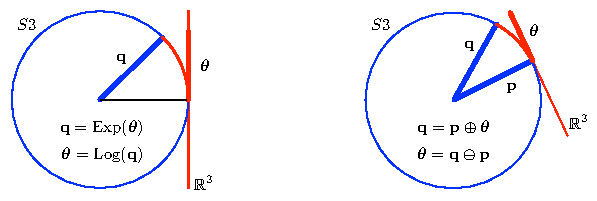
\includegraphics{figures/manifold}
\caption{在 $\bbR^4$ 中,$S3$流形是一个单位球体,这里用一个单位圆(蓝色)表示,所有单位四元数都在其中。
流形的切空间是超平面 $\bbR^3$,这里用一条线(红色)表示。
左(\emph{Left}):$\Exp()$ 和 $\Log()$ 算子将 $\bbR^3$ 的元素映射到/回 $S3$的元素。
右(\emph{Right}):$\oplus$ 和 $\ominus$ 算将流形的元素与切空间中的元素相关联。(同样,这些插图说明了 $SO(3)$ 的流形。)}
\label{fig:manifold}
\end{figure}

在向量空间 $\bbR^n$中,加法和减法运算是用正规的加法 `$+$' 和减法 `$-$' 运算来执行的。
在 $SO(3)$ 中这是不可能的,但是可以定义等价算子来建立一个合适的微积分语料库。 

因此,我们定义了在 $\sR\in SO(3)$ 中的元素之间的加法和减法算子, $\oplus,\ominus$,还有 $\sR$ 处在切空间 $\bth\in\bbR^3$ 中的元素 $\bth\in\bbR^3$ ,如下所示。

\paragraph{加法算子。}
加法(`plus')算子 $\oplus:SO(3)\times\bbR^3\to SO(3)$ 生成一个在 $SO(3)$ 中的元素 $\sS$ ,其结果为一个在 $SO(3)$ 中的参考元素 $\sR$ 的组合,并有一个(通常较小)的旋转。这个旋转是由参考元素 $\sR$ 处与 $SO(3)$ 流形相切的向量空间 $\bth\in\bbR^3$ 中的向量指定的,也就是说,
%
\begin{align}
\sS = \sR\oplus \bth &\te \sR\circ\Exp(\bth) && \sR,\sS\in SO(3),~ \bth\in\bbR^3 
~.
\end{align}
%
注意,可以为 $SO(3)$的任何表示定义此算子。特别是,对于四元数和旋转矩阵,我们有,
%
\begin{align}
\bfq_\sS &= \,\bfq_\sR\oplus\bth = \bfq_\sR\ot\Exp(\bth) \\
\bfR_\sS &= \bfR_\sR\oplus \bth = \bfR_\sR\tdot\Exp(\bth) 
~.
\end{align}

\paragraph{减法算子。}
减法(`minus')算子 $\ominus:SO(3)\times SO(3)\to\bbR^3$ 是加法算子的逆运算。它返回在 $SO(3)$ 中的两个元素之间的向量角差 $\bth\in\bbR^3$ 。这个差值在与参考元素 $\sR$ 相切的向量空间中表示,
%
\begin{align}
\bth=\sS\ominus \sR
&\te \Log(\sR\inv \circ \sS)     && \sR,\sS\in SO(3),~ \bth\in\bbR^3  
~,
\end{align}
%
其中对于四元数和旋转矩阵来说读到,
%
\begin{align}
\bth &= \,\,\bfq_\sS\ominus\bfq_\sR\, = \Log(\bfq_\sR^*\ot\bfq_\sS)                      \\
\bth &= \bfR_\sS\ominus\bfR_\sR = \Log(\bfR_\sR\tr\,\bfR_\sS)
~.
\end{align}

\bigskip
在这两种情况下,请注意,即使向量差值 $\bftheta$ 通常被认为是很小的值,上述定义对于 $\bftheta$ 的任何值(直到 $SO(3)$ 流形的第一个覆盖,即对于角 $\theta<\pi$)仍然有效。

\subsection{四种可能的导数定义}



\subsubsection{从向量空间到向量空间的函数}

标量和向量情况遵循导数的经典定义:给定一个函数 $f:\bbR^m\to\bbR^n$,我们使用 $\{+,-\}$ 将导数定义为
%
\begin{align}
\dpar{f(\bfx)}{\bfx} &\te \lim_{\delta\bfx\to0}\frac{f(\bfx+\delta\bfx)-f(\bfx)}{\delta\bfx} &&\in \bbR^{n\times m} \label{equ:derivative_vector}
\end{align}
%
欧拉积分产生形式的线性表达式
%
\begin{align*}
f(\bfx+\Delta\bfx) &\approx f(\bfx) + \dpar{f(\bfx)}{\bfx}\Delta\bfx
& \in \bbR^n
\end{align*}

\subsubsection{从 $SO(3)$ 到 $SO(3)$ 的函数}

给定一个函数 $f:SO(3) \to SO(3)$ 并有 $\sR\in SO(3)$ 和一个局部的小角度变量 $\bth\in\bbR^3$,我们使用 $\{\oplus,\ominus\}$ 将导数定义为
%
\begin{align}
\dpar{f(\sR)}{\bth} 
&\te \lim_{\delta\bth\to0}\frac{f(\sR\oplus\delta\bth)\ominus f(\sR)}{\delta\bth}  && \in \bbR^{3\times 3}\\
&= \lim_{\delta\bth\to0}\frac{\Log\big(f\inv(\sR)\,f(\sR\Exp(\delta\bth))\big)}{\delta\bth} \label{equ:derivative_SO3}
\end{align}
%
欧拉积分产生形式的表达式,
%
\begin{align*}
f(\sR\oplus\Delta\bth) &\approx f(\sR)\,\oplus\,\dpar{f(\sR)}{\bth}\,\Delta\bth
 \te f(\sR)\Exp\left(\dpar{f(\sR)}{\bth}\Delta\bth\right)
 & \in SO(3)
\end{align*}




\subsubsection{从向量空间到 $SO(3)$ 的函数}

这种情况,对于函数 $f:\bbR^m\to SO(3)$,我们使用 `+' 表示向量的扰动,并使用 `$\ominus$' 表示 $SO(3)$ 的差分,
%
\begin{align}
\dpar{f(\bfx)}{\bfx} &\te \lim_{\delta\bfx\to0} \frac{ f(\bfx+\delta\bfx)\ominus f(\bfx)}{\delta\bfx} && \in \bbR^{3\times m} \label{equ:dif_RtoSO3}\\
&= \lim_{\delta\bfx\to0} \frac{\Log(f\inv(\bfx) f(\bfx+\delta\bfx))}{\delta\bfx}
\end{align}
%
欧拉积分产生形式的表达式,
%
\begin{align*}
f(\bfx+\Delta\bfx) &\approx f(\bfx)\,\oplus\,\dpar{f(\bfx)}{\bfx}\,\Delta\bfx
 \te f(\bfx)\,\Exp\left(\dpar{f(\bfx)}{\bfx}\Delta\bfx\right)
 & \in SO(3)
\end{align*}

\subsubsection{从 $SO(3)$ 到向量空间的函数}

这种情况,对于函数 $f: SO(3)\to\bbR^n$,我们使用 `$\oplus$' 表示 $SO(3)$ 的扰动,并使用 `$-$' 表示向量差分,
%
\begin{align}
\dpar{f(\sR)}{\bth} &\te \lim_{\delta\bth\to0} \frac{f(\sR\oplus\delta\bth) - f(\sR)}{\delta\bth} && \in \bbR^{n\times 3} \label{equ:jacobian_SO3_Rn}\\
&= \lim_{\delta\bth\to0} \frac{f(\sR\Exp(\delta\bth)) - f(\sR)}{\delta\bth}
\end{align}
%
欧拉积分产生形式的表达式,
%
\begin{align*}
f(\sR\oplus\delta\bth) &\approx f(\sR)+\dpar{f(\sR)}{\bth}\,\Delta\bth
 \te f(\sR)+\Exp\left(\dpar{f(\sR)}{\bth}\Delta\bth\right)
 & \in SO(3)
\end{align*}

%=============================================================

\subsection{有用,并且非常有用,旋转的 Jacobians 矩阵}

让我们考虑围绕单位轴 $\bfu$,以 $\theta$ 弧度旋转到向量 $\bfa$。让我们用三种等价的形式来表示旋转规范,即 $\bftheta=\theta\bfu$, $\bfq=\bfq\{\bftheta\}$ 和 $\bfR=\bfR\{\bftheta\}$。 
我们对相对于不同量值的旋转结果的 Jacobians 矩阵感兴趣。


%-------------------------------------------------------------
\subsubsection{相对于向量的 Jacobian 矩阵}

向量 $\bfa$ 旋转的导数相对于这个向量是平凡的,
%
\begin{align}
\eqbox{
\dpar{(\bfq\ot\bfa\ot\bfq*)}{\bfa} = \dpar{(\bfR\,\bfa)}{\bfa} = \bfR
}
~.
\end{align}
%




%-------------------------------------------------------------
\subsubsection{相对于四元数的 Jacobian 矩阵}


相反,相对于四元数 $\bfq$ 的旋转导数是很棘手的。 
为了方便起见,我们对四元数使用了轻量级符号, $\bfq=[w~\bfv] = w+\bfv$ 。
我们使用方程 \eqRef{equ:quatProdPure} , \eqRef{equ:quatCommutatorPure},并标识为 $\bfa \times (\bfb \times \bfc) = (\bfc \times \bfb) \times \bfa = (\bfa \tr \bfc)\,\bfb - (\bfa \tr \bfb)\,\bfc$,以扩展基于旋转的四元数方程 \eqRef{equ:sandwichProd} ,如下所示,
%
\begin{align} \label{equ:drot_dtheta}
\begin{split}
\bfa' &= \bfq\ot\bfa\ot\bfq* \\
&= (w+\bfv)\ot\bfa\ot(w-\bfv) \\
&= w^2\bfa + w(\bfv\ot\bfa - \bfa\ot\bfv) - \bfv\ot\bfa\ot\bfv \\
&= w^2\bfa + 2w(\bfv\tcross\bfa) - \big[(-\bfv\tr\bfa+\bfv\tcross\bfa)\ot\bfv \big]\\
&= w^2\bfa + 2w(\bfv\tcross\bfa) - \big[(-\bfv\tr\bfa)\,\bfv+(\bfv\tcross\bfa)\ot\bfv \big]\\
&= w^2\bfa + 2w(\bfv\tcross\bfa) - \big[(-\bfv\tr\bfa)\,\bfv - \cancel{(\bfv\tcross\bfa)\tr\bfv}+(\bfv\tcross\bfa)\tcross\bfv \big]\\
%&= w^2\bfa + 2w(\bfv\tcross\bfa) - \big[(-\bfv\tr\bfa)\,\bfv+(\bfv\tcross\bfa)\tcross\bfv \big]\\
%&= w^2\bfa + 2w(\bfv\tcross\bfa) - \big[(-\bfv\tr\bfa)\,\bfv - \bfv\tcross(\bfv\tcross\bfa) \big]\\
&= w^2\bfa + 2w(\bfv\tcross\bfa) - \big[(-\bfv\tr\bfa)\,\bfv + (\bfv\tr\bfv)\,\bfa - (\bfv\tr\bfa)\,\bfv \big]\\
%&= w^2\bfa + 2w(\bfv\tcross\bfa) + (\bfv\tr\bfa)\,\bfv + (\bfv\tr\bfa)\,\bfv-(\bfv\tr\bfv)\,\bfa\\
&= w^2\bfa + 2w(\bfv\tcross\bfa) + 2(\bfv\tr\bfa)\,\bfv - (\bfv\tr\bfv)\,\bfa
~.
\end{split}
\end{align}%
%
有了这个,我们可以提取导数 $\dparil{\bfa'}{w}$ 和 $\dparil{\bfa'}{\bfv}$,
%
\begin{align}
\dpar{\bfa'}{w} &= 2(w\bfa + \bfv\tcross\bfa) \\
\begin{split}
\dpar{\bfa'}{\bfv} &= -2w\hatx{\bfa} + 2(\bfv\tr\bfa\,\bfI+\bfv\,\bfa\tr) - 2\bfa\,\bfv\tr 
\\
&= 2(\bfv\tr\bfa\,\bfI+\bfv\,\bfa\tr - \bfa\,\bfv\tr - w\hatx{\bfa} )
~,
\end{split}
\end{align}%
%
产生
%
\begin{align} \label{equ:drot_dq}
\eqbox{
\dpar{(\bfq\ot\bfa\ot\bfq*)}{\bfq} = 
%\dpar{(\bfR\,\bfa)}{\bfq} = 
2\begin{bmatrix}
~w\,\bfa + \bfv\tcross\bfa ~~ \big| ~  \bfv\tr\bfa\,\bfI_3+\bfv\,\bfa\tr - \bfa\,\bfv\tr -w\hatx{\bfa}
~\end{bmatrix} \in \bbR^{3\times 4}
}~.
\end{align}



%\subsubsection{Right Jacobian of $SO(3)$}
%
%\begin{figure}[tbp]
%\begin{center}
%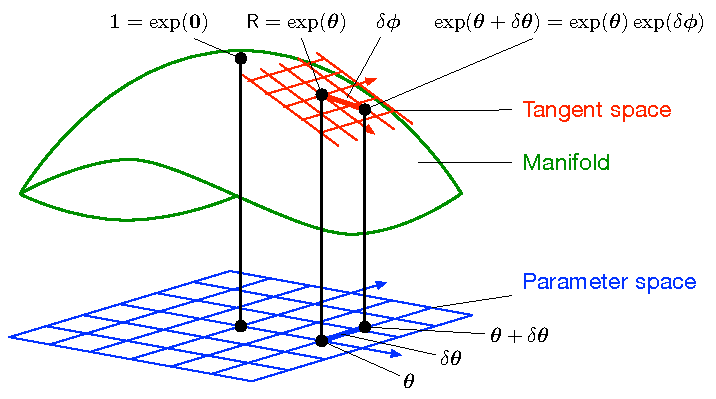
\includegraphics{figures/right_jac}
%\caption{The right Jacobian $\bfJ_r=\dparil{\delta\bfphi}{\delta\bftheta}$ maps variations $\delta\bftheta$ around the parameter $\bftheta$ into variations $\delta\bfphi$ on the vector space tangent to the manifold at the point $\Exp{\bftheta}$. }
%\label{fig:right_jac}
%\end{center}
%\end{figure}
%
%
%Let us define the `minus' operator $\ominus$ in $SO(3)$ that returns the rotation increment as a vector $\delta\bfphi$ in the tangent space $\so(3)$, that is,
%%
%\begin{align}
%\delta\bfphi = r_2 \ominus r_1 \triangleq \Log(r_1\inv\circ r_2) = \Log(\bfR_1\tr\bfR_2) = \Log(\bfq_1^*\ot\bfq_2) \in \bbR^3
%\end{align}
%%
%where $r_1,r_2$ are two elements of $SO(3)$, and $\circ$ is their composition. This `minus' operator allows us to define derivatives in $SO(3)$ in a way akin to those in Euclidean space, 
%%
%\begin{align}
%\bfJ_r(\bftheta) = \dpar{\delta\bfphi}{\delta\bftheta} 
%\triangleq 
%\lim_{\delta\bftheta\to0} \frac{r(\bftheta+\delta\bftheta)\ominus r(\bftheta)}{\delta\bftheta}
%\end{align}
%%
%%
%This derivative is a matrix, $\bfJ_r(\bftheta)\in\bbR^{3\times3}$, known as the right Jacobian of $SO(3)$.
%It maps variations around $\bftheta$ in the parameter space into variations in the  space tangent to the manifold at the point $r(\bftheta)$, see \figRef{fig:right_jac}. 
%The right Jacobian is therefore independent of the representation chosen for $SO(3)$; we express it here in matrix and quaternion forms:
%%
%\begin{align}
%\bfJ_r(\bftheta) 
%&= \dpar{\Log(\bfR\tr\{\bftheta\}\,\bfR\{\bftheta+\delta\bftheta\})}{\delta\bftheta} \\
%\bfJ_r(\bftheta) 
%&= \dpar{\Log(\bfq^*\{\bftheta\}\ot\bfq\{\bftheta+\delta\bftheta\})}{\delta\bftheta}
%\end{align}
%%
%Applying Euler integration to the above we get,
%%
%\begin{align}
%\bfJ_r(\bftheta)\,\delta\bftheta \approx \Log( r\inv(\bftheta) \circ \,r(\bftheta+\delta\bftheta))
%~,
%\end{align}
%%
%which leads after taking the $\Exp$ on both sides to an expression of the perturbed rotation operator,
%%
%\begin{align}
% r(\bftheta+\delta\bftheta) \approx  r(\bftheta)\circ\Exp(\bfJ_r(\bftheta)\,\delta\bftheta)
% ~.
%\end{align}
%%
%This result is also independent of the representation of the manifold (\ie, $\bfR$ or $\bfq$). We show the expressions of the perturbed rotation matrix,
%%
%\begin{align}
%\eqbox{\bfR\{\bftheta+\delta\bftheta\} \approx \bfR\{\bftheta\}\Exp(\bfJ_r(\bftheta)\,\delta\bftheta)}
%\end{align}
%%
%and the perturbed quaternion,
%%
%\begin{align}
%\eqbox{\bfq\{\bftheta+\delta\bftheta\} \approx \bfq\{\bftheta\}\ot\Exp(\bfJ_r(\bftheta)\,\delta\bftheta)}
%\end{align}
%
%The right Jacobian of $SO(3)$ admits a closed form \citep[page 40]{CHIRIKJIAN-12},
%%
%\begin{align}
%\bfJ_r(\bftheta) = \bfI - \frac{1-\cos\norm{\bftheta}}{\norm{\bftheta}^2}\hatx{\bftheta} + \frac{\norm{\bftheta}-\sin\norm{\bftheta}}{\norm{\bftheta}^3}\hatx{\bftheta}^2
%%\in\bbR^{3\times3}
%~.
%\end{align}
%%
%For small angles $\bftheta$ it can be approximated to
%%
%\begin{align}
%\bfJ_r(\bftheta) \approx \bfI - \frac12\hatx{\bftheta}~.
%\end{align}
%
%May I find the time and inspiration to develop it here some time in the future.
%
%
%Let's try
%%
%\begin{align}
%\bfJ_r(\bftheta) 
%&= \dpar{\Log(\bfR\tr\{\bftheta\}\,\bfR\{\bftheta+\delta\bftheta\})}{\delta\bftheta} \\
%&= \lim_{\delta\bftheta\to0} \frac{\Log(\bfR\tr\{\bftheta\}\,\bfR\{\bftheta+\delta\bftheta\})}{\delta\bftheta} \\
%&= \lim_{\delta\bftheta\to0} \frac{\Log(\bfR\tr\{\bftheta\}\,\bfR\{\bftheta+\delta\bftheta\})}{\delta\bftheta} \\
%\end{align}





\subsubsection{在 $SO(3)$ 中的右 Jacobian 矩阵}

让我们考虑 (参见 \figRef{fig:right_jac}) 在 $\sR\in SO(3)$ 中的一个元素和一个旋转向量 $\bth\in\bbR^3$ 致使 $\sR=\Exp(\bth)$。当 $\bth$ 被 $\dth$更改时,元素 $\sR$ 会发生变化。用旋转向量 $\delta\bfphi\in\bbR^3$ 来表示处于 $\sR$ 在 $SO(3)$ 中的切空间中的变化,我们得到了 (请看图,这里我没有发明任何东西)
%
\begin{align}
\Exp(\bth)\oplus\delta\bfphi = \Exp(\bth+\dth)
\end{align}
%
也可以写成,
%
\begin{align}
\Exp(\bth)\circ\Exp(\delta\bfphi) &= \Exp(\bth+\dth)
~,
\end{align}
%
甚至
%
\begin{align}
\delta\bfphi &= \Log\Big(\Exp(\bth)\inv\circ\Exp(\bth+\dth)\Big) = \Exp(\bth+\dth) \ominus \Exp(\bth)
~.
\end{align}

在极限中,$\delta\bfphi$ 作为 $\dth$ 的函数的变化定义了 Jacobian 矩阵
%
\begin{align}
\dpar{\delta\bfphi}{\dth} 
&= \lim_{\dth\to0}\frac{\delta\bfphi}{\dth} 
= \lim_{\dth\to0}\frac{\Exp(\bth+\dth) \ominus \Exp(\bth)}{\dth} 
%&= \lim_{\dth\to0}\frac{\Exp(\bth)\inv\Exp(\bth+\dth)}{\dth} 
~,
\end{align}
%
其表达式是方程 \eqRef{equ:dif_RtoSO3} 的一个特殊情况,即它是函数 $f(\bth)=\Exp(\bth)$,从 $\bbR^3$ 到 $SO(3)$ 的导数。
%
\begin{figure}[tbp]
\begin{center}
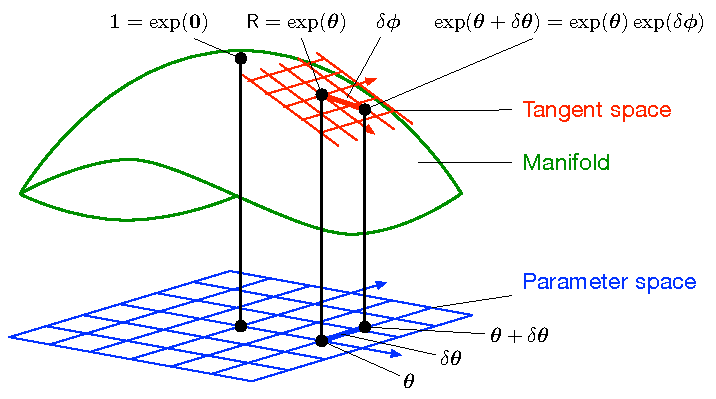
\includegraphics{figures/right_jac}
\caption{右 Jacobian 矩阵 $\bfJ_r=\dparil{\delta\bfphi}{\delta\bftheta}$ 将参数 $\bftheta$ 周围的变量 $\delta\bftheta$ 映射进入变量 $\delta\bfphi$ 在向量空间与流形相切的点 $\Exp{\bftheta}$ 处。}
\label{fig:right_jac}
\end{center}
\end{figure}
%
这个 Jacobian 矩阵称为 $SO(3)$ 的右雅可比矩阵(right Jacobian),并被定义为,
%We define the right Jacobian of $SO(3)$ as, 
%
\begin{align}
\bfJ_r(\bth) &\te \dpar{\Exp(\bth)}{\bth} 
~.
\end{align}
%
它的表达式独立于所使用的参数化,尽管它确实可以特别针对每个参数化来表示。使用方程 \eqRef{equ:dif_RtoSO3} 我们有,
%
\begin{align}
\bfJ_r(\bth) &= \lim_{\dth\to0}\frac{\Exp(\bth+\dth)\ominus\Exp(\bth)}{\dth} \\
 &= \lim_{\dth\to0}\frac{\Log(\Exp(\bth)\tr\Exp(\bth+\dth))}{\dth} && \textrm{if using $\bfR$} \\
 &= \lim_{\dth\to0}\frac{\Log(\Exp(\bth)^*\ot\Exp(\bth+\dth))}{\dth} && \textrm{if using $\bfq$} 
 ~.
\end{align}
%

右 Jacobian 矩阵及其逆矩阵可以进行闭式计算 \citep[page 40]{CHIRIKJIAN-12},
%
\begin{align}
\bfJ_r(\bth) &= \bfI - \frac{1-\cos\nth}{\nth^2}\hatx{\bth} + \frac{\nth-\sin\nth}{\nth^3}\hatx{\bth}^2 \\
\bfJ_r\inv(\bth) &= \bfI + \frac12\hatx{\bth} + \left(\frac1{\nth^2} - \frac{1+\cos\nth}{2\nth\sin\nth}\right)\hatx{\bth}^2
\end{align}



$SO(3)$ 的右 Jacobian 具有以下性质,对于任何 $\bth$ 和小的 $\dth$,
%
\begin{align}
\Exp(\bth+\dth) &\approx \Exp(\bth)\Exp(\bfJ_r(\bth)\dth) \label{equ:Jr1} \\
\Exp(\bth)\Exp(\dth) &\approx \Exp(\bth+\bfJ_r\inv(\bth)\,\dth) \\
\Log(\Exp(\bth)\Exp(\dth)) &\approx \bth+\bfJ_r\inv(\bth)\,\dth 
\end{align}


%-------------------------------------------------------------
\subsubsection{相对于旋转向量的 Jacobian 矩阵}

向量 $\bfa'=\bfR\{\bftheta\}\,\bfa$ 的旋转相对于旋转向量 $\bth$ 是一个从 $\bbR^3$ 到 $\bbR^3$ 的函数。它相对于旋转向量 $\bftheta$ 的导数使用方程 \eqRef{equ:derivative_vector} 并根据先前的结果扩展而来,使用方程 \eqRef{equ:Jr1},
%
\begin{align*} 
\dpar{(\bfq\ot\bfa\ot\bfq^*)}{\delta\bftheta} 
= \dpar{(\bfR\,\bfa)}{\delta\bftheta} 
&= \lim_{\delta\bftheta\to 0} \frac{\bfR\{\bftheta+\delta\bftheta\}\,\bfa-\bfR\{\bftheta\}\,\bfa}{\delta\bftheta} &&\gets\eqRef{equ:derivative_vector}\\
&= \lim_{\delta\bftheta\to 0} \frac{(\bfR\{\bftheta\}\Exp(\bfJ_r(\bftheta)\,\delta\bftheta)-\bfR\{\bftheta\})\bfa}{\delta\bftheta} && \gets\eqRef{equ:Jr1} \\
&= \lim_{\delta\bftheta\to 0} \frac{(\bfR\{\bftheta\}(\bfI+\hatx{\bfJ_r(\bftheta)\,\delta\bftheta})-\bfR\{\bftheta\})\bfa}{\delta\bftheta} \\
&= \lim_{\delta\bftheta\to 0} \frac{\bfR\{\bftheta\}\hatx{\bfJ_r(\bftheta)\,\delta\bftheta}\bfa}{\delta\bftheta} \\
&= \lim_{\delta\bftheta\to 0} -\frac{\bfR\{\bftheta\}\hatx{\bfa}\bfJ_r(\bftheta)\,\delta\bftheta}{\delta\bftheta} \\
&= -\bfR\{\bftheta\}\hatx{\bfa}\bfJ_r (\bftheta)
~,
\end{align*}
%
其中 $\bfR\{\bftheta\}\te\Exp(\bftheta)$。总结一下,
%
\begin{align} \label{equ:drot_da}
\eqbox{\dpar{(\bfq\ot\bfa\ot\bfq^*)}{\delta\bftheta} 
= \dpar{(\bfR\,\bfa)}{\delta\bftheta} 
= -\bfR\{\bftheta\}\hatx{\bfa}\bfJ_r(\bftheta) 
}~.
\end{align}


%-------------------------------------------------------------
\subsubsection{旋转组合的 Jacobians 矩阵}

考虑到 $SO(3)$ 的组合 $\sP=\sQ\circ\sR$,它可以以四元数或矩阵的形式实现,
%
\begin{align*}
\bfp &= \bfq_\theta\ot\bfr_\phi & \bfP &= \bfQ_\theta\,\bfR_\phi
\end{align*}
%
其中下标表示切空间中向量扰动的名字。 
这些是 从 $SO(3)$ 到 $SO(3)$的函数,因此我们使用方程 \eqRef{equ:derivative_SO3} 来写出导数,
%
\begin{align*}
\dpar{\sQ\circ\sR}{\sQ} 
= \dpar{\bfq_\theta\ot\bfr_\phi}{\bth} 
= \dpar{\bfQ_\theta \bfR_\phi}{\bth} 
&= \lim_{\delta\bftheta\to 0}\frac{((\bfQ_\theta\oplus\dth)\bfR_\phi)\ominus(\bfQ_\theta\bfR_\phi)}{\dth} \\
&= \lim_{\delta\bftheta\to 0}\frac{\Log[(\bfQ_\theta\bfR_\phi)\tr(\bfQ_\theta\Exp(\dth)\bfR_\phi)]}{\dth} \\
&= \lim_{\delta\bftheta\to 0}\frac{\Log[\bfR_\phi\tr\Exp(\dth)\bfR_\phi]}{\dth} \\
&= \lim_{\delta\bftheta\to 0}\frac{\Log[\Exp(\bfR_\phi\tr\dth)]}{\dth} \\
&= \lim_{\delta\bftheta\to 0}\frac{\bfR_\phi\tr\dth}{\dth}  = \bfR_\phi\tr 
\end{align*}
%
\begin{align*}
\dpar{\sQ\circ\sR}{\sR} 
= \dpar{\bfq_\theta\ot\bfr_\phi}{\bfphi} 
= \dpar{\bfQ_\theta \bfR_\phi}{\bfphi} 
&= \lim_{\delta\bfphi\to 0}\frac{(\bfQ_\theta(\bfR_\phi\oplus\delta\bfphi))\ominus(\bfQ_\theta\bfR_\phi)}{\delta\bfphi} \\
&= \lim_{\delta\bfphi\to 0}\frac{\Log[(\bfQ_\theta\bfR_\phi)\tr(\bfQ_\theta\bfR_\phi\Exp(\delta\bfphi))]}{\delta\bfphi} \\
&= \lim_{\delta\bfphi\to 0}\frac{\Log[\Exp(\delta\bfphi)]}{\delta\bfphi} \\
&= \lim_{\delta\bfphi\to 0}\frac{\delta\bfphi}{\delta\bfphi}  = \bfI 
\end{align*}

%=============================================================
\subsection{扰动、不确定性、噪声}

%-------------------------------------------------------------
\subsubsection{局部扰动}

扰动方向 $\tilde{\bfq}$ 可表示为未扰动方向 $\bfq$ 与一个小的局部扰动 ${\Delta\bfq_\cL}$ 的组合。 
因为 Hamilton 约定,该局部扰动出现在组合乘积的右手侧(\emph{right hand side}) --- 我们也给出了用于比较的等效矩阵,
%
\begin{align}
\tilde{\bfq} &= \bfq\ot{\Delta\bfq_\cL}
~, &
\tilde\bfR &= \bfR\,\Delta\bfR_\cL
~.
\end{align}%
%
使用指数映射,这些局部扰动 $\Delta\bfq_\cL$ (或 $\Delta\bfR_\cL$) 很容易从切空间中定义的等效向量形式 $\Delta\bfphi_\cL=\bfu\Delta\phi_\cL$ 获得。这给了
%
\begin{align}
\tilde\bfq_\cL &= \bfq_\cL\ot\Exp(\Delta\bfphi_\cL)
~,& 
\tilde\bfR_\cL &= \bfR_\cL\tdot\Exp(\Delta\bfphi_\cL)
\end{align}
%
导致局部扰动的表达式 
%
\begin{align}
\Delta\bfphi_\cL = \Log(\bfq_\cL^*\ot\tilde\bfq_\cL) = \Log(\bfR_\cL\tr\tdot\tilde\bfR_\cL)
\end{align}
 

如果扰动角度 $\Delta\phi_\cL$ 较小,则四元数和旋转矩阵形式的扰动可以由方程 \eqRef{equ:vectoquat} 和 \eqRef{equ:vectomat} 的泰勒展开近似到线性项,
%
\begin{align}
{\Delta\bfq_\cL}& \approx \begin{bmatrix}
1\\\frac{1}{2}\Delta\bfphi_\cL
\end{bmatrix}
~,
&
\Delta\bfR_\cL& \approx
\bfI+\hatx{\Delta\bfphi_\cL}
~.
\end{align}%
%
因此,扰动可以被指定为在局部向量空间 $\Delta\bfphi_\cL$ 相切于在与实际方向上的 $SO(3)$ 的流形。这是很方便的,例如,在这个向量空间中表示这些扰动的协方差矩阵,也就是说,使用规则的 $3\times 3$ 协方差矩阵。

\subsubsection{全局扰动}

考虑全局定义的扰动是可能的,而且确实有趣,对于相关的导数也是如此。 
全局扰动出现在组合乘积的左手侧(\emph{left hand side}),即,
%
%\begin{align}
%\tilde\bfq &= \Delta\bfq_\cG\otimes\bfq~, 
%&
%\tilde\bfR &= \Delta\bfR_\cG\,\bfR~.
%\end{align}
%
\begin{align}
\tilde\bfq_\cG &= \Exp(\Delta\bfphi_\cG)\ot\bfq_\cG
~,& 
\tilde\bfR_\cG &= \Exp(\Delta\bfphi_\cG)\tdot\bfR_\cG
\end{align}
%
导致全局扰动的表达式 
%
\begin{align}
\Delta\bfphi_\cG = \Log(\tilde\bfq_\cG\ot\bfq_\cG^*) = \Log(\tilde\bfR_\cG\tdot\bfR_\cG\tr)
\end{align}


同样,这些扰动可以被指定为在向量空间 $\Delta\bfphi_\cG$ 相切于在原点处的 $SO(3)$ 的流形。

\subsection{时间导数}

在向量空间中表示局部扰动,我们可以很容易地得到时间导数的表达式。 
只需将 $\bfq=\bfq(t)$ 作为初始状态,将 $\tilde{\bfq}=\bfq(t+\Dt)$ 作为扰动状态,并将导数的定义应用
%
\begin{align}
\dif{\bfq(t)}{t} \triangleq \lim_{\Dt\to0} \frac{\bfq(t+\Dt)-\bfq(t)}{\Dt}~, \label{equ:derivative}
\end{align}%
%
对上面,还有
%
\begin{align}
\bfomega_\cL(t) \triangleq \dif{\bfphi_\cL(t)}{t} \triangleq \lim_{\Dt\to0} \frac{\Delta\bfphi_\cL}{\Dt}~,
\end{align}%
%
其中,做为 $\Delta\bfphi_\cL$ 它是一个局部角扰动,对应于由 $\bfq$ 定义的局部坐标系中的角速率向量。

四元数时间导数的扩展如下 (旋转矩阵将使用类似的推理)
%
%
\begin{align}
\dot{\bfq} &\triangleq \lim_{\Dt\to0} \frac{\bfq(t+\Dt)-\bfq(t)}{\Dt} \nonumber\\
&= \lim_{\Dt\to0} \frac{\bfq\ot{\Delta\bfq_\cL}-\bfq}{\Dt} \nonumber\\
&= \lim_{\Dt\to0} \frac{\bfq\ot\left(\begin{bmatrix}
1\\\Delta\bfphi_\cL/2
\end{bmatrix}-\begin{bmatrix}
1\\\bf0
\end{bmatrix}\right)}{\Dt} \nonumber\\ 
&= \lim_{\Dt\to0} \frac{\bfq\ot\begin{bmatrix}
0\\\Delta\bfphi_\cL/2
\end{bmatrix}}{\Dt} \nonumber\\ 
&= \frac12\,\bfq\ot\begin{bmatrix}
0\\\bfomega_\cL
\end{bmatrix}
~. \label{equ:lastquatdev}
\end{align}%
%
定义
%
\begin{align}
\bfOmega(\bfomega) 
\triangleq \QR{\bfomega} 
= \begin{bmatrix}
0 & -\bfomega\tr \\
\bfomega & -\hatx{\bfomega}
\end{bmatrix} = \begin{bmatrix}
0        & -\omega_x & -\omega_y & -\omega_z \\
\omega_x & 0         &  \omega_z & -\omega_y \\
\omega_y & -\omega_z & 0         & \omega_x \\
\omega_z &  \omega_y & -\omega_x & 0
\end{bmatrix} ~, \label{equ:Omega}
\end{align}%
%
我们从方程 \eqRef{equ:lastquatdev} 和 \eqRef{equ:quatMatProd} 得到了 (我们也给出了它的等价矩阵)
%
\begin{empheq}[box=\widefbox]{align}
\label{equ:qdotLocal}
\dot{\bfq} &= \frac{1}{2}\bfOmega(\bfomega_\cL)\,\bfq = \frac{1}{2}\bfq\ot\bfomega_\cL
~,
&
\dot\bfR &= \bfR\hatx{\bfomega_\cL}
~.
\end{empheq}

这些表达式当然与方程 \eqRef{equ:qdot} 和 \eqRef{equ:Rdot}相同,是在旋转群 $SO(3)$ 的框架下发展起来的。 
然而,在这里,有趣的是,我们能够清楚地将角速率 $\bfomega_\cL$ 参考到一个特定的参考系,在这种情况下,该参考系是由方向 $\bfq$ 或 $\bfR$定义的局部坐标系。
这现在是可能的,因为我们已经给了算子 $\bfq$ 和 $\bfR$ 一个精确的几何意义。
从这个观点来看,方程 \eqRef{equ:qdotLocal} 表示当角速率在这个坐标系中的局部表示时,参考坐标系的方向的演变。

%-------------------------------------------------------------

与整体扰动相关的时间导数来自类似于方程 \eqRef{equ:lastquatdev}的扩展,其结果是
%
\begin{empheq}[box=\widefbox]{align}
\label{equ:qdotGlobal}
\dot\bfq &= \frac12\,\bfomega_\cG\ot\bfq~,
&
\dot\bfR &= \hatx{\bfomega_\cG}\bfR~,
\end{empheq}
%
其中
%
\begin{align}
\bfomega_\cG(t)\triangleq\dif{\bfphi_\cG(t)}{t}
\end{align}
%
是在全局坐标系中表示的角速率向量。
方程~\eqRef{equ:qdotGlobal}表示当角速率在全局参考坐标系中表示时,参考坐标系的方向的演变。
%-------------------------------------------------------------
\subsubsection{全局到局部(Global-to-local)的关系}

从上一段中,值得注意的是,局部角速率和全局角速率之间存在以下关系,
%
\begin{align}
\frac12\,\bfomega_\cG\ot\bfq = \dot\bfq = \frac12\,\bfq\ot\bfomega_\cL ~.
\end{align}
%
然后,后乘共轭四元数,我们有
%
\begin{align}
\bfomega_\cG = \bfq\ot\bfomega_\cL\ot\bfq^* = \bfR\,\bfomega_\cL~.
\end{align}
%
同样地,考虑到 $\Delta\bfphi_R \approx \bfomega\Dt$ 对于较小的 $\Dt$,我们有这些
%
\begin{align}
\Delta\bfphi_\cG = \bfq\ot\Delta\bfphi_\cL\ot\bfq^* = \bfR\,\Delta\bfphi_\cL~.
\end{align}
%
也就是说我们可以使用四元数或旋转矩阵,通过坐标系变换来变换角速率向量 $\bfomega$ 和小角度扰动 $\Delta\bfphi$ ,就好像它们是正则向量一样。同样可以通过姿态 $\bfomega=\bfu\omega$,或 $\Delta\bfphi=\bfu\Delta\phi$来理解,并且注意到旋转轴向量 $\bfu$ 正常地变换,用
% 
\begin{align}
\bfu_\cG=\bfq\ot\bfu_\cL\ot\bfq^*=\bfR\,\bfu_\cL ~.
\end{align}



%-------------------------------------------------------------
\subsubsection{四元数乘积的时间导数}

我们用正则公式求出乘积的导数,
%
\begin{align}
\dot{({\bfq_1\ot\bfq_2})} &= \dot{\bfq_1}\ot{\bfq_2} + \bfq_1\ot\dot{{\bfq_2}}~, 
&
\dot{(\bfR_1\bfR_2)} &= \dot\bfR_1\bfR_2+\bfR_1\dot\bfR_2~,
\end{align}%
%
但是要注意,由于乘积是非交换的,我们需要严格遵守操作数的顺序。
这意味着 $\dot{(\bfq^2)}\neq2\,\bfq\ot\dot\bfq
$~,就像标量情况一样,但是
%
\begin{align}
\dot{(\bfq^2)} = \dot\bfq\ot\bfq + \bfq\ot\dot\bfq 
%= \frac12\,\bfq\ot(\bfomega\ot\bfq+\bfq\ot\bfomega)
~.
\end{align}


%-------------------------------------------------------------
\subsubsection{其它有用的导数表达式}

我们可以导出局部旋转率的表达式
%
\begin{align}
\bfomega_\cL &= 2\,\bfq^*\ot\dot{\bfq}~, 
&
\hatx{\bfomega_\cL} &= \bfR\tr\,\dot\bfR~.
\end{align}%
%
以及全局自转率,
%
\begin{align}
\bfomega_\cG &= 2\,\dot{\bfq}\ot\bfq^*~, 
&
\hatx{\bfomega_\cG} &= \dot\bfR\,\bfR\tr~.
\end{align}%




%=============================================================
\subsection{转速的时间积分}

四元数形式的累积旋转是通过积分适合于旋转速率定义的微分方程来完成的,即,方程 \eqRef{equ:qdotLocal} 用于局部旋转速率定义,而方程 \eqRef{equ:qdotGlobal} 用于全局旋转速率定义。 
在我们感兴趣的情况下,角速率由局部传感器测量,从而在离散时间 $t_n=n\Dt$ 里提供局部测量 $\bfomega(t_n)$ 。
我们仅在此集中讨论这种情况,对于这种情况,我们再现微分方程 \eqRef{equ:qdotLocal},
%
\begin{align}
\dot\bfq(t) 
= \frac12\bfq(t)\ot\bfomega(t) 
~.
\label{equ:intLocal}
\end{align}

我们扩展了零阶和一阶积分方法,参见图(\ref{fig:quatInt} 和 \ref{fig:integrate}),都是在时间 $t=t_n$ 左右,基于 $\bfq(t_n+\Dt)$ 的泰勒级数。 
我们注意到 $\bfq\triangleq\bfq(t)$ 和 $\bfq_n\triangleq\bfq(t_n)$,并且对 $\bfomega$ 也一样。 
%
泰勒级数显示, 
%
\begin{align}
\q_{n+1} = \q_n + \dq_n\Dt + \frac1{2!}\ddq_n\Dt^2 + \frac1{3!}\dddq_n\Dt^3 + \frac1{4!}\ddddq_n\Dt^4 + \cdots~.
\label{equ:qnTaylor}
\end{align}
%
通过反复应用四元数导数方程 \eqRef{equ:intLocal},取 $\ddot\bfomega=0$,上述 $\bfq_n$ 的连续导数很容易得到。我们得到
%
\begin{subequations}
%
\begin{align}
\dq_n 
\e \frac12\q_n\w_n \\
\ddq_n 
\e \frac1{2^2}\q_n\w_n^2+\frac12\q_n\dw \\
\dddq_n 
\e \frac1{2^3}\q_n\w_n^3 + \frac14\q_n\dw\w_n + \frac12\q\w_n\dw \\
\q_n^{(i\,\ge\,4)} 
\e \frac1{2^i}\q_n\w_n^i + \cdots~,
\end{align}%
\label{equ:qnDerivatives}%
\end{subequations}%
%
这里我们为了节省符号而省略了 $\ot$ 的符号,也就是说,所有的 $\w$ 的乘积和幂必须用四元数乘积来解释。

\begin{figure}[tb]
\centering
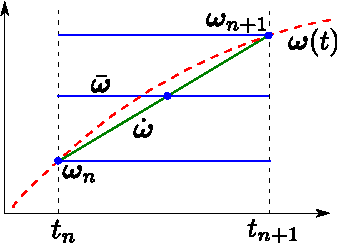
\includegraphics{figures/integral}
\caption{积分的角速度近似:红色:真实速度。蓝色:零阶近似 (下到上:前、中、后). 绿色:一阶近似。}
\label{fig:quatInt}
\end{figure}

\begin{figure}[tb]
\begin{center}
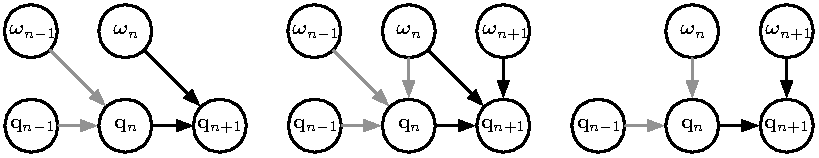
\includegraphics{figures/integrate}
\caption{两个连续时间步 (灰色和黑色箭头集合)的积分方案,其中共享相同时间戳的变量被组织成列。左:前向积分。中心:中间和一阶积分。右图:后向积分。}
\label{fig:integrate}
\end{center}
\end{figure}


%-------------------------------------------------------------
\subsubsection{零阶积分}


\paragraph{前向积分}
在角速率 $\bfomega_n$ 在周期 $[t_n,t_{n+1}]$ 内保持不变的情况下, %with $\Dt=t_{n+1}-t_n$~, 
我们有 $\dot\bfomega=0$ 并且方程 \eqRef{equ:qnTaylor} 降阶为,
%
\begin{align}
\q_{n+1} = \q_n\ot\left(
1 
+ \frac12\bfomega_n\Dt 
+ \frac1{2!}\Big(\frac12\bfomega_n\Dt\Big)^2 
+ \frac1{3!}\Big(\frac12\bfomega_n\Dt\Big)^3 
%+ \frac1{4!}\Big(\frac12\bfomega_n\Dt\Big)^4 
+  \cdots \right)~,
\end{align}
%
在这里我们确定指数 $e^{\bfomega_n\Dt/2}$ 的泰勒级数方程 \eqRef{equ:pureQuatExpSeries} 。 
从
方程 \eqRef{equ:vectoquat} 可知,
这个指数对应于四元数,代表增量旋转 $\Delta\theta=\bfomega_n\Dt$ ,
%
\begin{align*}
e^{\bfomega\Dt/2} = \Exp(\bfomega\Dt) = \bfq\{\bfomega\Dt\} = \begin{bmatrix}
\cos(\norm{\bfomega}\Dt/2) \\
\frac{\bfomega}{\norm{\bfomega}}\sin(\norm{\bfomega}\Dt/2)
\end{bmatrix}~,
\end{align*}
%
因此,
%
\begin{align}
\eqbox{
\bfq_{n+1} = \bfq_n\ot\bfq\{\bfomega_n\Dt\} 
} 
~.
\label{equ:intZeroth}
\end{align}


\paragraph{后向积分}
我们还可以认为,周期 $\Dt$ 上的恒定速度对应于 $\bfomega_{n+1}$,周期结束时测量的速度。这可以用类似的方式扩展,在 $t_{n+1}$ 附近用 $\bfq_n$ 的泰勒展开,导致
%
\begin{align}
{\bfq_{n+1} \approx \bfq_n\ot\bfq\{\bfomega_{n+1}\Dt\}} ~.
\end{align}

这里我们要指出的是,当到达的运动测量要实时处理时,这是典型的积分方法,因为积分视界对应于最后的测量 (在这种情况下, $t_{n+1}$,参见 \figRef{fig:integrate})。为了使这一点更加突出,我们可以重新标记时间索引,使用 $\{n-1,n\}$ 而不是 $\{n,n+1\}$,然后写,
%
\begin{align}
\eqbox{\bfq_n = \bfq_{n-1}\ot\bfq\{\bfomega_n\Dt\}} ~.
\end{align}

\paragraph{中间积分}

类似地,如果速度被认为在周期 $\Dt$ 的中间速率恒定(这不是周期中点的速度所必需的),
%
\begin{align}
\aw = \frac{\w_{n+1}+\w_n}{2}~,
\label{equ:wbar}
\end{align}
%
我们有,
%
\begin{align}
\eqbox{
\q_{n+1} = \bfq_n\ot\bfq\{\aw\Dt\} 
}
~.
\label{equ:intFirstC}
\end{align}

%-------------------------------------------------------------
\subsubsection{一阶积分}



角速率 $\w(t)$ 现在与时间成线性关系。它的一阶导数是常数,所有的高阶导数都是零,
%
%
\begin{align}
\dw \e \frac{\w_{n+1}-\w_n}{\Dt} \label{equ:wdot} \\
\ddot\w = \dddot\w = \cdots \e 0 \label{equ:wddot}
~.
\end{align}%
%
我们可以依据 $\w_n$ 和 $\dw$ 写出中间速率 $\aw$ ,
%
\begin{align}
\aw = \w_n+\frac12\dw\Dt~,
\end{align}
%
并依据更实用的 $\aw$ 和 $\dw$,导出出现在四元数导数方程 \eqRef{equ:qnDerivatives} 中的 $\w_n$ 的幂的表达式。
%
\begin{subequations}
%
\begin{align}
\w_n \e \aw-\frac12\dw\Dt \label{equ:wone}\\
\w_n^2 \e \aw^2 - \frac12\aw\dw\Dt - \frac12\dw\aw\Dt + \frac14\dw^2\Dt^2 \\
\w_n^3 \e \aw^3 - \frac32\aw^2\dw\Dt + \frac34\aw\dw^2\Dt^2 + \frac18\dw^3\Dt^3 \\
\w_n^4 \e \aw^4 + \cdots \label{equ:wthree}
~.
\end{align}%
\end{subequations}
%
将它们注入四元数导数,代入泰勒级数方程 \eqRef{equ:qnTaylor},经过适当的重排序后,我们有,
%
\begin{subequations}
%
\begin{align}
\q_{n+1} 
\e
\q\left(1+\frac12\aw\Dt+\frac1{2!}\left(\frac12\aw\Dt\right)^2+\frac1{3!}\left(\frac12\aw\Dt\right)^3+\cdots\right) \label{equ:exp} \\
&+\: \q\left(-\frac14\dw + \frac14\dw \right)\Dt^2 \label{equ:vanish}\\
&+\: \q\left(-\frac1{16}\aw\dw - \frac1{16}\dw\aw + \frac1{24}\dw\aw + \frac1{12}\aw\dw\right)\Dt^3 \label{equ:bracket} \\
&+\: \q\,\bigg(\:\cdots\:\bigg)\Dt^4 \:+\: \cdots 
\label{equ:neglected}
~,
\end{align}%
\end{subequations}
%
其中在方程 \eqRef{equ:exp} 中,我们识别到指数级数 $e^{\aw\Dt/2}= \q\{\aw\Dt\}$ ,方程 \eqRef{equ:vanish} 消失,并且方程 \eqRef{equ:neglected} 表示我们将忽略高幂次项。 
%
这在简化后产生 (我们现在恢复正常的 $\ot$ 符号),
%
\begin{align}
\q_{n+1} = \q_n\ot\q\{\aw\Dt\} + \frac{\Dt^3}{48}\q_n\ot(\aw\ot\dw - \dw\ot\aw) + \cdots ~.
\end{align}
%
代入 $\dw$ 和 $\aw$ ,根据它们的定义方程 \eqRef{equ:wdot} 和 \eqRef{equ:wbar} ,我们得到,
%
\begin{align}
\q_{n+1} = \q_n\ot\q\{\aw\Dt\} + \frac{\Dt^2}{48}\q_n\ot(\w_n\ot\w_{n+1} - \w_{n+1}\ot\w_n) + \cdots ~,
\label{equ:intFirstA}
\end{align}
%
这是一个等价于 \citep{TRAWNY-05-QUAT}的结果,但使用 Hamilton 约定,并且四元数积形式而不是矩阵积形式。 
最后,由于 $\bfa_v\ot\bfb_v-\bfb_v\ot\bfa_v=2\,\bfa_v\tcross\bfb_v$,参见方程 \eqRef{equ:quatCommutatorPure},我们有另一种形式,
%
%\begin{align}
%\eqbox{\q_{n+1} \approx \bfq_n\ot\bfq\{\aw\Dt\} + \frac{\Dt^2}{24}\,\bfq_n\ot\begin{bmatrix}
%0\\\w_n\tcross\w_{n+1}
%\end{bmatrix}} 
%~,
%\label{equ:intFirstB}
%\end{align}
%%
%or even
%
\begin{align} \label{equ:intFirstB}
\eqbox{\q_{n+1} \approx \bfq_n\ot\left(\bfq\{\aw\Dt\} + \frac{\Dt^2}{24}\,\begin{bmatrix}
0\\\w_n\tcross\w_{n+1}
\end{bmatrix}\right)
}~.
\end{align}
%
在这个表达式中,加法的第一项是零阶中间积分方程 \eqRef{equ:intFirstC}。
第二项是一个二阶校正,它会消失,当 $\w_n$ 和 $\w_{n+1}$ 共线时,%
\footnote{从方程 \eqRef{equ:intFirstA} 还可以注意到,如果四元数乘积是可交换的,此项将总是(\emph{always})消失,而不会存在。}
即当旋转轴从 $t_n$ 到 $t_{n+1}$ 没有变化时 。


\paragraph{固定旋转轴情况}

让我们写出 $\bfomega(t)=\bfu(t)\,\omega(t)$ 并称 $\bfu$ 为旋转轴。
在恒定旋转轴 $\bfu(t) = \bfu$情况下,我们有 $\w_n\tcross\w_{n+1}=0$ 并因此,
%
\begin{align}\label{equ:first_order_constant_axis}
\q_{n+1} = \bfq_n\ot\bfq\{\bfu\,\ol\omega\,\Dt\}~.
\end{align}
%
事实上,这个结果对于不限于 $\bfomega(t)$ 一阶导数的情况是有趣的。
实际上,如果旋转轴是常数,旋转进入四元数的无穷小贡献可交换,即, 
%
$$\exp (\bfu\,\omega_1\,\delta t_1)\exp (\bfu\,\omega_2\,\delta t_2)=\exp (\bfu\,\omega_2\,\delta t_2)\exp (\bfu\,\omega_1\,\delta t_1)=\exp (\bfu\,(\omega_1\delta t_1 + \omega_2\delta t_2))~,$$ 
%
并且因此我们有特征值,
%
\begin{subequations}
\begin{align}
\q_{n+1} 
  &= \bfq_n\ot \exp\left(\frac{\bfu}2\,\int_{t_n}^{t_{n+1}}\omega(t)\,\dt\right) \\
  &= \bfq_n\ot \exp(\bfu\,\Delta\theta_n/2) \\
  &= \bfq_n\ot \bfq\{\bfu\,\Delta\theta_n\}~.
\end{align}
\end{subequations}
%
其中 $\Delta\theta_n = \int_{t_n}^{t_{n+1}} \omega(t)dt \in \bbR$ 为区间 $[t_n,t_{n+1}]$ 内旋转的总角度。


\paragraph{变化旋转轴情况}

显然,在方程 \eqRef{equ:intFirstB} 中加法的第二项通过 $\w_n\tcross\w_{n+1}\neq0$ 捕获变化的旋转轴对积分方向的影响。
对于它的实际应用,我们注意到给定通常的 IMU 采样时间 $\Dt\le0.01s$,并且由于惯性,通常的 $\w_n$ 和 $\w_{n+1}$ 为近似共线性,这个二阶项的值为 $10^{-6}\nw^2$ 阶,或容易变得更小。 
具有更高幂次的 $\w\Dt$ 的项甚至更小,并且被忽略。 


还请注意,虽然所有零阶积分器通过构造产生单位四元数 (因为它们是作为两个单位四元数的乘积计算的),但由于方程 \eqRef{equ:intFirstB} 中的加法,这不是一阶积分器的情况。因此,在使用一阶积分器时,即使所述的求和项很小,用户也应注意检查四元数范数随时间的演化,并最终在需要时使用形式 $\bfq\gets\bfq/\norm{\bfq}$的四元数更新来重新规范化四元数。只有当定轴假设成立时,则方程 \eqRef{equ:first_order_constant_axis} 也成立,而这种规范化不再是必要的。 




% !TEX root = kinematics.tex


%\clearpage
%%%%%%%%%%%%%%%%%%%%%%%%%%%%%%%%%%%%%%%%%%%%%%%%%%%%%%%%%%%%%%
\section{IMU驱动的系统的误差状态动力学}
\label{sec:es-kinematics}

%=============================================================
\subsection{动机}

我们希望使用 Hamilton 四元数来表示在空间或姿态(\emph{attitude})上的方向,写出惯性系统动力学的误差状态方程,输入数据为带有偏差和噪声的加速度计和陀螺仪的读数。

加速度计和陀螺仪的读数通常来自惯性测量单元 (IMU)。
集成 IMU 读数导致具有随时间漂移的航位推算定位系统。
避免漂移是将这些信息与绝对位置读数,如 GPS 或视觉数据,融合的问题。

误差状态 Kalman 滤波器 (ESKF) 是我们可以用于此目的的工具之一。 
在 Kalman 滤波范式中,这些是ESKF最显著的资产~\citep{MADYASTHA-11}:

\begin{itemize}
\item 方向误差状态最小 (即,其参数数量与自由度相同),避免了过度参数化 (或冗余) 的相关问题,以及相关协方差矩阵奇异性的风险,这通常是由强制约束引起的。
\item 误差状态系统总是在接近原点的位置运行,因此远离可能的参数奇异性、万向节锁问题,或类似的问题,从而提供保证在所有时间里线性化有效性始终保持不变。
\item 误差状态总是很小,这意味着所有二阶乘积都可以忽略不计。 
这使得 Jacobians 矩阵的计算变得非常简单和快速。 
有些 Jacobians 矩阵数值甚至可能是常数或等于可用状态量。
\item 误差动力学变化很慢,因为所有大信号动力学已集成在标称状态。这意味着我们可以以低于预测的速度应用 KF 修正 (这是观测误差的唯一方法)。
\end{itemize}


%=============================================================
\subsection{误差状态 Kalman 滤波器的解释}

在误差状态滤波器公式中,我们提到真实、标称和误差状态值,真实状态表示为标称和误差状态的适当组合 (线性加和、四元数积或矩阵积)。 
其思想是将标称状态视为大信号 (非线性可积),将误差状态视为小信号 (线性可积,适用于线性高斯滤波)。

误差状态过滤器可以解释如下。 
一方面,高频 IMU 数据 $\bfu_m$ 被集成到标称状态 $\bfx$中, 
该标称状态不考虑噪声项 $\bfw$ 和其它可能的模型缺陷。 
因此,它会累积误差。 
这些误差被收集进误差状态 $\delta\bfx$ 中并且用误差状态 Kalman 滤波器 (ESKF)进行估计,这时合并了所有的噪声和扰动。 
误差状态由小信号量组成,其演化函数由一个 (时变) 线性动力学系统正确定义,其动力学、控制和测量矩阵由标称状态值计算。 
与标称状态积分并行,ESKF 预测误差状态的高斯估计。 
它只是预测,因为到目前为止还没有其它的测量方法来修正这些估计。 
滤波器校正是在 IMU 以外的信息(例如GPS、视觉等)到达时执行的,该信息能够使误差变得可观测,并且通常以比积分阶段低得多的速率发生。 
这种校正提供了误差状态的后验高斯估计。 
在此之后,将误差状态的均值注入标称状态,然后重置为零。 
误差状态的协方差矩阵被方便地更新以反映这种重置。 
这个系统就一直这样循环下去。

%\begin{enumerate}
%\item Have nominal state $\bfx$, error state $\delta\bfx$, covariance of error state $\bfP$. Have:
%%    
%$$\bfx_t = \bfx \oplus \delta\bfx$$
%%
%the true state is a composition of the nominal state and the error state (see 5. below for details)
%\item  Time-Update. Update the nominal state
%%
%    $$\bfx = f(\bfx,\bfu,0)$$
%%
%    where
%        $f()$ is the dynamic function,
%        $\bfu$ is the control signal, and
%        $\bfn=0$ is the noise mean.
%\item  Time-Update. Update the covariance of the error state
%%
%    $$\bfP = \bfF_\bfx \bfP \bfF_\bfx\tr + \bfF_\bfn \bfQ \bfF_\bfn\tr$$
%%
%    where        $\bfF_\bfx = d f() / d \delta\bfx$   the derivative \wrt $\delta\bfx$,
%        $\bfF_\bfn = d f() / d \bfn$    the derivative \wrt $\bfn$, and
%        $\bfQ$ covariance of the perturbation noise
%\item Measurement-update. Compute the Kalman gain
%%
%    $$\bfK = \bfP \bfH' / (\bfH \bfP \bfH' + \bfR)$$
%%
%    where
%        $h()$ is the measurement function,
%        $\bfH = d h() / d \delta\bfx$    the derivative of the measurement function $h()$ \wrt the error state $\delta\bfx$, and
%        $\bfR$ = covariance of the measurement noise
%\item  Measurement-update. Compute the error state
%%
%    $$\delta\bfx = \bfK ( \bfy - h(\bfx) )$$
%%
%    where
%        $\bfy$ is the measurement, and
%        $h(\bfx)$ is the measurement function evaluated at the nominal state (computed in step 1)
%\item  Measurement-update. Update the nominal state
%    $$\bfx = \bfx \oplus \delta\bfx$$
%    where
%        $\oplus$ is a composition. As $\bfx = [\bfv~ \bfq]$ and $\delta\bfx = [\delta\bfv~ \delta\bftheta]$, we have two cases:
%            general vectors, $\bfv = \bfv + \delta\bfv$, and
%            quaternion, $\bfq = \delta\bfq \otimes \bfq$,
%                where
%                $\ot$ is the quaternion product, and
%                $\delta\bfq$ is obtained from $\delta\bftheta$ with \eqRef{equ:vectoquatEuler}.
%\item  Measurement-update. Update the covariance of the error state
%   $$ \bfP = \bfP - \bfK (\bfH \bfP \bfH\tr + \bfR) \bfK\tr$$
%\item  Return to 1.
%\end{enumerate}

%=============================================================
\subsection{连续时间的系统动力学}

所有相关变量的定义总结于 \tabRef{tab:errorstatevar}。
关于约定的两项重要决定值得一提:
\begin{itemize}
\item
角度速率 $\bfomega$ 是相对于标称四元数的局部(\emph{locally})定义。 
这使得我们可以直接使用陀螺仪测量值 $\bfomega_m$ ,因为它们提供机体参考角速率。
\item
角度误差 $\delta\bftheta$ 同样是相对于标称方向的局部(\emph{locally})定义。 
这不一定是最佳的方法,但它符合大多数 IMU 集成工作的选择 --- 我们可以称之为经典方法(\emph{classical approach})。 
现有的证据 \citep{LI-2012} 表明全局定义的角度误差具有更好的性质。 
本文档 \secRef{sec:ESKFglobal}也将对此进行探讨,但这里的大多数开发、示例和算法都基于这种局部定义的角度误差。
\end{itemize}

\begin{table*}[tb]
\renewcommand{\arraystretch}{1.3}
\caption{误差状态 Kalman 滤波器中的所有变量。}
\centering
\vspace{1ex}
\begin{tabular}{|l|c|c|c|c|c|c|}
\hline
数量 & 真实 & 标称 & 误差 & 组合 & 测量 & 噪声 \\
\hline
\hline
全状态 ($ ^1$)& $\bfx_t$ & $\bfx$ & $\delta\bfx$ & $\bfx_t = \bfx\oplus\delta\bfx$ & & \\
\hline
\hline
位置 & $\bfp_t$ & $\bfp$ & $\delta\bfp$ & $\bfp_t = \bfp+\delta\bfp$ & & \\
速度 & $\bfv_t$ & $\bfv$ & $\delta\bfv$ &$\bfv_t = \bfv+\delta\bfv$& & \\
四元数 ($ ^{2,3}$)& $\bfq_t$ & $\bfq$ & ${\delta\bfq}$ &$\bfq_t = \bfq\ot{\delta\bfq}$& & \\
旋转矩阵 ($ ^{2,3}$)& $\bfR_t$ & $\bfR$ & $\delta\bfR$ &$\bfR_t = \bfR\,\delta\bfR$& & \\
 \multirow{2}{*}{角度向量 ($ ^{4}$)} &  &  &  \multirow{2}{*}{$\delta\bftheta$} & 
$\delta\bfq = e^{\delta\bftheta/2} 
%	\approx \begin{bmatrix}1\\\delta\bftheta/2\end{bmatrix}
	$ & & \\
& & & & 
$\delta\bfR = e^{\hatx{\delta\bftheta}} 
%	\approx \bfI + \hatx{\delta\bftheta}
	$ & &\\
\hline 
加速度计偏差 & $\bfa_{bt}$ & $\bfa_b$ & $\delta\bfa_b$ &$\bfa_{bt} = \bfa_b+\delta\bfa_b$& & $\bfa_w$ \\
陀螺偏差 & $\bfomega_{bt}$ & $\bfomega_b$ & $\delta\bfomega_b$ &$\bfomega_{bt} = \bfomega_b+\delta\bfomega_b$& & $\bfomega_w$ \\
重力向量 & $\bfg_t$ & $\bfg$ & $\delta\bfg$ & $\bfg_t = \bfg+\delta\bfg$ & & \\
\hline\hline
加速度 & $\bfa_t$ & 
&&& $\bfa_m$ & $\bfa_n$ \\
角速率 & $\bfomega_t$ & 
&&& $\bfomega_m$ & $\bfomega_n$ \\
\hline
\multicolumn{7}{l}{($ ^1$) 符号 $\oplus$ 指示一般组合} \\
\multicolumn{7}{l}{($ ^2$) 指示非最小表示} \\
\multicolumn{7}{l}{($ ^3$) 全局定义角度误差的组合公式,参见 \tabRef{tab:local_to_global} }\\
\multicolumn{7}{l}{($ ^4$) 指数定义,参见方程 (\ref{equ:vectoquat}) 和 (\ref{equ:vectomat},\,\ref{equ:rodrigues})}
\end{tabular}
\label{tab:errorstatevar}
\end{table*}%


%-------------------------------------------------------------
%-------------------------------------------------------------
\subsubsection{真实状态动力学}

真实状态动力学是
%
\begin{subequations}
%
\begin{align}
\dot\bfp_t &= \bfv_t \\
\dot\bfv_t &= \bfa_t \\
\dot{\bfq_t} &= \frac{1}{2}\bfq_t\ot\bfomega_t \\
\dot\bfa_{bt} &= \bfa_w \\
\dot\bfomega_{bt} &= \bfomega_w \\
\dot\bfg_t &= 0
\end{align}%
\end{subequations}
%
这里,在机体坐标系中,从 IMU 中以带噪声的传感器读数 $\bfa_m$ 和 $\bfomega_m$ 的形式获得真实的加速度 $\bfa_t$ 和角速度 $\bfomega_t$ 。即\footnote{在旋转动力学中描述的方程 \eqRef{equ:gyroModel},通常忽略地球的旋转速率 $\bfomega_\cE$ ,否则将是 $\bfomega_m = \bfomega_t + \bfR_t\tr\bfomega_\cE + \bfomega_{bt} + \bfomega_n$。
在绝大多数实际情况下,考虑非零地球旋转速率是不合理的复杂。
然而,我们注意到,当使用高端 IMU 传感器时,噪声和偏差非常小,对地球旋转速率的值 $\omega_\cE=15^\circ$/h $\approx 7.3\cdot10^{-5}\,$rad/s ,可能会变得直接可测量;在这种情况下,为了保持 IMU 误差模型的有效性,在公式中这转速 $\bfomega_\cE$ 不应该被忽略。}
%
%
\begin{align}
\bfa_m &= \bfR_t\tr(\bfa_t - \bfg_t) + \bfa_{bt} + \bfa_n \\
\bfomega_m &= \bfomega_t + \bfomega_{bt} + \bfomega_n \label{equ:gyroModel}
\end{align}%
%
还有 $\bfR_t\triangleq\bfR\{\bfq_t\}$。这样,真实值就可以被分离出来 (这意味着我们已经将测量方程颠倒了),
%
%
\begin{align}
\bfa_t &= \bfR_t(\bfa_m - \bfa_{bt} - \bfa_n) + \bfg_t \\
\bfomega_t &= \bfomega_m - \bfomega_{bt} - \bfomega_n.
\end{align}%
%
代入上面的结果得到动力学系统
%
\begin{subequations}
%
\begin{align}
\dot\bfp_t &= \bfv_t \label{equ:pos} \\
\dot\bfv_t &= \bfR_t(\bfa_m - \bfa_{bt} - \bfa_n) + \bfg_t \label{equ:vel} \\
\dot{\bfq_t} &= \frac{1}{2}\bfq_t\ot(\bfomega_m - \bfomega_{bt} - \bfomega_n) \label{equ:quat}\\
\dot\bfa_{bt} &= \bfa_w \label{equ:abias}\\
\dot\bfomega_{bt} &= \bfomega_w \label{equ:wbias}\\
\dot\bfg_t &= 0 \label{equ:grav}
\end{align}%
\end{subequations}
%
我们可以把它命名为 $\dot\bfx_t=f_t(\bfx_t,\bfu,\bfw)$ 。 
这个系统具有状态 $\bfx_t$,由 IMU 带噪声的读数 $\bfu_m$控制,并受白高斯噪声 $\bfw$干扰,所有这些都定义为
%
\begin{equation}
\bfx_t = \begin{bmatrix}
\bfp_t \\ \bfv_t \\ \bfq_t \\ \bfa_{bt} \\ \bfomega_{bt} \\ \bfg_t
\end{bmatrix} 
\Quad
\bfu = \begin{bmatrix}
\bfa_m - \bfa_n \\ \bfomega_m - \bfomega_n
\end{bmatrix}
\Quad
\bfw = \begin{bmatrix}
\bfa_w \\ \bfomega_w
\end{bmatrix}~.
\end{equation}
%

\bigskip
需要注意的是,在上述公式中,重力向量 $\bfg_t$ 将由滤波器估计。 
它有一个常数演化方程 \eqRef{equ:grav},对应于已知为常数的量级。 
系统从一个固定且任意已知的初始方向 $\bfq_t(t=0)=\bfq_0$开始,该初始方向通常不在水平面上,这使得初始重力向量通常未知。 
为了简单起见,通常取 $\bfq_0=(1, 0, 0, 0)$ 并因此 $\bfR_0=\bfR\{\bfq_0\}=\bfI$ 。 
我们估计在坐标系 $\bfq_0$ 中表示的 $\bfg_t$ ,而不是在水平坐标系中表示的 $\bfq_t$ ,以便将方向上的初始不确定度转换为重力方向上的初始不确定度。 
我们这样做是为了改善线性:事实上,方程 \eqRef{equ:vel} 现在在 $\bfg$中是线性的,它携带了所有的不确定性,并且初始方向 $\bfq_0$ 是已知的,没有不确定性,因此 $\bfq$ 开始时没有不确定性。 
一旦估计了重力向量,水平面就可以恢复,如果需要,整个状态和恢复的运动轨迹就可以重新定向,以反映估计的水平面。 
更多理由参见 \citep{LUPTON-09} 。 
这当然是可选的,读者可以自由地从系统中删除所有与重力相关的方程,并采用更经典的方法考虑 $\bfg\triangleq(0,0,-9.8xx)$,其中 $xx$ 是实验现场重力向量的适当小数位数,且初始方向 $\bfq_0$ 不确定。



%-------------------------------------------------------------
\subsubsection{标称状态动力学}

标称状态动力学对应于无噪声或扰动的建模系统,
%
\begin{subequations}
%
\begin{align}
\dot\bfp &= \bfv \label{equ:pdot}\\
\dot\bfv &= \bfR(\bfa_m - \bfa_b) + \bfg \label{equ:vdot}\\
\dot{\bfq} &= \frac{1}{2}\bfq\ot(\bfomega_m - \bfomega_b) \\
\dot\bfa_b &= 0 \\
\dot\bfomega_b &= 0 \\
\dot\bfg &= 0 .
\end{align}%
\end{subequations}
%




%-------------------------------------------------------------
\subsubsection{误差状态动力学}

目标是确定误差状态的线性化动力学。 
对于每个状态方程,我们写下其组合 (在 \tabRef{tab:errorstatevar}),求解误差状态并简化所有二阶无穷小。 
我们在这里给出了全误差状态动力学系统,并进行了评述和证明。
%
\begin{subequations}\label{equ:efull}
%
\begin{align}
\dot{\delta\bfp} &= \delta\bfv \label{equ:epos}\\
\dot{\delta\bfv} &= -\bfR\hatx{\bfa_m-\bfa_b}\delta\bftheta - \bfR\delta\bfa_b + \delta\bfg - \bfR\bfa_n \label{equ:evel}\\
\dot{\delta\bftheta} &= -\hatx{\bfomega_m-\bfomega_b}\delta\bftheta - \delta\bfomega_b - \bfomega_n \label{equ:equat}\\
\dot{\delta\bfa_b} &= \bfa_w \label{equ:eabias}\\
\dot{\delta\bfomega_b} &= \bfomega_w \label{equ:ewbias}\\
\dot{\delta\bfg} &= 0 .\label{equ:egrav}
\end{align}%
\end{subequations}
%
方程 \eqRef{equ:epos}, \eqRef{equ:eabias}, \eqRef{equ:ewbias} 和 \eqRef{equ:egrav},分别是位置、两个偏差和重力误差,从线性方程组导出,并且它们的误差状态动力学是平凡的。 
作为一个例子,考虑真实和标称位置方程 \eqRef{equ:pos} 和 \eqRef{equ:pdot},从 \tabRef{tab:errorstatevar} 中可知它们的组合 $\bfp_t=\bfp+\delta\bfp$ ,并求解 $\dot{\delta \bfp}$ 以获得 \eqRef{equ:epos}。

速度方程 \eqRef{equ:evel} 和方向误差方程 \eqRef{equ:equat},需要对非线性方程 \eqRef{equ:vel} 和 \eqRef{equ:quat} 进行一些非平凡的操作,以获得线性化动力学% of the linear velocity error $\delta\bfv$ and the angular error $\delta\bftheta$
。 
它们的证明在以下两个部分中展开。


\paragraph{方程 \eqRef{equ:evel}:线速度误差。}

我们希望确定 $\dot{\delta\bfv}$,速度误差的动力学。 
我们从以下关系开始
%
%
\begin{align}
\bfR_t &= \bfR(\bfI+\hatx{\delta\bftheta})  + O(\norm{\delta\bftheta}^2) \label{equ:Rt}\\
\dot\bfv &= \bfR\bfa_\cB + \bfg, \label{equ:vdot2}
\end{align}%
%
其中方程 \eqRef{equ:Rt} 是 $\bfR_t$的小信号近似,并且在方程 \eqRef{equ:vdot2} 中我们重写方程 \eqRef{equ:vdot} 但引入 $\bfa_\cB$ 和 $\delta\bfa_\cB$,定义为机体坐标系中的大信号和小信号加速度,
%
%
\begin{align}
\bfa_\cB &\triangleq \bfa_m - \bfa_b \label{equ:nomacc}\\
\delta\bfa_\cB &\triangleq -\delta\bfa_b - \bfa_n  \label{equ:pertacc}
\end{align}%
%
所以我们可以把惯性系中的真实加速度写成大、小信号项的组合,
%
\begin{equation}
\bfa_t = \bfR_t(\bfa_\cB+\delta\bfa_\cB) + \bfg + \delta\bfg.
\end{equation}%

我们以两种不同的形式 (左和右展开),继续写 $\dot\bfv_t$ 的表达式 \eqRef{equ:vel} ,其中 $O(\norm{\delta\bftheta}^2)$ 这项被忽略了,
%
%
\begin{align*}
\dot\bfv+\dot{\delta\bfv} =& \eqbox{\dot\bfv_t} = \bfR(\bfI+\hatx{\delta\bftheta})(\bfa_\cB+\delta\bfa_\cB)+\bfg + \delta\bfg \\
\bfR\bfa_\cB+\bfg+\dot{\delta\bfv} =&~~~~~~= \bfR\bfa_\cB+\bfR\delta\bfa_\cB+\bfR\hatx{\delta\bftheta}\bfa_\cB+\bfR\hatx{\delta\bftheta}\delta\bfa_\cB+\bfg+\delta\bfg 
\end{align*}%
%
将 $\bfR\bfa_\cB+\bfg$ 从左和右移动到
%
\begin{equation}
\dot{\delta\bfv} = \bfR(\delta\bfa_\cB+\hatx{\delta\bftheta}\bfa_\cB) + \bfR\hatx{\delta\bftheta}\delta\bfa_\cB + \delta\bfg
\end{equation}%
%
去掉二阶项,重新组织一些交叉积 (用 $\hatx{\bfa}\bfb=-\hatx{\bfb}\bfa$),我们得到
%
\begin{equation}
\dot{\delta\bfv} = \bfR(\delta\bfa_\cB - \hatx{\bfa_\cB}\delta\bftheta) + \delta\bfg,
\end{equation}%
%
然后,回顾方程 \eqRef{equ:nomacc} 和 \eqRef{equ:pertacc},
%
\begin{equation}
{\dot{\delta\bfv} = \bfR(-\hatx{\bfa_m-\bfa_b}\delta\bftheta - \delta\bfa_b - \bfa_n) + \delta\bfg}
\end{equation}%
%
在适当的重新排列后,会导致线速度误差的动力学变化,
%
\begin{equation}
\eqbox{\dot{\delta\bfv} = -\bfR\hatx{\bfa_m-\bfa_b}\delta\bftheta - \bfR\delta\bfa_b + \delta\bfg - \bfR\bfa_n}\ .
\end{equation}%
%
为了进一步澄清这个表达式,我们常常可以假设加速度计噪声是白色的、不相关的、各向同性的\footnote{如果三个 $XYZ$ 加速计不相同,则不能进行此假设。},
%
\begin{equation}
\bbE[\bfa_n] = 0 \Quad \bbE[\bfa_n\bfa_n\tr]=\sigma_a^2\bfI,
\end{equation}%
%
也就是说,协方差椭球是以原点为中心的球体,这意味着其均值和协方差矩阵在旋转时是不变的 (\emph{Proof:} $\bbE[\bfR\bfa_n] = \bfR\bbE[\bfa_n] = 0$ and $\bfE[(\bfR\bfa_n)(\bfR\bfa_n)\tr] = \bfR\bbE[\bfa_n\bfa_n\tr]\bfR\tr = \bfR\sigma_a^2\bfI\bfR\tr = \sigma_a^2\bfI$)。
然后我们可以重新定义加速度计的噪声向量,完全没有影响,根据
%
\begin{equation}
\bfa_n \gets \bfR\bfa_n
\end{equation}%
%
这给出
%
\begin{equation}
\eqbox{\dot{\delta\bfv} = -\bfR\hatx{\bfa_m-\bfa_b}\delta\bftheta - \bfR\delta\bfa_b + \delta\bfg - \bfa_n}\ .
\end{equation}%


\paragraph{方程 \eqRef{equ:equat}:方向误差。}


我们想确定 $\dot{\delta\bftheta}$,角度误差的动力学。我们从以下关系开始
%
%
\begin{align}
\dot{\bfq_t} &= \frac{1}{2}\bfq_t\ot\bfomega_t \\
\dot{\bfq} &= \frac{1}{2}\bfq\ot\bfomega ,
\end{align}%
%
这是四元数导数的真实定义和标称定义。

就像我们对加速度所做的那样,为了清晰起见,我们把大信号和小信号项按角度速率分组,
%
%
\begin{align}
\bfomega &\triangleq \bfomega_m - \bfomega_b \label{equ:nomangrate}\\
\delta\bfomega &\triangleq -\delta\bfomega_b - \bfomega_n, \label{equ:pertangrate}
\end{align}%
%
所以这个 $\bfomega_t$ 可以写为一个标称部分和一个误差部分,
%
\begin{equation}
\bfomega_t = \bfomega + \delta\bfomega .
\end{equation}%


我们用两种不同的方法(左和右展开)继续计算 $\dot{\bfq_t}$
%
%
\begin{align*}
\dot{{(\bfq\ot{\delta\bfq})}} =& \eqbox{\dot{\bfq_t}} = \frac{1}{2}\bfq_t\ot\bfomega_t \\
\dot{\bfq}\ot{\delta\bfq} + \bfq\ot\dot{{\delta\bfq}} =&~~~~~~= \frac{1}{2}\bfq\ot{\delta\bfq}\ot\bfomega_t \\
\frac{1}{2}\bfq\ot\bfomega\ot{\delta\bfq}+\bfq\ot\dot{{\delta\bfq}} =&& 
\end{align*}%
%
简化前导 $\bfq$ 和分离 $\dot{{\delta\bfq}}$ ,我们获得
%
%
\begin{align}
\begin{bmatrix}
0\\\dot{\delta\bftheta}
\end{bmatrix} = \eqbox{2\dot{{\delta\bfq}}} &= {\delta\bfq}\ot\bfomega_t - \bfomega\ot{\delta\bfq} \nonumber \\
&= [\bfq]_R(\bfomega_t){\delta\bfq} - [\bfq]_L(\bfomega){\delta\bfq} \nonumber \\
&= \begin{bmatrix}
0 & -(\bfomega_t-\bfomega)\tr \\
(\bfomega_t-\bfomega) & -\hatx{\bfomega_t+\bfomega} 
\end{bmatrix}\begin{bmatrix}
1 \\
\delta\bftheta/2
\end{bmatrix} + O(\norm{\delta\bftheta}^2) \nonumber \\
&= \begin{bmatrix}
0 & -\delta\bfomega\tr \\
\delta\bfomega & -\hatx{2\bfomega+\delta\bfomega} 
\end{bmatrix}\begin{bmatrix}
1 \\
\delta\bftheta/2
\end{bmatrix} + O(\norm{\delta\bftheta}^2) 
\end{align}%
%
结果是一个标量和一个向量等式
%
\begin{subequations}
%
\begin{align}
0 &= \delta\bfomega\tr\delta\bftheta + O(|\delta\bftheta|^2) \\
\dot{\delta\bftheta} &= \delta\bfomega - \hatx\bfomega\delta\bftheta - \frac{1}{2}\hatx{\delta\bfomega}\delta\bftheta + O(\norm{\delta\bftheta}^2).
\end{align}%
\end{subequations}
%
第一个方程导致 $\delta\bfomega\tr\delta\bftheta = O(\norm{\delta\bftheta}^2)$,这是由二阶无穷小形成的,不是很有用。 
第二个方程在忽略所有二阶项之后得到,
%
\begin{equation}
{\dot{\delta\bftheta} = -\hatx\bfomega\delta\bftheta} + \delta\bfomega 
\end{equation}%
%
并且最后,回顾方程 \eqRef{equ:nomangrate} 和 \eqRef{equ:pertangrate},我们得到了角度误差的线性化动力学,
%
\begin{equation}
\eqbox{\dot{\delta\bftheta} = -\hatx{\bfomega_m-\bfomega_b}\delta\bftheta - \delta\bfomega_b - \bfomega_n}\ .
\end{equation}%

%=============================================================
\subsection{离散时间系统动力学}

上面的微分方程需要积分到差分方程中,以考虑离散时间间隔 $\Dt>0$ 。
积分方法可能有所不同。 
在某些情况下,可以使用精确的闭式解。 
在其它情况下,可采用不同精度的数值积分。 
有关积分方法的相关详细信息,请参阅附录。

需要对以下子系统进行积分:
%
\begin{enumerate}
\item 标称状态。
\item 误差状态。
\begin{enumerate}
\item 确定性部分:状态动力学和控制。
\item 随机部分:噪声和扰动。
\end{enumerate}
\end{enumerate}

%-----------------------------------------------
%-------------------------------------------------------------
\subsubsection{标称状态动力学}

我们可以把标称状态的差分方程写为
%
\begin{subequations}
%
\begin{align}
\bfp &\gets \bfp + \bfv\, \Dt + \frac{1}{2}(\bfR(\bfa_{m}-\bfa_{b})+\bfg)\, \Dt ^2\\
\bfv &\gets \bfv + (\bfR(\bfa_{m}-\bfa_{b})+\bfg)\, \Dt \\
\bfq &\gets \bfq\ot \bfq\{(\bfomega_{m} - \bfomega_{b})\, \Dt\} \\
\bfa_{b} &\gets \bfa_{b} \\
\bfomega_{b} &\gets \bfomega_{b} \\
\bfg &\gets \bfg~,
\end{align}%
\end{subequations}%
%
根据方程 \eqRef{equ:vectoquat} ,其中, $x\gets f(x,\bullet)$ 表示类型为 $x_{k+1} = f(x_k,\bullet_k)$, $\bfR\triangleq\bfR\{\bfq\}$ 的时间更新是与当前标称方向 $\bfq$ 相关联的旋转矩阵,并且 $\bfq\{v\}$ 是与旋转 $v$ 相关联的四元数。

我们还可以使用更精确的积分,请参阅附录了解更多信息。



%===============================================
%-------------------------------------------------------------
\subsubsection{误差状态动力学}


确定性部分是正常积分的 (在这种情况下,我们遵循 \appRef{sec:BlockWiseTruncation} 中的方法。),同时随机部分的积分产生随机脉冲 (参见 \appRef{sec:IntNoise}),因此,
%
\begin{subequations}
%
\begin{align}
\delta\bfp &\gets \delta\bfp + \delta\bfv\,\Dt \\
\delta\bfv &\gets \delta\bfv + (-\bfR\hatx{\bfa_{m}-\bfa_{b}}\delta\bftheta - \bfR\delta\bfa_{b} + \delta\bfg)\Dt + \bfv_\bfi \\
\delta\bftheta &\gets \bfR\tr\{(\bfomega_{m}-\bfomega_{b})\Dt\}\delta\bftheta - \delta\bfomega_{b} \Dt + \bftheta_\bfi \\
\delta\bfa_{b} &\gets \delta\bfa_{b} + \bfa_\bfi \\
\delta\bfomega_{b} &\gets \delta\bfomega_{b} + \bfomega_\bfi \\
\delta\bfg &\gets \delta\bfg ~.
\end{align}%
\end{subequations}

这里, $\bfv_\bfi$, $\bftheta_\bfi$, $\bfa_\bfi$ 和 $\bfomega_\bfi$ 是应用于速度、方向和偏差估计的随机脉冲,由白色高斯过程建模。 
它们的均值为零,并且它们的协方差矩阵由在时间步 $\Dt$ 内的 $\bfa_n$, $\bfomega_n$, $\bfa_w$ 和 $\bfomega_w$ 的协方差的积分获得的  (参见 \appRef{sec:IntNoise}),
%
%
\begin{align}
\bfV_\bfi &= \sigma_{\tilde\bfa_n}^2\Dt^2\bfI \quad &&[m^2/s^2]\\
\Theta_\bfi &= \sigma_{\tilde\bfomega_n}^2\Dt^2\bfI \quad &&[rad^2] \\
\bfA_\bfi &= \sigma_{\bfa_w}^2\Dt\bfI \quad &&[m^2/s^4] \\
\bfOmega_\bfi &= \sigma_{\bfomega_w}^2\Dt\bfI \quad &&[rad^2/s^2] 
\end{align}%
%
其中, $\sigma_{\tilde\bfa_n}[m/s^2]$, $\sigma_{\tilde\bfomega_n}[rad/s]$, $\sigma_{\bfa_w}[m/s^2\sqrt{s}]$ 和 $\sigma_{\bfomega_w}[rad/s\sqrt{s}]$ 应根据 IMU 数据表中的信息或通过实验测量确定。



%-------------------------------------------------------------
\subsubsection{误差状态 Jacobian 矩阵和扰动矩阵}


Jacobians 矩阵是通过简单检查前一节中的误差状态差分方程得到的。 

为了以紧凑的形式编写这些方程,我们考虑标称状态向量 $\bfx$,误差状态向量 $\delta\bfx$,输入向量 $\bfu_m$,和扰动脉冲向量 $\bfi$,如下所示 (关于细节和理由,参见 \appRef{sec:pertImpulses}),
%
\begin{equation}
\bfx=\begin{bmatrix}\bfp\\\bfv\\\bfq\\\bfa_b\\\bfomega_b\\\bfg\end{bmatrix} \quad, \quad
\delta\bfx=\begin{bmatrix}\delta\bfp\\\delta\bfv\\\delta\bftheta\\\delta\bfa_b\\\delta\bfomega_b\\\delta\bfg\end{bmatrix} \quad, \quad
\bfu_m = \begin{bmatrix}
\bfa_m \\
\bfomega_m
\end{bmatrix} 
\quad,  \quad
\bfi = \begin{bmatrix}
\bfv_\bfi \\
\bftheta_\bfi \\
\bfa_\bfi \\
\bfomega_\bfi
\end{bmatrix}
\end{equation}


\bigskip
误差状态系统现在是
%
\begin{equation}
\delta\bfx \gets f(\bfx,\delta\bfx,\bfu_m,\bfi)=\bfF_\bfx(\bfx, \bfu_m)\tdot \delta\bfx+\bfF_\bfi\tdot\bfi,
\end{equation}
%
ESKF 预测方程写为:
%
%
\begin{align}
\hat{\delta\bfx} &\gets \bfF_\bfx(\bfx, \bfu_m)\tdot \hat{\delta\bfx} \label{equ:errorMeanPred} \\
\bfP &\gets \bfF_\bfx\,\bfP\,\bfF_\bfx\tr + \bfF_\bfi\,\bfQ_\bfi\,\bfF_\bfi\tr \label{equ:errorCovPred} ~,
\end{align}%
%
其中 $\delta\bfx\sim\cN\{\hat{\delta\bfx},\bfP\}$\footnote{$x\sim\cN\{\mu,\Sigma\}$ 意味着 $x$ 是一个高斯随机变量,其均值和协方差矩阵由 $\mu$ 和 $\Sigma$指定。}; $\bfF_\bfx$ 和 $\bfF_\bfi$ 是 $f()$ 的相对于误差和扰动向量的 Jacobians 矩阵;并且 $\bfQ_\bfi$ 是扰动脉冲的协方差矩阵。

Jacobian 矩阵和协方差矩阵的表达式如下所示。 
此处出现的所有与状态相关的值直接从标称状态中提取。
%
\begin{equation} \label{equ:Fx_local_euler}
\bfF_\bfx = \pjac{f}{\delta\bfx}{\bfx,\bfu_m} = \begin{bmatrix}
\bfI & \bfI\Dt & 0                             & 0               & 0                     & 0 \\
0 & \bfI    & -\bfR\hatx{\bfa_m-\bfa_b}\Dt     & -\bfR\Dt            & 0                     & \bfI\Dt \\
0 & 0    & \bfR\tr\{(\bfomega_m-\bfomega_b)\Dt\}   & 0               & -\bfI\Dt                  & 0 \\
0 & 0    & 0                             & \bfI & 0                     & 0 \\
0 & 0    & 0                             & 0               & \bfI  & 0 \\
0 & 0    & 0                             & 0               & 0                     & \bfI \\
\end{bmatrix}
\end{equation}%
%
\begin{equation}
\bfF_\bfi = \pjac{f}{\bfi}{\bfx,\bfu_m} = \begin{bmatrix}
0 & 0 & 0 & 0 \\
\bfI & 0 & 0 & 0 \\
0 & \bfI & 0 & 0 \\
0 & 0 & \bfI & 0 \\
0 & 0 & 0 & \bfI \\
0 & 0 & 0 & 0 
\end{bmatrix}  
\quad,\quad
\bfQ_\bfi = \begin{bmatrix}
\bfV_\bfi & 0        & 0      & 0 \\ 
0      & \bfTheta_\bfi & 0      & 0 \\ 
0      & 0        & \bfA_\bfi & 0 \\ 
0      & 0        & 0      & \bfOmega_\bfi 
\end{bmatrix}~.
\end{equation}%
%

请特别注意, $\bfF_\bfx$ 是系统的转换矩阵,它可以用不同的方式近似到不同的精度水平。 
我们在这里展示了它最简单的形式之一,欧拉形式 (Euler form)。
参阅附录 \ref{sec:ClosedFormInt} 到 \ref{sec:TranMatRK} 以供进一步参考。

还请注意,作为误差 $\delta\bfx$ 的均值,被初始化为零,线性方程 \eqRef{equ:errorMeanPred} 总是返回零。 
当然,你应该在你的代码中跳过方程 \eqRef{equ:errorMeanPred} 中的代码行。 
不过,我建议你把它写下来,但你把它注释掉,这样你才能确定你没有忘记任何事情。

最后,请注意,你不应该跳过协方差预测方程 \eqRef{equ:errorCovPred}!!实际上, $\bfF_\bfi\,\bfQ_\bfi\,\bfF_\bfi\tr$ 这些项不为空,并且因此协方差持续增长 --- 所以该方程必须处在任何预测步骤当中。


%\clearpage
%%%%%%%%%%%%%%%%%%%%%%%%%%%%%%%%%%%%%%%%%%%%%%%%%%%%%%%%%%%%%%
\section{互补传感数据与 IMU 融合}
\label{sec:fusion}

当 IMU 以外的其它信息,如 GPS 或视觉数据到达时,我们继续校正 ESKF。
在一个良好设计的系统中,这将使 IMU 的偏差可观测,并允许 ESKF 去正确估计它们。 
这里有很多种可能性,最流行的是 GPS + IMU,单目视觉 + IMU,和立体视觉 + IMU。 
近年来,视觉传感器与 IMU 的结合引起了人们的广泛关注,并由此产生了大量的科学研究。 
这些视觉 + IMU 设置对于在无 GPS 的环境中使用非常有趣,可以在移动设备 (通常是智能手机)上实现,也可以在无人机和其它小型、灵活的平台上实现。

\bigskip

虽然IMU信息到目前为止已用于对 ESKF 进行预测,但可其它信息用于校正滤波器,从而观测 IMU 偏差误差。 
校正包括三个步骤:
\begin{enumerate}
\item
 通过滤波器校正观测误差状态, 
\item
 将观测到的误差注入标称状态,并且
\item	
 重置误差状态。 
\end{enumerate}%
%
这些步骤将在以下章节中介绍。

%=============================================================
\subsection{通过滤波器校正观测误差状态}

像往常一样假设我们有一个传感器,它可以根据状态传递信息,比如
%
\begin{equation}
\bfy = h(\bfx_t) + v~,
\end{equation}
%
其中 $h()$ 是系统状态 (真实状态)的一般非线性函数,并且 $v$ 是协方差为 $\bfV$ 的白高斯噪声,
%
\begin{equation}
v\sim\cN\{0,\bfV\}~.
\end{equation}

我们的滤波器正在估计误差状态,因此滤波器校正方程\footnote{我们给出协方差更新的最简单形式, $\bfP \gets
 (\bfI-\bfK\bfH)\bfP$ 。 
众所周知,这种形式的数值稳定性较差,因为其结果不能保证对称或正定。 
读者可以自由使用更稳定的形式,如 1) 对称形式 $\bfP\gets\bfP-\bfK(\bfH\bfP\bfH\tr+\bfV)\bfK\tr$ 和 2) 对称和正 \emph{Joseph} 形式 $\bfP \gets (\bfI-\bfK\bfH)\bfP(\bfI-\bfK\bfH)\tr+\bfK\bfV\bfK\tr$ 。},
%
%
\begin{align}
\bfK &= \bfP\bfH\tr(\bfH\bfP\bfH\tr+\bfV)\inv \\
\hat{\delta\bfx} &\gets \bfK(\bfy-h(\hat\bfx_t)) \\
\bfP &\gets (\bfI-\bfK\bfH)\bfP
\end{align}%
%
要求 Jacobian 矩阵 $\bfH$ 相对于误差状态 $\delta\bfx$ 定义,并且在最佳真实状态估计 $\hat\bfx_t=\bfx\oplus\hat{\delta\bfx}$ 下进行评估。
由于现阶段的误差状态均值为零 (我们还没有观测到),我们有 $\hat\bfx_t = \bfx$ 并且我们可以使用标称误差 $\bfx$ 作为评估点,从而得出
%
\begin{equation}
\bfH \equiv \pjac{h}{\delta\bfx}{\bfx}~.
\end{equation}

%-------------------------------------------------------------
\subsubsection{滤波器校正的 Jacobian 矩阵计算}

上面的 Jacobian 矩阵可以用多种方法计算。 
最能说明问题的是利用链式规则, 
%
\begin{equation}
\bfH \triangleq \pjac{h}{\delta\bfx}{\bfx} 
= \pjac{h}{\bfx_t}{\bfx}\pjac{\bfx_t}{\delta\bfx}{\bfx} = \bfH_\bfx\ \bfX_{\delta\bfx}~.
\end{equation}
%
这里, $\bfH_\bfx\triangleq\pjac{h}{\bfx_t}{\bfx}$ 是 $h()$ 相对于其自身参数的标准 Jacobian 矩阵 (即,Jacobian 矩阵中的数值``1''可用于常规 EKF)。
链式规则的第一部分取决于所用特定传感器的测量功能,这里不介绍。 

第二部分,$\bfX_{\delta\bfx}\triangleq\pjac{\bfx_t}{\delta\bfx}{\bfx}$,是真实状态相对于误差状态的 Jacobian 矩阵。 
这一部分可以在这里推导出来,因为它只依赖于 ESKF 的状态组合。我们有导数,
%
\begin{equation}
\bfX_{\delta\bfx} = 
\begin{bmatrix}
\dpar{(\bfp+\delta\bfp)}{\delta\bfp} &&&&& \\ 
& \dpar{(\bfv+\delta\bfv)}{\delta\bfv} &&&0& \\ 
&& \dpar{(\bfq\otimes\delta\bfq)}{\delta\bftheta} &&& \\ 
&&& \dpar{(\bfa_b+\delta\bfa_b)}{\delta\bfa_b} && \\ 
&0&&& \dpar{(\bfomega_b+\delta\bfomega_b)}{\delta\bfomega_b} & \\ 
&&&&& \dpar{(\bfg+\delta\bfg)}{\delta\bfg} 
\end{bmatrix}
\end{equation}
%
这将导致所有特征值为 $3\times3$ 块 (例如, $\dpar{(\bfp+\delta\bfp)}{\delta\bfp}=\bfI_3$) 除了 $4\times3$ 的四元数项 $\bfQ_{\delta\bftheta} = \dparil{(\bfq\otimes\delta\bfq)}{\delta\bftheta}$。因此我们有了形式,
%
\begin{equation}
\bfX_{\delta\bfx}\triangleq\pjac{\bfx_t}{\delta\bfx}{\bfx} = \begin{bmatrix}
\bfI_6 & 0 & 0 \\
0 &  \bfQ_{\delta\bftheta} & 0 \\
0 & 0 & \bfI_9
\end{bmatrix}
\end{equation}


使用链式规则,方程 \eqsRef{equ:quatMatProd}{equ:quatMatrix},和 $\delta\bfq \underset{\delta\bftheta\to 0}{\longrightarrow} \begin{bmatrix}
1 \\ \frac12\delta\bftheta
\end{bmatrix}$ 的极限,四元数项 $\bfQ_{\delta\bftheta}$ 可导出如下,
%
{
\setlength{\arraycolsep}{2pt}
\begin{align*}
\bfQ_{\delta\bftheta} \triangleq \pjac{(\bfq\otimes\delta\bfq)}{\delta\bftheta}{\bfq} 
&=\pjac{(\bfq\otimes\delta\bfq)}{\delta\bfq}{\bfq} \pjac{\delta\bfq}{\delta\bftheta}{\hat{\delta\bftheta}=0} \\
&= \pjac{([\bfq]_L\delta\bfq)}{\delta\bfq}{\bfq} \pjac{\begin{bmatrix}
1 \\ \frac12\delta\bftheta
\end{bmatrix}}{\delta\bftheta}{\hat{\delta\bftheta}=0} \\
&= [\bfq]_L\,\frac12\begin{bmatrix}
0 & 0 & 0 \\
1 & 0 & 0 \\
0 & 1 & 0 \\
0 & 0 & 1 \\
\end{bmatrix} ~,
\end{align*}
%
这导致
%
\begin{equation}
\bfQ_{\delta\bftheta}
= \frac{1}{2}\begin{bmatrix}
-q_x &-q_y &-q_z\\
 q_w &-q_z & q_y\\
 q_z & q_w &-q_x\\
-q_y & q_x & q_w\\
\end{bmatrix}~.
\end{equation}•

%=============================================================
\subsection{将观测误差注入标称状态}

在 ESKF 更新之后,使用适当的组合 (四元数加法或乘积,参见 \tabRef{tab:errorstatevar}),
%
\begin{equation}
\bfx \gets \bfx \oplus \hat{\delta\bfx}~, \label{equ:errorInjection}
\end{equation}
%
也就是说,
%
\begin{subequations}
%
\begin{align}
\bfp &\gets \bfp + \hat{\delta\bfp} \\
\bfv &\gets \bfv + \hat{\delta\bfv} \\
\bfq &\gets \bfq \otimes \bfq\{\hat{\delta\bftheta}\} \label{equ:quatErrorInjection}\\
\bfa_b &\gets \bfa_b + \hat{\delta\bfa_b} \\
\bfomega_b &\gets \bfomega_b + \hat{\delta\bfomega_b} \\
\bfg &\gets \bfg + \hat{\delta\bfg} 
\end{align}%
\end{subequations}%

%=============================================================
\subsection{ESKF复位}

误差注入标称状态后,误差状态均值 $\hat{\delta\bfx}$ 被重置。 
这与方向部分特别相关,因为新的方向误差将是相对于新标称状态的方向坐标系的局部表示。 
为了使 ESKF 更新完成,需要根据此项修改更新误差的协方差。

\bigskip

让我们调用误差重置函数 $g()$ 。 
它是这样写为,
%
\begin{equation}
\delta\bfx \gets g(\delta\bfx) = \delta\bfx \ominus \hat{\delta\bfx}~, \label{equ:resetFcn}
\end{equation}
%
其中 $\ominus$ 代表 $\oplus$ 的组合的逆。
因此,ESKF 误差重置操作是,
%
\begin{align}
\hat{\delta\bfx} &\gets 0 \\
\bfP &\gets \bfG\,\bfP\,\bfG\tr~.
\end{align}
%
其中 $\bfG$ 是 Jacobian 矩阵,定义为,
%
\begin{equation}
\bfG \triangleq \pjac{g}{\delta\bfx}{\hat{\delta\bfx}}~.
\end{equation}

与上面的更新 Jacobian 矩阵类似,这个 Jacobian 矩阵是除方向误差之外的所有对角块上的特征矩阵。 
我们给出了完整的表达式,并在下一节中继续推导方向误差块, $\partial\delta\bftheta^+/\partial\delta\bftheta = \bfI - \hatx{\frac12\hat{\delta\bftheta}}$ ,
%
\begin{equation}
\bfG = \begin{bmatrix}
\bfI_6 & 0 & 0 \\
0 & \bfI - \hatx{\frac12\hat{\delta\bftheta}} & 0 \\
0 & 0 & \bfI_9
\end{bmatrix}~.
\end{equation}

在大多数情况下,误差项 $\hat{\delta\bftheta}$ 可以被忽略,直接导出 Jacobian 矩阵 $\bfG=\bfI_{18}$,从而导致一个平凡的误差重置。 
这就是 ESKF 的大多数实现所做的。
这里提供的表达式应该产生更精确的结果,这可能有助于减少里程计系统中的长期误差漂移。


%-------------------------------------------------------------
\subsubsection{相对于方向误差的重置操作的 Jacobian 矩阵}

我们要得到新的角度误差 $\delta\bftheta^+$ 相对于旧的误差 $\delta\bftheta$ 和观测误差 $\hat{\delta\bftheta}$ 的表达式。考虑以下事实:
\begin{itemize}
\item
在误差复位时,真实方向没有改变,即 $\bfq_t^+ = \bfq_t$。这就提供了:
%
\begin{equation}
\bfq^+\ot\delta\bfq^+ = \bfq\ot \delta\bfq~.
\end{equation}
%
\item
观测到的误差均值已注入标称状态 (参见方程 \eqRef{equ:quatErrorInjection} 和 \eqRef{equ:rotComposition}):
%
\begin{equation}
\bfq^+ = \bfq\ot \hat{\delta\bfq}~.
\end{equation}
\end{itemize}

结合这两个特征,我们得到 $\delta\bfq^+$ 的表达式,
%
\begin{equation}
\delta\bfq^+ 
= (\bfq^+)^* \ot \bfq \ot \delta\bfq 
= (\bfq \ot \hat{\delta\bfq})^* \ot \bfq \ot \delta\bfq 
= \hat{\delta\bfq}^* \ot \delta\bfq 
= [\hat{\delta\bfq}^*]_L\cdot\delta\bfq~.
\end{equation}
%
考虑到这点,
%
$\hat{\delta\bfq}^* \approx \begin{bmatrix}
1 \\ -\frac12\hat{\delta\bftheta}
\end{bmatrix}$,
%
上面的特征可以扩展为
%
\begin{equation}
\begin{bmatrix}
1 \\ \frac12\delta\bftheta^+
\end{bmatrix}
=
\begin{bmatrix}
1                  & \frac12\hat{\delta\bftheta}\tr \\
-\frac12\hat{\delta\bftheta} & \bfI - \hatx{\frac12\hat{\delta\bftheta}}
\end{bmatrix}
\cdot
\begin{bmatrix}
1 \\ \frac12\delta\bftheta
\end{bmatrix} + \cO(\norm{\delta\bftheta}^2) ~,
\end{equation}
%
它给出了一个标量方程和一个向量方程,
%
\begin{subequations}
%
\begin{align}
\frac14\hat{\delta\bftheta}\tr\delta\bftheta &= \cO(\norm{\delta\bftheta}^2)\\
\delta\bftheta^+ &= -\hat{\delta\bftheta} + \left(\bfI - \hatx{\frac12\hat{\delta\bftheta}}\right)\delta\bftheta + \cO(\norm{\delta\bftheta}^2)~,
\end{align}%
\end{subequations}
%
其中第一个并不是很有用,因为它只是无穷小的关系。 
从第二个方程可以看出 $\hat{\delta\bftheta}^+ = 0$,这是我们对复位操作的期望。 
Jacobian 矩阵通过简单的检验得到,
%
\begin{equation}
\eqbox{\dpar{\delta\bftheta^+}{\delta\bftheta} = \bfI - \hatx{\frac12\hat{\delta\bftheta}}}~.
\end{equation}


% !TEX root = kinematics.tex


%\clearpage
%%%%%%%%%%%%%%%%%%%%%%%%%%%%%%%%%%%%%%%%%%%%%%%%%%%%%%%%%%%%%%
\section{使用全局角度误差的 ESKF}
\label{sec:ESKFglobal}

在本节中,我们将探讨在全局参考中定义角度误差的含义,而不是我们目前使用的局部定义。 
我们回顾第 \ref{sec:es-kinematics} 节和第 \ref{sec:fusion} 节的发展,并详细说明了与新定义相关的变化。

全局定义的角度误差 $\delta\bftheta$ 意味着一个左手侧(\emph{left hand side})的组合,即,
%
\begin{equation*}
\bfq_t = \delta\bfq\ \ot \bfq = \bfq\{\delta\bftheta\} \ot \bfq~.
\end{equation*}

为了完备性,我们注意保持角度速率向量 $\bfomega$的局部定义,即在连续时间内 $\dot\bfq=\frac12\bfq\ot\bfomega$ ,并且因此在离散时间内 $\bfq \gets \bfq\ot\bfq\{\bfomega\Dt\}$ ,不考虑全局定义的角度误差。 
这是为了方便起见,因为陀螺仪提供的角度速率的测量是在机体内,也就是说,是局部的。

%=============================================================
\subsection{连续时间的系统动力学}

%-------------------------------------------------------------
\subsubsection{真实和标称状态动力学}

真实动力学和标称动力学不涉及误差,其方程不变。

%-------------------------------------------------------------
\subsubsection{误差状态动力学}

我们先写下误差状态动力学方程,并进行评论和证明。
%
\begin{subequations}\label{equ:efullglobal}
%
\begin{align}
\dot{\delta\bfp} &= \delta\bfv \label{equ:epglobal} \\
\dot{\delta\bfv} &= -\hatx{\bfR(\bfa_m-b\bfa_b)}\delta\bftheta - \bfR\delta\bfa_b + \delta\bfg - \bfR\bfa_n \label{equ:evglobal}\\
\dot{\delta\bftheta} &= -\bfR\delta\bfomega_b - \bfR\bfomega_n \label{equ:etglobal}\\
\dot{\delta\bfa_b} &= \bfa_w \label{equ:eabglobal}\\
\dot{\delta\bfomega_b} &= \bfomega_w \label{equ:ewbglobal}\\
\dot{\delta\bfg} &= 0 ~, \label{equ:egglobal}
\end{align}%
\end{subequations}%
%
这里, 再次的, 所有方程除了 $\dot{\delta\bfv}$ 和 $\dot{\delta\bftheta}$ 之外都是平凡的。 
非平凡表达式如下所示。


\paragraph{方程 \eqRef{equ:evglobal}:线速度误差。}

我们希望确定 $\dot{\delta\bfv}$,速度误差的动力学。 
我们从以下关系开始
%
%
\begin{align}
\bfR_t &= (\bfI+\hatx{\delta\bftheta})\bfR  + O(\norm{\delta\bftheta}^2) \label{equ:Rtglobal}\\
\dot\bfv &= \bfR\bfa_\cB + \bfg~, \label{equ:vdot2global}
\end{align}%
%
其中方程 \eqRef{equ:Rtglobal} 是使用全局定义的误差 $\bfR_t$ 的小信号近似,并且在方程 \eqRef{equ:vdot2global} 中,我们引入 $\bfa_\cB$ 和 $\delta\bfa_\cB$ 作为在机体坐标系中的大信号和小信号加速度,定义于方程 \eqRef{equ:nomacc} 和 \eqRef{equ:pertacc},正如我们对局部定义的情况所做的那样。

我们以两种不同的形式 (左和右展开),继续写出 $\dot\bfv_t$ 的表达式方程 \eqRef{equ:vel} ,其中 $O(\norm{\delta\bftheta}^2)$ 这项被忽略了,
%
%
\begin{align*}
\dot\bfv+\dot{\delta\bfv} =& \eqbox{\dot\bfv_t} = (\bfI + \hatx{\delta\bftheta})\bfR(\bfa_\cB+\delta\bfa_\cB) + \bfg + \delta\bfg \\
\bfR\bfa_\cB+\bfg+\dot{\delta\bfv} =&
~~~~~~= \bfR\bfa_\cB+\bfR\delta\bfa_\cB + \hatx{\delta\bftheta}\bfR\bfa_\cB + \hatx{\delta\bftheta}\bfR\delta\bfa_\cB + \bfg + \delta\bfg 
\end{align*}%
%
将 $\bfR\bfa_\cB+\bfg$ 从左和右移动到
%
\begin{equation}
\dot{\delta\bfv} = \bfR\delta\bfa_\cB + \hatx{\delta\bftheta}\bfR(\bfa_\cB + \delta\bfa_\cB) + \delta\bfg
\end{equation}%
%
去掉二阶项,重新组织一些交叉积 (用 $\hatx{\bfa}\bfb=-\hatx{\bfb}\bfa$),我们得到
%
\begin{equation}
\dot{\delta\bfv} = \bfR\delta\bfa_\cB - \hatx{\bfR\bfa_\cB}\delta\bftheta + \delta\bfg~,
\end{equation}%
%
然后,回顾方程 \eqRef{equ:nomacc} 和 \eqRef{equ:pertacc} 并重新排列,我们得到了速度误差导数的表达式,
%
\begin{equation}
\eqbox{{\dot{\delta\bfv} = -\hatx{\bfR(\bfa_m-\bfa_b)}\delta\bftheta - \bfR\delta\bfa_b + \delta\bfg - \bfR\bfa_n }}
\end{equation}%


\paragraph{方程 \eqRef{equ:etglobal}:方向误差。}

我们先写出四元数导数的真实和标称定义,
%
%
\begin{align}
\dot{\bfq_t} &= \frac{1}{2}\bfq_t\ot\bfomega_t \\
\dot{\bfq} &= \frac{1}{2}\bfq\ot\bfomega~,
\end{align}%
%
并提醒我们使用的是全局定义的角度误差,即,
%
\begin{equation}
\bfq_t = \delta\bfq\ot\bfq~.
\end{equation}
%
正如我们对局部定义的误差情况所做的那样,我们还对大信号和小信号角度速率方程 \eqsRef{equ:nomangrate}{equ:pertangrate}进行分组。 
我们用两种不同的方法(左和右展开)继续计算 $\dot{\bfq_t}$ ,
%
%
\begin{align*}
\dot{{({\delta\bfq}\ot\bfq)}} =& \eqbox{\dot{\bfq_t}} = \frac{1}{2}\bfq_t\ot\bfomega_t \\
\dot{\delta\bfq}\ot{\bfq} + \delta\bfq\ot\dot{{\bfq}} =&~~~~~~= \frac{1}{2}\delta\bfq\ot\bfq\ot\bfomega_t \\
\dot{\delta\bfq}\ot{\bfq} + \frac{1}{2}\delta\bfq\ot\bfq\ot\bfomega =&&  
\end{align*}%
%
得到 $\bfomega_t = \bfomega + \delta\bfomega$,这就减少到
%
\begin{equation}
\dot{\delta\bfq}\ot{\bfq} = \frac{1}{2}\delta\bfq\ot\bfq\ot\delta\bfomega~.
\end{equation}
%
将左右项右乘以 $\bfq^*$,并回顾 $\bfq\ot\delta\bfomega\ot\bfq^* \equiv \bfR\delta\bfomega$,我们可以进一步展开如下,
%
%
\begin{align}
\dot{\delta\bfq} &= \frac{1}{2}\delta\bfq\ot\bfq\ot\delta\bfomega\ot\bfq^* \nonumber \\
&= \frac{1}{2}\delta\bfq\ot(\bfR\delta\bfomega) \nonumber \\
&= \frac{1}{2}\delta\bfq\ot\delta\bfomega_G~,
\end{align}%
%
用 $\delta\bfomega_G \triangleq \bfR\delta\bfomega$ 表示全局坐标系中的小信号角度速率。那么,
%
%
\begin{align}
\begin{bmatrix}
0\\\dot{\delta\bftheta}
\end{bmatrix} = \eqbox{2\dot{{\delta\bfq}}} 
&= {\delta\bfq}\ot\delta\bfomega_G \nonumber \\
&= \Omega(\delta\bfomega_G)\,\delta\bfq \nonumber \\
&= \begin{bmatrix}
0 & -\delta\bfomega_G\tr \\
\delta\bfomega_G & -\hatx{\delta\bfomega_G} 
\end{bmatrix}\begin{bmatrix}
1 \\
\delta\bftheta/2
\end{bmatrix} + O(\norm{\delta\bftheta}^2) ~,
\end{align}%
%
结果是一个标量和一个向量等式
%
\begin{subequations}
%
\begin{align}
0 &= \delta\bfomega_G\tr\delta\bftheta + O(|\delta\bftheta|^2) \\
\dot{\delta\bftheta} &= \delta\bfomega_G - \frac{1}{2}\hatx{\delta\bfomega_G}\delta\bftheta + O(\norm{\delta\bftheta}^2).
\end{align}%
\end{subequations}
%
第一个方程导致 $\delta\bfomega_G\tr\delta\bftheta = O(\norm{\delta\bftheta}^2)$,这是由二阶无穷小形成的,不是很有用。 
第二个方程在忽略所有二阶项之后得到,
%
\begin{equation}
\dot{\delta\bftheta} = \delta\bfomega_G = \bfR\delta\bfomega ~.
\end{equation}%
%
并且最后,回顾方程 %\eqRef{equ:nomangrate} and 
方程 \eqRef{equ:pertangrate},我们得到了全局角度误差的线性化动力学,
%
\begin{equation}
\eqbox{\dot{\delta\bftheta} = - \bfR\delta\bfomega_b - \bfR\bfomega_n}\ .
\end{equation}%

%=============================================================
\subsection{离散时间系统动力学}
%-------------------------------------------------------------
\subsubsection{标称状态}
标称状态方程不涉及误差,因此与局部定义的方向误差的情况相同。 

%-------------------------------------------------------------
\subsubsection{误差状态}

利用欧拉积分,我们得到以下一组差分方程,
%
\begin{subequations}
%
\begin{align}
\delta\bfp &\gets \delta\bfp + \delta\bfv\,\Dt \\
\delta\bfv &\gets \delta\bfv + (-\hatx{\bfR(\bfa_{m}-\bfa_{b})}\delta\bftheta - \bfR\delta\bfa_{b} + \delta\bfg)\Dt + \bfv_\bfi \\
\delta\bftheta &\gets \delta\bftheta - \bfR\delta\bfomega_{b} \Dt + \bftheta_\bfi \\
\delta\bfa_{b} &\gets  \delta\bfa_{b} + \bfa_\bfi \\
\delta\bfomega_{b} &\gets \delta\bfomega_{b} + \bfomega_\bfi \\
\delta\bfg &\gets \delta\bfg .
\end{align}%
\end{subequations}

%-------------------------------------------------------------
\subsubsection{误差状态 Jacobian 矩阵和扰动矩阵}

转换矩阵是通过简单检查上述方程得到的,
%
\begin{equation}
\bfF_\bfx = %\pjac{f}{\delta\bfx}{\bfx,\bfu_m} = 
\begin{bmatrix}
\bfI & \bfI\Dt & 0                             & 0               & 0                     & 0 \\
0 & \bfI    & \eqbox{-\hatx{\bfR(\bfa_m-\bfa_b)}\Dt}     & -\bfR\Dt            & 0                     & \bfI\Dt \\
0 & 0    & \eqbox{\bfI}   & 0               & \eqbox{-\bfR\Dt}                  & 0 \\
0 & 0    & 0                             & \bfI & 0                     & 0 \\
0 & 0    & 0                             & 0               & \bfI  & 0 \\
0 & 0    & 0                             & 0               & 0                     & \bfI \\
\end{bmatrix}~.
\end{equation}

我们观察到相对于局部定义的角度误差的三个变化 (比较上面 Jacobian 矩阵中的方框项与方程 \eqRef{equ:Fx_local_euler} 中的对应项);这些变化汇总在 \tabRef{tab:local_to_global}中。


在考虑各向同性噪声和 \appRef{sec:IntNoise}的扩展之后,扰动 Jacobian 矩阵和扰动矩阵保持不变。
%
\begin{equation}
\bfF_\bfi = %\pjac{f}{\bfi}{\bfx,\bfu_m} = 
\begin{bmatrix}
0 & 0 & 0 & 0 \\
\bfI & 0 & 0 & 0 \\
0 & \bfI & 0 & 0 \\
0 & 0 & \bfI & 0 \\
0 & 0 & 0 & \bfI \\
0 & 0 & 0 & 0 
\end{bmatrix}  
\quad,\quad
\bfQ_\bfi = \begin{bmatrix}
\bfV_\bfi & 0        & 0      & 0 \\ 
0      & \bfTheta_\bfi & 0      & 0 \\ 
0      & 0        & \bfA_\bfi & 0 \\ 
0      & 0        & 0      & \bfOmega_\bfi 
\end{bmatrix}~.
\end{equation}%
%


%=============================================================
\subsection{互补传感数据融合}

当考虑全局角度误差时,涉及 ESKF 机制的融合方程变化很小。 
我们通过 ESKF 校正、将误差注入标称状态和复位步骤来修正误差状态观测中的这些变化。

%-------------------------------------------------------------
\subsubsection{误差状态观测}

相对于局部误差定义的唯一区别在于观测函数的 Jacobian 块,该 Jacobian 块将方向与角度误差联系起来。 
这个新 Jacobian 块在下面被展开。

使用方程 \eqsRef{equ:quatMatProd}{equ:quatMatrix} 和一阶近似, $\delta\bfq\rightarrow \begin{bmatrix}
1 \\ \frac12\delta\bftheta
\end{bmatrix}$,四元数项 $\bfQ_{\delta\bftheta}$ 可推导如下,
%
\begin{subequations}
\begin{align}
\bfQ_{\delta\bftheta} \triangleq \pjac{(\delta\bfq\otimes\bfq)}{\delta\bftheta}{\bfq} 
&=\pjac{(\delta\bfq\otimes\bfq)}{\delta\bfq}{\bfq} \pjac{\delta\bfq}{\delta\bftheta}{\hat{\delta\bftheta}=0} \\
&= [\bfq]_R\,\frac12\begin{bmatrix}
0 & 0 & 0 \\
1 & 0 & 0 \\
0 & 1 & 0 \\
0 & 0 & 1 \\
\end{bmatrix} \\
&= \frac{1}{2}\begin{bmatrix}
-q_x &-q_y &-q_z\\
 q_w & q_z &-q_y\\
-q_z & q_w & q_x\\
 q_y &-q_x & q_w\\
\end{bmatrix}~.
\end{align}
\end{subequations}


%-------------------------------------------------------------
\subsubsection{将观测误差注入标称状态}

标称和误差状态的组合 $\bfx \gets \bfx\oplus\hat{\delta\bfx}$ 如下所示,
%
\begin{subequations}
%
\begin{align}
\bfp &\gets \bfp + \delta\bfp \\
\bfv &\gets \bfv + \delta\bfv \\
\bfq &\gets \bfq\{\hat{\delta\bftheta}\} \ot \bfq \\ 
\bfa_b &\gets \bfa_b + \delta\bfa_b \\
\bfomega_b &\gets \bfomega_b + \delta\bfomega_b \\
\bfg &\gets \bfg + \delta\bfg ~.
\end{align}%
\end{subequations}
%
其中只有用于四元数更新的公式受到影响。 
这被汇总于 \tabRef{tab:local_to_global}。

%-------------------------------------------------------------
\subsubsection{ESKF 复位}

ESKF 误差均值被重置,并且协方差被升级,根据,
%
%
\begin{align}
\hat{\delta\bfx} &\gets 0 \\
\bfP &\gets \bfG\bfP\bfG\tr
\end{align}%
%
与 Jacobian 矩阵
%
\begin{equation}
\bfG = \begin{bmatrix}
\bfI_6 & 0 & 0 \\
0 & \bfI+\hatx{\hat{\frac12\delta\bftheta}} & 0 \\
0 & 0 & \bfI_9
\end{bmatrix}
\end{equation}
%
其非平凡项扩展如下。 
我们的目标是得到新的角度误差 $\delta\bftheta^+$ 相对于旧的角度误差 $\delta\bftheta$ 的表达式。 
我们考虑这些事实:
\begin{itemize}
\item
误差复位时,真实方向不变,即 $\bfq_t^+ \equiv \bfq_t$。这就提供了:
%
\begin{equation}
\delta\bfq^+\ot\bfq^+ = \delta\bfq\ot \bfq~.
\end{equation}
%
\item
观测到的误差均值已注入标称状态 (参见方程 \eqRef{equ:quatErrorInjection} 和 \eqRef{equ:rotComposition}):
%
\begin{equation}
\bfq^+ = \hat{\delta\bfq} \ot \bfq ~.
\end{equation}
\end{itemize}

结合这两个特征,相对于旧的,我们得到了新的方向误差和观测误差 $\hat{\delta\bfq}$ 的表达式,
%
\begin{equation}
\delta\bfq^+ = \delta\bfq \ot \hat{\delta\bfq}^*  = [\hat{\delta\bfq}^*]_R\cdot\delta\bfq~.
\end{equation}
%
考虑到这点,
%
$\hat{\delta\bfq}^* \approx \begin{bmatrix}
1 \\ -\frac12\hat{\delta\bftheta}
\end{bmatrix}$,
%
上面的特征可以扩展为
%
\begin{equation}
\begin{bmatrix}
1 \\ \frac12\delta\bftheta^+
\end{bmatrix}
=
\begin{bmatrix}
1                  & \frac12\hat{\delta\bftheta}\tr \\
-\frac12\hat{\delta\bftheta} & \bfI + \hatx{\frac12\hat{\delta\bftheta}}
\end{bmatrix}
\cdot
\begin{bmatrix}
1 \\ \frac12\delta\bftheta
\end{bmatrix} + \cO(\norm{\delta\bftheta}^2)
\end{equation}
%
它给出了一个标量方程和一个向量方程,
%
\begin{subequations}
%
\begin{align}
\frac14\hat{\delta\bftheta}\tr\delta\bftheta &= \cO(\norm{\delta\bftheta}^2)\\
\delta\bftheta^+ &= -\hat{\delta\bftheta} + \left(\bfI + \hatx{\frac12\hat{\delta\bftheta}}\right)\delta\bftheta + \cO(\norm{\delta\bftheta}^2)
\end{align}%
\end{subequations}
%
其中第一个并不是很有用,因为它只是无穷小的关系。 
从第二个方程可以看出 $\hat{\delta\bftheta}^+ = 0$,这是我们对复位操作的期望。 
Jacobian 矩阵通过简单的检验得到,
%
\begin{equation}
\eqbox{\dpar{\delta\bftheta^+}{\delta\bftheta} = \bfI + \hatx{\frac12\hat{\delta\bftheta}}}~.
\end{equation}

相对于局部误差情况的差异被汇总于 \tabRef{tab:local_to_global}。


\begin{table*}[tb]
\renewcommand{\arraystretch}{1.7}
\caption{与方向误差定义相关的算法修正。}
\label{tab:local_to_global}
\vspace{1ex}
\centering
\begin{tabular}{|c|c|c|c|}
\hline
上下文 & 项 & 局部角度误差 & 全局角度误差 \\
\hline
\hline
误差组合 & $\bfq_t$ & $\bfq_t = \bfq\ot\delta\bfq$ & $\bfq_t = \delta\bfq\ot\bfq$ \\
\hline
\hline
\multirow{3}{*}{Euler 积分} & $\dparil{\delta\bfv^+}{\delta\bftheta}$ & $-\bfR\hatx{\bfa_m-\bfa_b}\Dt$ & $-\hatx{\bfR(\bfa_m-\bfa_b)}\Dt$ \\
&$\dparil{\delta\bftheta^+}{\delta\bftheta}$ & $\bfR\tr\{(\bfomega_m-\bfomega_b)\Dt\}$ & $\bfI$ \\
&$\dparil{\delta\bftheta^+}{\delta\bfomega_b}$ & $-\bfI\Dt$ &  $-\bfR\Dt$ \\
\hline
\hline
误差观测 & $
\bfQ_{\delta\bftheta}
%\dparil{(\delta\bfq\otimes\bfq)}{\delta\bftheta}
%\dparil{[\bfq]_L}{\delta\bftheta}
$ & $\frac12\begin{bmatrix}
-q_x &-q_y &-q_z\\
 q_w &-q_z & q_y\\
 q_z & q_w &-q_x\\
-q_y & q_x & q_w\\
\end{bmatrix}$ & $\frac12\begin{bmatrix}
-q_x &-q_y &-q_z\\
 q_w & q_z &-q_y\\
-q_z & q_w & q_x\\
 q_y &-q_x & q_w\\
\end{bmatrix}$ \\
\hline
误差注入 &  %$\bfq\gets\bfq\oplus\hat{\delta\bftheta}$  
& $\bfq \gets \bfq \ot \bfq\{\hat{\delta\bftheta}\}$ & $\bfq \gets \bfq\{\hat{\delta\bftheta}\} \ot \bfq$ \\ 
\hline
误差重置 & $\dparil{\delta\bftheta^+}{\delta\bftheta}$ & $\bfI - \hatx{\frac12\hat{\delta\bftheta}}$ & $\bfI + \hatx{\frac12\hat{\delta\bftheta}}$ \\
\hline
\end{tabular}
\end{table*}


%%%%%%%%%%%%%%%%%%%%%%%%%%%%%%%%%%%%%%%%%%%%%%%%%%%%%%%%%%%%%%%%%

\appendix

% !TEX root = kinematics.tex


%%%%%%%%%%%%%%%%%%%%%%%%%%%%%%%%%%%%%%%%%%%%%%%%%%%%%%%%%%%%%%
\section{Runge-Kutta 数值积分方法}
\label{sec:NumInt}

我们的目标是积分那些形式的非线性微分方程
%
\begin{equation}
\dot\bfx = f(t,\bfx)
\end{equation}
%
在一个有限的时间间隔 $\Dt$上,为了将它们转换成一个差分方程,即,
%
\begin{equation}
\bfx(t+\Dt) =  \bfx(t)+\int_t^{t+\Dt}f(\tau,\bfx(\tau))d\tau~,
\end{equation}
%
或者等效地,如果我们假设 $t_n = n\Dt$ 和 $\bfx_n\triangleq \bfx(t_n)$ ,
\begin{equation}
\bfx_{n+1} =  \bfx_n+\int_{n\Dt}^{(n+1)\Dt}f(\tau,\bfx(\tau))d\tau~.
\end{equation}

最常用的方法之一是 Runge-Kutta 方法 (从现在开始简写为 RK)。
这些方法使用多次迭代来估计区间上的导数,然后使用此导数在步骤 $\Dt$上积分。


在接下来的章节中,我们将介绍几种 RK 法,从最简单的方法到最一般的方法,并根据它们最常用的名称来命名。 


\bigskip
注意:这里所有的材料都来自英文维基百科中的 \emph{Runge-Kutta method} 条目。

%=============================================================
\subsection{欧拉法}
\label{sec:Euler}

欧拉方法假设导数 $f(\cdot)$ 在区间上是常数,因此
%
\begin{equation}
\eqbox{\bfx_{n+1} =  \bfx_n + \Dt\tdot f(t_n,\bfx_n)~.}
\end{equation}

作为一种通用的 RK 方法,它对应于一个单阶段方法,可以描述如下。 
计算初始点的导数,
%
\begin{equation}
k_1 = f(t_n,\bfx_n)~,
\end{equation}
%
用它来计算终点的积分值,
%
\begin{equation}
\bfx_{n+1} = \bfx_n + \Dt\tdot k_1~.
\end{equation}

%=============================================================
\subsection{中点法}

中点法假定导数是区间中点处的导数,并进行一次迭代以计算该中点处 $\bfx$ 的值,即:,
%
\begin{equation}
\eqbox{\bfx_{n+1} =  \bfx_n + \Dt\tdot f \Big( t_n + \frac{1}{2}\Dt \ ,\ \bfx_n + \frac{1}{2} \Dt \tdot f(t_n , \bfx_n) \Big)}~.
\end{equation}

中点法可以解释为两步法,如下所示。 
首先,使用 Euler 方法积分到中点,使用前面定义的 $k_1$ ,
%
%
\begin{align}
k_1 &= f(t_n,\bfx_n) \\
\bfx(t_n+\tfrac12\Dt) &=  \bfx_n + \frac{1}{2} \Dt\tdot k_1~.
\end{align}%
%
然后使用该值计算中点 $k_2$ 处的导数,从而得出积分
%
%
\begin{align}
k_2 &= f(t_n+\tfrac12\Dt \ ,\ \bfx(t_n+\tfrac12\Dt)) \\
\bfx_{n+1} &=  \bfx_n + \Dt\tdot k_2~.
\end{align}%



%=============================================================
\subsection{RK4 方法}

这通常被简单地称为 Runge-Kutta 方法。 
它假定在间隔的开始、中点和结束处 $f()$ 的计算值。 
并且它使用四个阶段或迭代来计算积分,四个导数 $k_1\dots k_4$ 是按顺序得到的。 
然后这些导数或斜率(\emph{slopes})被加权平均,以获得区间内导数的四阶估计。 

RK4 方法更适合指定为一个小算法,而不是像上述两种方法一样,是一步计算公式。RK4 积分步骤是,

\begin{equation}
\eqbox{\bfx_{n+1} = \bfx_n + \frac{\Dt}{6} \Big( k_1 + 2k_2 + 2k_3 + k_4 \Big) }~,
\end{equation}
% 
也就是说,增量是通过假设一个斜率来计算的,该斜率是 $k_1,k_2,k_3,k_4$ 斜率的加权均值,其中
%
%
\begin{align}
k_1 &= f(t_n, \bfx_n) \\
k_2 &= f\Big(t_n + \frac{1}{2}\Dt \ ,\ \bfx_n + \frac{\Dt}{2} k_1\Big) \\
k_3 &= f\Big(t_n + \frac{1}{2}\Dt \ ,\ \bfx_n + \frac{\Dt}{2} k_2\Big) \\
k_4 &= f\Big(t_n + \Dt \ ,\ \bfx_n + \Dt \tdot k_3\Big) ~.
\end{align}%

不同的斜率有以下解释:
%
\begin{itemize}
\item $k_1$ 是间隔开始时的斜率,使用 $\bfx_n$ ,(欧拉法);
\item   $ k_2$ 是间隔中点处的斜率,使用 $\bfx_n + \tfrac12 \Dt\tdot k_1$,(中点法);
\item    $k_3$ 再次是中点处的斜率,但现在使用 $\bfx_n + \tfrac12 \Dt\tdot k_2$ ;
\item    $k_4$ 是间隔结束时的斜率,使用 $\bfx_n + \Dt\tdot k_3 $ 。


\end{itemize}

%=============================================================
\subsection{一般 Runge-Kutta 法}

更详细的 RK 方法是可能的。 
它们的目标是减少误差和/或提高稳定性。 
它们采取一般形式
%
\begin{equation}
\eqbox{\bfx_{n+1} = \bfx_n + \Dt \sum_{i=1}^s b_i k_i} ~,
\end{equation}
%
其中
%
\begin{equation}
k_i = f\Big( t_n+\Dt \tdot c_i ,  \bfx_n + \Dt \sum_{j=1}^s a_{ij}  k_j \Big)~,
\end{equation}
%
也就是说,迭代次数 (方法的顺序) 是 $s$,平均权重由 $b_i$定义,计算时间由 $c_i$定义,而斜率 $k_i$ 是使用 $a_{ij}$ 值确定的。 
依赖于项 $a_{ij}$ 的结构,可以有显式(\emph{explicit})或隐式(\emph{implicit})的 RK 方法。 

\begin{itemize}
\item 在显式方法中,所有 $k_i$ 均按顺序计算,即仅使用先前计算的值。 
这意味着矩阵 $[a_{ij}]$ 是具有零对角线项的下三角形 (即,对于 $j\ge i$ 有 $a_{ij}=0$ )。
Euler 法、中点法和 RK4 方法是显式的。

\item 隐式方法有一个完整的 $[a_{ij}]$ 矩阵,需要解一组线性方程来确定所有 $k_i$ 。 
因此,它们的计算成本更高,但相对于显式方法,它们能够提高精度和稳定性。
\end{itemize}

有关详细信息,请参阅专门文档。


% !TEX root = kinematics.tex

%%%%%%%%%%%%%%%%%%%%%%%%%%%%%%%%%%%%%%%%%%%%%%%%%%%%%%%%%%%%%%
\section{闭式积分方法}
\label{sec:ClosedFormInt}

在许多情况下,可以为积分步骤得到一个封闭形式的表达式。 
我们现在考虑一阶线性微分方程的情况,
%
\begin{equation}
\dot\bfx(t)=\bfA\tdot\bfx(t)~,
\end{equation}
%
也就是说,这个关系是线性的,并且在区间上是常数。 
在这种情况下,在区间 $[t_n , t_n+\Dt]$ 上的积分导致
%
\begin{equation}
\bfx_{n+1}= e^{\bfA\tdot\Dt}\bfx_n = \Phi\bfx_n~,
\end{equation}
%
其中 $\Phi$ 称为转换矩阵。 
这个转换矩阵的泰勒展开式是
%
\begin{equation}
\Phi= e^{\bfA\tdot\Dt}=\bfI + \bfA\Dt + \frac{1}{2} \bfA^2\Dt^2 + \frac{1}{3!}\bfA^3\Dt^3 + \dots   = \sum_{k=0}^\infty \frac{1}{k!}\bfA^k\Dt^k ~.
\label{equ:TaylorExp}
\end{equation}


在为 $\bfA$的已知实例编写此级数时,有时可以在结果中标识已知级数。 
这允许以封闭形式编写结果积分。 
下面是几个例子。

%=============================================================
\subsection{角度误差的积分}
\label{sec:ClosedFormAngle}

例如,考虑无偏差和噪声的角度误差动力学 (方程~\eqRef{equ:equat}的简化版本),
%
\begin{equation}
\dot{\delta\bftheta} = -\hatx\bfomega\delta\bftheta 
\end{equation}
%
它的转换矩阵可以写成泰勒级数,
%
%
\begin{align}
\Phi &= e^{-\hatx\bfomega\Dt} \label{equ:phiexp}\\
&= \bfI -\hatx\bfomega\Dt + \frac12\hatx\bfomega^2\Dt^2 - \frac{1}{3!}\hatx\bfomega^3\Dt^3 + \frac{1}{4!}\hatx\bfomega^4\Dt^4 - \dots 
\end{align}%
%
现在定义 $\bfomega\Dt \triangleq \bfu \Delta\theta$,旋转的单一轴和旋转角度,并应用方程 \eqRef{equ:prop2},我们可以分组各项并得到
%
%
\begin{align}
\Phi 
&= \bfI -\hatx{\bfu}\Delta\theta + \frac12\hatx{\bfu}^2\Delta\theta^2 - \frac{1}{3!}\hatx{\bfu}^3\Delta\theta^3 + \frac{1}{4!}\hatx{\bfy}^4\Delta\theta^4 - \dots \nonumber\\
&= \bfI - \hatx{\bfu}\left(\Delta\theta - \frac{\Delta\theta^3}{3!} + \frac{\Delta\theta^5}{5!} - \cdots\right) + \hatx{\bfu}^2\left(\frac{\Delta\theta^2}{2!} - \frac{\Delta\theta^4}{4!}  + \frac{\Delta\theta^6}{6!} - \cdots\right) \nonumber\\
&= \bfI - \hatx{\bfu}\sin\Delta\theta + \hatx{\bfu}^2(1-\cos\Delta\theta) ~,
\end{align}%
%
这是一个封闭形式的解。

\bigskip
这个解对应于一个旋转矩阵, $\Phi=\bfR\{-\bfu\Delta\theta\} = \bfR\{\bfomega\Dt\}\tr$, 根据 Rodrigues 旋转公式 \eqRef{equ:rodrigues} ,该结果可通过直接检查方程 \eqRef{equ:phiexp} 并回顾 \eqRef{equ:vectomat} 获得。
因此,让我们把它写成最终的闭式结果,
%
\begin{equation}
\eqbox{\Phi=\bfR\{\bfomega\Dt\}\tr}~.
\end{equation}

%=============================================================
\subsection{简化 IMU 示例}
\label{sec:IMUexample}

考虑简化的,由误差状态动力学控制的 IMU 驱动系统,
%
\begin{subequations}
%
\begin{align}
\dot{\delta\bfp}   &= \delta\bfv \\
\dot{\delta\bfv}   &= -\bfR\hatx{\bfa}\,\delta\bftheta \\
\dot{\delta\bftheta} &= -\hatx\bfomega\delta\bftheta~,
\end{align}%%
\end{subequations}%
%
其中 $(\bfa,\bfomega)$ 是 IMU 读数,我们已经消除了重力和传感器偏差。 
这个系统是由状态向量和动力学矩阵定义的,
%
\begin{equation}
\bfx = \begin{bmatrix}
\delta\bfp \\ \delta\bfv \\ \delta\bftheta
\end{bmatrix}
\qquad
\bfA = \begin{bmatrix}
0 & \bfP_\bfv & 0 \\
0 & 0 & \bfV_\bftheta \\
0 & 0 & \Theta_\bftheta
\end{bmatrix}~.
\end{equation}
%
其中
%
%
\begin{align}
\bfP_\bfv &= \bfI \\
\bfV_\bftheta &= -\bfR\hatx{\bfa} \\
\Theta_\bftheta &= -\hatx\bfomega \label{equ:ThetaThetaDef}
\end{align}%


它在一个时间步长 $\Dt$ 内的积分是 $\bfx_{n+1}= e^{(\bfA\Dt)}\tdot\bfx_n=\Phi\tdot\bfx_n$ 。
转换矩阵 $\Phi$ 允许泰勒展开方程 \eqRef{equ:TaylorExp},在 $\bfA\Dt$ 的递增幂中。
我们可以写出 $\bfA$ 的几个幂来得到它们的一般形式,
%
\begin{equation}
\bfA \!=\! \begin{bmatrix}
0 & \bfP_\bfv & 0 \\
0 & 0 & \bfV_\bftheta \\
0 & 0 & \Theta_\bftheta
\end{bmatrix}
\!,
\bfA^2 \!=\! 
\begin{bmatrix} 
0 & 0 & \bfP_v\bfV_\bftheta \\ 
0 & 0 & \bfV_\bftheta\Theta_\bftheta \\
0 & 0 & \Theta_\bftheta^2
\end{bmatrix}
\!,
\bfA^3 \!=\! 
\begin{bmatrix} 
0 & 0 & \bfP_v\bfV_\bftheta\Theta_\bftheta \\ 
0 & 0 & \bfV_\bftheta\Theta_\bftheta^2 \\
0 & 0 & \Theta_\bftheta^3
\end{bmatrix}
\!,
\bfA^4 \!=\! 
\begin{bmatrix} 
0 & 0 & \bfP_v\bfV_\bftheta\Theta_\bftheta^2 \\ 
0 & 0 & \bfV_\bftheta\Theta_\bftheta^3 \\
0 & 0 & \Theta_\bftheta^4
\end{bmatrix}
\!,
\end{equation}
%
从中可以看出,对于 $k>1$ ,
%
\begin{equation}
\bfA^{k>1} = 
\begin{bmatrix} 
0 & 0 & \bfP_v\bfV_\bftheta\Theta_\bftheta^{k-2} \\ 
0 & 0 & \bfV_\bftheta\Theta_\bftheta^{k-1} \\
0 & 0 & \Theta_\bftheta^k
\end{bmatrix}
\end{equation}

我们可以观察到 $\bfA$ 的幂增长项有一个固定的部分和一个幂增长项 $\Theta_\bftheta$。
这些幂次项可以导致封闭形式的解,如前一节所述。 


我们将矩阵 $\Phi$ 分区如下,
%
\begin{equation}
\Phi = \begin{bmatrix}
\bfI & \Phi_{\bfp\bfv} & \Phi_{\bfp\bftheta} \\
0 & \bfI & \Phi_{\bfv\bftheta} \\
0 & 0 & \Phi_{\bftheta\bftheta}
\end{bmatrix}~,
\end{equation}
%
让我们一步步前进,一个接一个地探索 $\Phi$ 的所有非零块。 

\paragraph{平凡对角项}
从对角线上的两个上项开始,它们就是如所示的特征值。 

\paragraph{旋转对角线项}
接下来是旋转对角线项 $\Phi_{\bftheta\bftheta}$,将新的角度误差与旧的角度误差联系起来。 
为这个项写完整的泰勒级数会导致
%
\begin{equation}
\Phi_{\bftheta\bftheta} = 
\sum_{k=0}^\infty \frac{1}{k!}\Theta_\bftheta^k \Dt^k = \sum_{k=0}^\infty \frac{1}{k!}\hatx{-\bfomega}^k \Dt^k ~, \label{equ:thetaThetaSeries}
\end{equation}
%
如前面章节所见,它对应于我们众所周知的旋转矩阵,
%
\begin{equation}
\eqbox{\Phi_{\bftheta\bftheta} = \bfR\{\bfomega\Dt\}\tr}~.
\end{equation}

\paragraph{位置对比速度项}
最简单的非对角项是 $\Phi_{\bfp\bfv}$,它是
%
\begin{equation}
\eqbox{\Phi_{\bfp\bfv} = \bfP_\bfv\Dt = \bfI\Dt}~.
\end{equation}

\paragraph{速度对比角度项}
现在我们来关注 $\Phi_{\bfv, \bftheta}$ 项,通过写它的级数,
%
\begin{equation}
\Phi_{\bfv\bftheta} = \bfV_\bftheta\Dt 
+ \frac{1}{2}\bfV_\bftheta\Theta_\bftheta\Dt^2 
+ \frac{1}{3!}\bfV_\bftheta\Theta_\bftheta^2\Dt^3
+\cdots
\end{equation}
%
\begin{equation}
\Phi_{\bfv\bftheta} = \Dt\bfV_\bftheta( \bfI 
+ \frac{1}{2}\Theta_\bftheta\Dt 
+ \frac{1}{3!}\Theta_\bftheta^2\Dt^2
+\cdots)
\end{equation}
%
减少到
%
\begin{equation}
\Phi_{\bfv\bftheta} = \Dt\bfV_\bftheta\left( \bfI 
+ \sum_{k\ge1}\frac{(\Theta_\bftheta\Dt)^k}{(k+1)!} 
\right)
\end{equation}


现在我们有两个选择。 
我们可以在第一个有效项处截断级数,得到 $\Phi_{\bfv\bftheta} = \bfV_\bftheta\Dt$,但这不是一个封闭形式。 
有关使用此简化方法的结果,请参见下一节。
或者,让我们将因数 $\bfV_\bftheta$ 分解出来并写成
%
\begin{equation}
\Phi_{\bfv\bftheta} = \bfV_\bftheta\Sigma_1
\end{equation}
%
其中
%
\begin{equation}
\Sigma_1 = \bfI\Dt 
+ \frac{1}{2}\Theta_\bftheta\Dt^2 
+ \frac{1}{3!}\Theta_\bftheta^2\Dt^3
+\cdots~.
\end{equation}
%
把级数 $\Sigma_1$ 再拼接成我们为 $\Phi_{\bftheta\bftheta}$ ,方程 \eqRef{equ:thetaThetaSeries} 所写的级数,有两个例外:
\begin{itemize}
\item 在 $\Sigma_1$ 中的 $\Theta_\bftheta$ 的幂次与 $\tfrac{1}{k!}$ 的有理系数,和与 $\Dt$ 的幂次不匹配
。
实际上,我们在这里注意到,在 $\Sigma_1$ 中的分指数 ``1'' 表示事实,$\Theta_\bftheta$ 的一个幂次在每个成员中已经缺失。

\item 级数开头的一些项已经丢失。 
再一次, 分指数 ``1'' 指示一个这样项已经缺失。
\end{itemize}

第一个问题可以通过将方程 \eqRef{equ:prop2} 应用到方程 \eqRef{equ:ThetaThetaDef}来解决,这将产生特征
%
\begin{equation}
\Theta_\bftheta
 = \frac{\hatx\bfomega^3}{\norm\bfomega^2}
 = \frac{-\Theta_\bftheta^3 }{\norm\bfomega^2} ~. \label{equ:skewPowerAugment2}
\end{equation}
%
这个表达式允许我们将级数中的 $\Theta_\bftheta$ 的幂次增加 ``2'',并写出,如果 $\bfomega \neq 0$,
%
\begin{equation}
\Sigma_1 =
  \bfI\Dt 
- \frac{\Theta_\bftheta}{\norm\bfomega^2}\left(\frac12\Theta_\bftheta^2\Dt^2 + \frac1{3!}\Theta_\bftheta^3\Dt^3 + \dots \right) ~,
\end{equation}
%
否则就是 $\Sigma_1=\bfI\Dt$ 。 
新级数中的所有幂都与正确的系数相匹配。 
当然,如前所述,有些项是缺失的。 
第二个问题可以通过增加和减少缺少的项,并用它的闭合形式替换整个级数来解决。 
我们得到
%
\begin{equation}
\Sigma_1 =
  \bfI\Dt 
- \frac{\Theta_\bftheta}{\norm\bfomega^2}\left(\bfR\{\bfomega\Dt\}\tr - \bfI - \Theta_\bftheta\Dt \right) ~,
\end{equation}
%%
这是一个有效的闭式解,如果 $\bfomega\neq 0$ 。
所以我们终于可以写
%
\begin{subequations}
\begin{empheq}
 [left={\Phi_{\bfv\bftheta}=\empheqlbrace},box=\fbox]
 {alignat=2}
 &-\bfR\hatx{\bfa}\Dt   &&  \bfomega\to 0 \\
 &-\bfR\hatx{\bfa} \left(\bfI\Dt 
+ \frac{\hatx\bfomega}{\norm\bfomega^2}\left(\bfR\{\bfomega\Dt\}\tr - \bfI + \hatx\bfomega\Dt \right)
\right)
 &\quad & \bfomega \neq 0
\end{empheq}
\end{subequations}

%\item 
\paragraph{位置对比角度项}
让我们把 $\Phi_{\bfp\bftheta}$ 这个项放在最后。 
它的泰勒级数是,
%
\begin{equation}
\Phi_{\bfp\bftheta} = 
  \frac{1}{2 }\bfP_\bfv\bfV_\bftheta\Dt^2
+ \frac{1}{3!}\bfP_\bfv\bfV_\bftheta\Theta_\bftheta\Dt^3 
+ \frac{1}{4!}\bfP_\bfv\bfV_\bftheta\Theta_\bftheta^2\Dt^4
+\cdots
\end{equation}
%
我们算出常数项,得到,
%
\begin{equation}
\Phi_{\bfp\bftheta} = \bfP_\bfv\bfV_\bftheta\ \Sigma_2~,
\end{equation}
%
其中
%
\begin{equation}
\Sigma_2 = 
  \frac{1}{2 }\bfI\Dt^2
+ \frac{1}{3!}\Theta_\bftheta\Dt^3 
+ \frac{1}{4!}\Theta_\bftheta^2\Dt^4
+ \cdots ~.
\end{equation}
%
在这里我们注意到在 $\Sigma_2$ 中的分指数 ``2'',允许以下解释:
%
\begin{itemize}
\item 在级数中的每一个项中,$\Theta_\bftheta$ 的两个幂次已经缺失,
\item 在级数中的开始的两个项已经缺失。
\end{itemize}

再一次,我们使用方程 \eqRef{equ:skewPowerAugment2} 来增加 $\Theta_\bftheta$ 的指数,得到
%
\begin{equation}
\Sigma_2 = 
  \frac{1}{2}\bfI \Dt^2
- \frac{1}{\norm\bfomega^2}\left(
  \frac{1}{3!}\Theta_\bftheta^3\Dt^3 
+ \frac{1}{4!}\Theta_\bftheta^4\Dt^4
+ \cdots \right)~.
\end{equation}
%
我们用不完全级数的闭式形式代替它,
%
\begin{equation}
\Sigma_2 =
  \frac12\bfI \Dt^2
- \frac{1}{\norm\bfomega^2}
\left(
  \bfR\{\bfomega\Dt\}\tr 
	- \bfI 
	- \Theta_\bftheta\Dt
	- \frac{1}{2}\Theta_\bftheta^2\Dt^2
\right)~,
\end{equation}
%
这导致最终的结果
%
\begin{subequations}
\begin{empheq}[left={\Phi_{\bfp\bftheta}=\empheqlbrace},box=\fbox]{alignat=2}
 & -\bfR\hatx{\bfa} \frac{\Dt^2}{2} && \bfomega\to 0  \\
 & -\bfR\hatx{\bfa} 
\left(
\frac12\bfI \Dt^2
- \frac{1}{\norm\bfomega^2}
\left(
  \bfR\{\bfomega\Dt\}\tr 
	- \sum_{k=0}^2\frac{(-\hatx\bfomega\Dt)^k}{k!}
\right)\right)
 &\quad &\omega\neq 0 
\end{empheq}
\end{subequations}




%=============================================================
\subsection{完整的 IMU 示例}
\label{sec:closedFormFullImu}

为了给出推广简化IMU示例中公开的方法的方法,我们需要更仔细地检查完整的IMU情况。

考虑完整的 IMU 系统方程 \eqRef{equ:efull},它可以产生
%
\begin{equation}
\dot{\delta\bfx} = \bfA\delta\bfx + \bfB\bfw~,
\end{equation}
%
其离散时间积分需要转换矩阵 
%
\begin{equation}
\Phi=\sum_{k=0}^\infty\frac{1}{k!}\bfA^k\Dt^k = \bfI + \bfA\Dt + \frac12\bfA^2\Dt^2 + \dots~, \label{equ:tranmatseries}
\end{equation}
%
这是我们想计算的。 
动力学矩阵 $\bfA$ 是块稀疏的,其块可以通过检查原始方程 \eqRef{equ:efull} 容易地确定,

%
\begin{equation}
\bfA = \begin{bmatrix}
  0& \bfP_\bfv&  0&  0&  0&  0\\
  0&  0& \bfV_\bftheta& \bfV_\bfa&  0& \bfV_\bfg\\
  0&  0& \Theta_\bftheta&  0& \Theta_\bfomega
&  0\\
  0&  0&  0&  0&  0&  0\\
  0&  0&  0&  0&  0&  0\\
  0&  0&  0&  0&  0&  0
\end{bmatrix}~. \label{equ:FullIMU_Fmat}
\end{equation}
%

正如我们之前所做的,让我们写出一些 $\bfA$ 的幂次,
%
%
\begin{align*}
\bfA^2 &= \begin{bmatrix}
  ~~0~~& ~~0~~& ~\bfP_\bfv \bfV_\bftheta~& \bfP_\bfv \bfV_\bfa&          0& \bfP_\bfv \bfV_\bfg\\
  0& 0& ~\bfV_\bftheta \Theta_\bftheta~&    0&      ~\bfV_\bftheta \Theta_\bfomega~&    0\\
  0& 0&  \Theta_\bftheta^2&     0& \Theta_\bftheta \Theta_\bfomega&     0\\
  0& 0&     0&     0&          0&     0\\
  0& 0&     0&     0&          0&     0\\
  0& 0&     0&     0&          0&     0
\end{bmatrix}\\
\bfA^3 &= \begin{bmatrix}
  ~~0~~& ~~0~~& \bfP_\bfv \bfV_\bftheta \Theta_\bftheta& ~0~&             ~\bfP_\bfv \bfV_\bftheta \Theta_\bfomega~& ~~0~~\\
  0& 0&  \bfV_\bftheta \Theta_\bftheta^2&    0&     \bfV_\bftheta \Theta_\bftheta \Theta_\bfomega&    0\\
  0& 0&     \Theta_\bftheta^3&     0& \Theta_\bftheta^2\Theta_\bfomega&     0\\
  0& 0&        0&     0&                    0&     0\\
  0& 0&        0&     0&                    0&     0\\
  0& 0&        0&     0&                    0&     0
\end{bmatrix}\\
\bfA^4 &= \begin{bmatrix}
  ~~0~~& ~~0~~& \bfP_\bfv \bfV_\bftheta \Theta_\bftheta^2 & ~0~&         \bfP_\bfv \bfV_\bftheta\Theta_\bftheta \Theta_\bfomega& ~~0~~\\
  0& 0&    \bfV_\bftheta \Theta_\bftheta^3&    0&  \bfV_\bftheta \Theta_\bftheta^2 \Theta_\bfomega&    0\\
  0& 0&       \Theta_\bftheta^4&     0& \Theta_\bftheta^3\Theta_\bfomega&     0\\
  0& 0&          0&     0&                              0&     0\\
  0& 0&          0&     0&                              0&     0\\
  0& 0&          0&     0&                              0&     0
\end{bmatrix}~.%
\end{align*}%
%
基本上,我们观察到以下情况,

\begin{itemize}
\item
在 $\bfA$ 中对角线中的唯一项,旋转项 $\Theta_\bftheta$ ,按 $\bfA^k$ 幂次的顺序向右和向上传播。
所有不受此传播影响的项都将消失。 
这种传播从以下三个方面影响级数 $\{\bfA^k\}$ 的结构:
\item 
在第三次幂之后, $\bfA$ 的幂的稀疏性是稳定的。 
也就是说,在 $\bfA$ 中对于大于3的幂,没有更多的非零块出现或消失。
\item 
左上 $3\times 3$ 块,对应于前一示例中的简化IMU模型,相对于该示例没有改变。 
因此,其封闭形式的解在被解开之前保持住。
\item 
与陀螺仪偏差误差有关的项 (第五列的项) 引入了类似的级数 $\Theta_\bftheta$ 的幂次,可以用我们在简化示例中使用的相同技术来解决。 
\end{itemize}

在这一点上,我们感兴趣的是找到一种广义方法,用以指导转换矩阵 $\Phi$ 的闭式元素的构造。
让我们回顾一下我们对 $\Sigma_1$ 和 $\Sigma_2$ 级数的评论,
%
\begin{itemize}
\item 分指数与级数中每个成员中缺失的 $\Theta_\bftheta$ 的幂相一致。
\item 分指数与级数开头缺失的项的数量相一致。
\end{itemize}

考虑到这些性质,让我们引入级数 $\Sigma_n(\bfX,y)$,它被定义为\footnote{注意,作为 $\bfX$ ,一个不一定可逆的平方矩阵 (如 $\bfX=\Theta_\bftheta$ 的情况),我们不允许用 $\Sigma_n=\bfX^{-n}\sum_{k=n}^\infty\frac{1}{k!}(y\bfX)^{k}$ 重新排列 $\Sigma_n$ 的定义。}
%
\begin{equation}
\Sigma_n(\bfX,y) \triangleq \sum_{k=n}^\infty \frac{1}{k!}\bfX^{k-n}y^k = \sum_{k=0}^\infty \frac{1}{(k+n)!}\bfX^{k}y^{\,k+n}= y^n\sum_{k=0}^\infty \frac{1}{(k+n)!}\bfX^k y^k
\end{equation}
%
其中,从项 $n$ 开始的加和,与矩阵 $\bfX$ 缺失 $n$ 次幂的项。 
紧接着, $\Sigma_1$ 和 $\Sigma_2$ 响应于 
%
\begin{equation}
\Sigma_n=\Sigma_n(\Theta_\bftheta,\Dt)~,
\end{equation}
%
和这个 $\Sigma_0 = \bfR\{\bfomega\Dt\}\tr$ 。
我们现在可以写出转换矩阵方程 \eqRef{equ:tranmatseries} 作为这些级数的函数,
%
\begin{equation}
\Phi = \begin{bmatrix}
\bfI & \bfP_\bfv\Dt & \bfP_\bfv\bfV_\bftheta\Sigma_2 &  \tfrac12\bfP_\bfv\bfV_\bfa\Dt^2 & \bfP_\bfv\bfV_\bftheta\Sigma_3\bftheta_\bfomega & \tfrac12\bfP_\bfv\bfV_\bfg\Dt^2 \\
0 & \bfI & \bfV_\bftheta\Sigma_1 &  \bfV_\bfa\Dt & \bfV_\bftheta\Sigma_2\bftheta_\bfomega & \bfV_\bfg\Dt \\
0 & 0 & \Sigma_0 &  0 & \Sigma_1\bftheta_\bfomega & 0 \\
0 & 0 & 0 & \bfI & 0 & 0 \\
0 & 0 & 0 & 0 & \bfI & 0 \\
0 & 0 & 0 & 0 & 0 & \bfI \\
\end{bmatrix}~.\label{equ:fullIMUtranmat}
\end{equation}�

现在我们的问题已经发展到找到 $\Sigma_n$ 的一般闭式表达式的问题。
让我们观察到目前为止我们得到的闭式结果,
%
%
\begin{align}
\Sigma_0 &= \bfR\{\bfomega\Dt\}\tr \\
\Sigma_1 &=
  \bfI\Dt 
- \frac{\Theta_\bftheta}{\norm\bfomega^2}\left(\bfR\{\bfomega\Dt\}\tr - \bfI - \Theta_\bftheta\Dt \right) \\
\Sigma_2 &= 
  \frac12 \bfI\Dt^2
- \frac{1}{\norm\bfomega^2}\left(
  \bfR\{\bfomega\Dt\}\tr - \bfI - \Theta_\bftheta\Dt - \frac12\Theta_\bftheta^2\Dt^2
 \right)~.
\end{align}%

为了展开 $\Sigma_3$,我们需要应用特征方程 \eqRef{equ:skewPowerAugment2} 两次 (因为我们缺失三次幂,而每次应用方程 \eqRef{equ:skewPowerAugment2} 只会将这个数字增加两次),得到
%
\begin{equation}
\Sigma_3 = 
  \frac1{3!}\bfI\Dt^3 
+ \frac{\Theta_\bftheta}{\norm\bfomega^4}
	\left(
		  \frac1{4!}\Theta_\bftheta^4\Dt^4
		+ \frac1{5!}\Theta_\bftheta^5\Dt^5
		+ \dots
	\right)~,
\end{equation}%
%
这导致
%
\begin{equation}
\Sigma_3 = 
  \frac1{3!}\bfI\Dt^3 
+ \frac{\Theta_\bftheta}{\norm\bfomega^4}
	\left(
		\bfR\{\bfomega\Dt\}\tr - \bfI - \Theta_\bftheta\Dt - \frac12\Theta_\bftheta^2\Dt^2 - \frac1{3!}\Theta_\bftheta^3\Dt^3
	\right)~.
\end{equation}%
%
通过仔细检查级数 $\Sigma_0\dots\Sigma_3$,我们现在可以为 $\Sigma_n$ 导出一般闭式表达式,如下所示,
%
\begin{subequations}
\begin{empheq}[left={\Sigma_n=\empheqlbrace},box=\widefbox]{alignat=2}
 & \frac1{n!}\bfI\Dt^n && \bfomega \to 0 \\
 & \bfR\{\bfomega\Dt\}\tr && n = 0 \\
 &  \frac1{n!}\bfI\Dt^n
- \frac{(-1)^{\tfrac{n+1}{2}}\hatx\bfomega}{\norm\bfomega^{n+1}}
	\left(
		\bfR\{\bfomega\Dt\}\tr - \sum_{k=0}^n \frac{(-\hatx\bfomega\Dt)^k}{k!}
	\right) && n \text{ odd}  \\
 &   \frac1{n!}\bfI\Dt^n
+ \frac{(-1)^{\tfrac{n}{2}}}{\norm\bfomega^n}\left(
  \bfR\{\bfomega\Dt\}\tr - \sum_{k=0}^n \frac{(-\hatx\bfomega\Dt)^k}{k!}
	\right) &\quad & n \text{ even} 
\end{empheq}
\end{subequations}

转换矩阵 $\Phi$ 的最终结果紧接着在方程 \eqRef{equ:fullIMUtranmat} 的相应位置替换 $\Sigma_n,\ n\in\{0,1,2,3\}$ 的适当值。

值得注意的是,现在出现在这些新的 $\Sigma_n$ 表达式中的级数有有限个项,并因此可以有效地计算它们。 
也就是说, $\Sigma_n$ 的表达式是一个只要 $n<\infty$ 的闭形式,这种情况总是存在的 
在本例中,我们有 $n\leq 3$ ,如我们在方程 \eqRef{equ:fullIMUtranmat} 中所观察到的。


% !TEX root = kinematics.tex

%%%%%%%%%%%%%%%%%%%%%%%%%%%%%%%%%%%%%%%%%%%%%%%%%%%%%%%%%%%%%%
\section{截断级数的近似方法}

在前一节中,我们设计了复杂的、IMU驱动的动态系统的转换矩阵的闭式表达式,用它们的线性化、误差状态形式 $\dot{\delta\bfx}=\bfA\delta\bfx$ 来表示。
闭式表达式可能总是令人感兴趣的,但目前还不清楚我们应该在哪一点上担心高阶误差及其对实际算法性能的影响。 
在IMU积分误差以相对较高的速率观测 (并因此得到补偿) 的系统中,如视觉惯性或GPS惯性融合方案中,这一点尤其重要。

在这一节中,我们设计了用于逼近转换矩阵的方法。 
它们从转换矩阵可以表示为泰勒级数的相同假设出发,然后用最重要的项截断这些级数。 
这种截断可以按系统执行或按块执行。

%=============================================================
\subsection{系统截断}

%-------------------------------------------------------------
\subsubsection{一阶截断:有限差分法}

一种典型的、广泛使用的集成方法
%
\begin{equation*}
\dot\bfx = f(t,\bfx) 
\end{equation*}
%
是基于计算导数的有限差分法,即,
%
\begin{equation}
\dot\bfx \triangleq \lim_{\delta t\to 0} \frac{\bfx(t+\delta t)-\bfx(t)}{\delta t} \approx \frac{\bfx_{n+1}-\bfx_n}{\Dt}ª.
\end{equation}
%
这会立即导致
%
\begin{equation}
\bfx_{n+1} \approx \bfx_n + \Dt\,f(t_n,\bfx_n)~,
\end{equation}
%
这就是欧拉方法。 
函数 $f()$ 在积分间隔开始时的线性化导致
%
\begin{subequations}
\begin{equation}
\bfx_{n+1} \approx \bfx_n + \Dt\,\bfA\,\bfx_n~,
\end{equation}
%
其中 $ \bfA\triangleq\dpar{f}{\bfx}{(t_n,\bfx_n)}$ 是一个 Jacobian 矩阵。 
这严格等同于将指数解写入线性化微分方程,并在线性项处截断级数 (即,以下关系与前一关系相同),
%
\begin{equation}
\bfx_{n+1} = e^{\bfA\Dt}\bfx_n \approx (\bfI + \Dt\,\bfA)\,\bfx_n~.
\end{equation}
\end{subequations}
%
这意味着欧拉方法 (\appRef{sec:Euler}),有限差分法和一阶泰勒截断法都是一样的。 
我们得到了近似的转换矩阵,
%
\begin{equation}
\eqbox{\Phi \approx \bfI+\Dt\bfA}~.
\end{equation}

对于 \secRef{sec:IMUexample} 的简化 IMU 例子,有限差分法得到近似的转换矩阵。
%
\begin{equation}
\Phi \approx \begin{bmatrix}
\bfI & \bfI\Dt & 0 \\
0 & \bfI & -\bfR\hatx{\bfa}\Dt \\
0 & 0 & \bfI-\hatx{\bfomega\Dt}
\end{bmatrix}~.
\end{equation}
%
然而,我们已经从 \secRef{sec:ClosedFormAngle} 知道,旋转项有一个紧致的封闭解, $\Phi_{\bftheta\bftheta}=\bfR(\bfomega \Dt)\tr$ 。
根据它可以方便地重新编写转换矩阵,
%
\begin{equation}
\Phi \approx \begin{bmatrix}
\bfI & \bfI\Dt & 0 \\
0 & \bfI & -\bfR\hatx{\bfa}\Dt \\
0 & 0 & \bfR\{\bfomega\Dt\}\tr
\end{bmatrix}~.
\end{equation}

%-------------------------------------------------------------
\subsubsection{N阶截断}

高阶截断将提高近似转换矩阵的精度。 
截断的一个特别有趣的顺序是利用结果的稀疏性到其最大值。 
换句话说,没有新的非零项出现的顺序。

对于 \secRef{sec:IMUexample} 中的简化 IMU 示例,此阶数为2,结果是
%
\begin{equation}
{\bf\Phi} 
\approx \bfI + \bfA\Dt + \frac12\bfA^2\Dt^2
= \begin{bmatrix}
\bfI & \bfI\Dt & -\frac12\bfR\hatx{\bfa}\Dt^2                           \\
0    & \bfI    &        -\bfR\hatx{\bfa}(\bfI - \frac12\hatx{\bfomega}\Dt)\Dt  \\
0    & 0       &         \bfR\{\bfomega\Dt\}\tr
\end{bmatrix}~.
\end{equation}

对于 \secRef{sec:closedFormFullImu} 中的完整 IMU 示例,此阶数为 3,结果是
%
\begin{equation}
{\bf\Phi} \approx \bfI + \bfA\Dt + \frac12\bfA^2\Dt^2 + \frac16\bfA^3\Dt^3~,
\end{equation}
%
因为空间的原因,这里没有给出完整的表格。 
读者可以参考在 \secRef{sec:closedFormFullImu} 中的 $\bfA$, $\bfA^2$ 和 $\bfA^3$ 的表达式。


%=============================================================
\subsection{按块截断}
\label{sec:BlockWiseTruncation}
先前解释的封闭形式的一个相当好的近似结果是在第一个显著项上截断转换矩阵的每个块的泰勒级数。 
也就是说,我们没有像前面所说的那样,以 $\bfA$ 的全幂次截断级数,而是将每个块单独考虑。 
因此,需要按块分析截断。 
我们用两个例子来探讨它。

对于 \secRef{sec:IMUexample} 的简化IMU示例,我们有 $\Sigma_1$ 和 $\Sigma_2$级数,可以将其截断如下
%
\begin{empheq}{alignat=6}
\Sigma_1 &= 
   \bfI\Dt 
&+ \frac{1}{2}\Theta_\bftheta\Dt^2 
&+ \cdots 
&{}
&\approx \bfI\Dt \\
\Sigma_2 &= 
{}
&  \frac{1}{2 }\bfI\Dt^2
&+ \frac{1}{3!}\Theta_\bftheta\Dt^3 
&+ \cdots 
&\approx  \  \frac{1}{2}\bfI\Dt^2 
& ~.
\end{empheq}
%
这导致了近似的转换矩阵。
%
\begin{equation}
\Phi \approx \begin{bmatrix}
\bfI & \bfI\Dt & -\frac12\bfR\hatx{\bfa} \Dt^2 \\
0 & \bfI & -\bfR\hatx{\bfa} \Dt \\
0 & 0 & \bfR(\bfomega \Dt)\tr
\end{bmatrix}~,
\end{equation}
%
这比上述全系统一阶截断中的更精确 (因为现在出现了右上角的),但仍然容易获得和计算,特别是与 \secRef{sec:ClosedFormInt} 中展开的闭合形式相比。 
再次注意,我们对最低项采用了闭合形式,即 $\Phi_{\bftheta\bftheta}=\bfR(\bfomega \Dt)\tr$ 。

在一般情况下,它可以用级数的第一个项来近似每个 $\Sigma_n$ ,除了 $\Sigma_0$ 之外,即,
%
\begin{equation}
\eqbox{
\Sigma_0=\bfR\{\bfomega\Dt\}\tr~,\qquad \Sigma_{n>0} \approx \frac{1}{n!}\bfI\Dt^n}  ~.
\end{equation}%

对于完整的IMU实例,将前面的 $\Sigma_n$ 反馈进入方程 \eqRef{equ:fullIMUtranmat} 产生近似的转换矩阵,
%
\begin{equation}
\Phi \approx \begin{bmatrix}
\bfI & \bfI\Dt & -\frac{1}{2}\bfR\hatx{\bfa}\Dt^2 &  -\tfrac12\bfR\Dt^2 & \frac{1}{3!}\bfR\hatx{\bfa}\Dt^3 & \tfrac12\bfI\Dt^2 \\
0 & \bfI & -\bfR\hatx{\bfa}\Dt &  -\bfR\Dt & \frac{1}{2}\bfR\hatx{\bfa}\Dt^2 & \bfI\Dt \\
0 & 0 & \bfR\{\bfomega\Dt\}\tr &  0 & -\bfI\Dt & 0 \\
0 & 0 & 0 & \bfI & 0 & 0 \\
0 & 0 & 0 & 0 & \bfI & 0 \\
0 & 0 & 0 & 0 & 0 & \bfI \\
\end{bmatrix}\label{equ:FullIMU_PhiTrunc}
\end{equation}
%
其中 (参见方程 \eqRef{equ:efull})
%
\begin{equation*}
\bfa=\bfa_m-\bfa_b~,\quad\bfomega=\bfomega_m-\bfomega_b~,\quad\bfR=\bfR\{\bfq\}~,
\end{equation*}
%
并且这里我们用适当的值替换了矩阵块 (另见方程 \eqRef{equ:efull}),
%
\begin{equation*}
\bfP_\bfv=\bfI~, \quad 
\bfV_\bftheta=-\bfR\hatx{\bfa}~, \quad 
\bfV_\bfa=-\bfR~, \quad
\bfV_\bfg=\bfI~, \quad
\Theta_\bftheta=-\hatx\bfomega~, \quad
\Theta_\bfomega=-\bfI 
\end{equation*}

这种方法的一个简单的简化是将矩阵中的每个块限制为某个最大阶数 $n$。
对于 $n=1$ 我们有,
%
\begin{equation}
\Phi \approx \begin{bmatrix}
\bfI & \bfI\Dt & 0 & 0 & 0 & 0 \\
0 & \bfI & -\bfR\hatx{\bfa}\Dt &  -\bfR\Dt & 0 & \bfI\Dt \\
0 & 0 & \bfR\{\bfomega\Dt\}\tr &  0 & -\bfI\Dt & 0 \\
0 & 0 & 0 & \bfI & 0 & 0 \\
0 & 0 & 0 & 0 & \bfI & 0 \\
0 & 0 & 0 & 0 & 0 & \bfI \\
\end{bmatrix}~,\label{equ:FullIMU_PhiTrunc1}
\end{equation}
%
这是欧拉方法,而对于 $n=2$ ,
%
\begin{equation}
\Phi \approx \begin{bmatrix}
\bfI & \bfI\Dt & -\frac{1}{2}\bfR\hatx{\bfa}\Dt^2 &  -\tfrac12\bfR\Dt^2 & 0 & \tfrac12\bfI\Dt^2 \\
0 & \bfI & -\bfR\hatx{\bfa}\Dt &  -\bfR\Dt & \frac{1}{2}\bfR\hatx{\bfa}\Dt^2 & \bfI\Dt \\
0 & 0 & \bfR\{\bfomega\Dt\}\tr &  0 & -\bfI\Dt & 0 \\
0 & 0 & 0 & \bfI & 0 & 0 \\
0 & 0 & 0 & 0 & \bfI & 0 \\
0 & 0 & 0 & 0 & 0 & \bfI \\
\end{bmatrix}~.\label{equ:FullIMU_PhiTrunc2}
\end{equation}
%
对于 $n\ge3$ ,我们有完整的形式方程 \eqRef{equ:FullIMU_PhiTrunc} 。


% !TEX root = kinematics.tex

%%%%%%%%%%%%%%%%%%%%%%%%%%%%%%%%%%%%%%%%%%%%%%%%%%%%%%%%%%%%%%
\section{基于 Runge-Kutta 积分的转换矩阵}
\label{sec:TranMatRK}

还有另一种近似转换矩阵的方法是使用 Runge-Kutta 积分法。
当动力学矩阵 $\bfA$ 不能被认为是积分区间的常数时,这可能是必要的,即,
%
\begin{equation}
\dot\bfx(t)=\bfA(t)\bfx(t)~. \label{equ:RKtran1}
\end{equation}

让我们重写以下两个关系,分别在连续时间和离散时间内定义同一个系统。 
它们包括动力学矩阵 $\bfA$ 和转换矩阵 $\Phi$ ,
%
\begin{align}
\dot\bfx(t) &= \bfA(t)\tdot\bfx(t) \label{equ:ode_dxFx} \\
\bfx(t_n+\tau) &= \Phi(t_n+\tau|t_n)\tdot\bfx(t_n)~.
\end{align}
%
这些方程允许我们以两种方式展开 $\dot\bfx(t_n+\tau)$ ,如下所示 (左和右展开,请注意表示时间导数的小点),
%
\begin{align}
\dot{(\Phi(t_n+\tau|t_n)\bfx(t_n))} =& \eqbox{\dot\bfx(t_n+\tau)} =  \bfA(t_n+\tau)\bfx(t_n+\tau) \nonumber \\
\dot\Phi(t_n+\tau|t_n)\bfx(t_n)+\Phi(t_n+\tau|t_n)\dot\bfx(t_n) =&~~~~~~~~~~~~~~~=  \bfA(t_n+\tau)\Phi(t_n+\tau|t_n)\bfx(t_n) \nonumber \\
\dot\Phi(t_n+\tau|t_n)\bfx(t_n) =&& \label{equ:last}
\end{align}%
%
这里,注意方程 \eqRef{equ:last} 来自于 $\dot\bfx(t_n)=\dot\bfx_n=0$,因为它是一个采样值。 
那么,
%
\begin{equation}
\dot\Phi(t_n+\tau|t_n) = \bfA(t_n+\tau)\Phi(t_n+\tau|t_n) \label{equ:ode_dPhiFtPhi}
\end{equation}
%
它与方程 \eqRef{equ:ode_dxFx} 的 ODE 相同,现在应用于转换矩阵而不是状态向量。 
%
%We know that, in the cases where $\bfA$ is considered constant over the integration interval (\ie, $\bfA(t) = \bfA(t_n)\triangleq\bfA$ for $t_n<t<t_n+\Dt$), the transition matrix can be computed in closed form, $\Phi=e^{\bfA\Dt}$, or approximated by truncation of its Taylor series. 
%If $\bfA(t)$ does not want to be considered constant, then one can attempt numerical integration of \eqRef{equ:ode_dPhiFtPhi} using any high-order runge-Kutta method. 
记住,由于特征 $\bfx(t_n)=\Phi_{t_n|t_n}\bfx(t_n)$,区间开始处的转换矩阵 $t=t_n$总是特征值,
%
\begin{equation}
\Phi_{t_n|t_n} = \bfI~.
\end{equation}

使用 RK4 和 $f(t,\Phi(t))=\bfA(t)\Phi(t)$ ,我们有
%
\begin{equation}
\Phi\triangleq\Phi(t_n+\Dt|t_n) = \bfI + \frac{\Dt}{6}(\bfK_1+2\bfK_2+2\bfK_3+\bfK_4)
\end{equation}
%
其中
%
%
\begin{align}
\bfK_1 &= \bfA(t_n) \\
\bfK_2 &= \bfA\Big(t_n + \frac{1}{2}\Dt \Big)\Big(\bfI + \frac{\Dt}{2} \bfK_1 \Big)\\
\bfK_3 &= \bfA\Big(t_n + \frac{1}{2}\Dt \Big)\Big( \bfI + \frac{\Dt}{2} \bfK_2\Big) \\
\bfK_4 &= \bfA\Big(t_n + \Dt \Big)\Big( \bfI + \Dt \tdot \bfK_3\Big) ~.
\end{align}%

%=============================================================
\subsection{误差状态示例}

让我们考虑非线性时变系统的误差状态 Kalman 滤波
%
\begin{equation}
\dot\bfx_t(t) = f(t, \bfx_t(t), \bfu(t))
\end{equation}
%
其中 $\bfx_t$ 表示真实状态,而 $\bfu$ 是控制输入。 
这个真实状态是由 $\oplus$ 表示的标称状态 $\bfx$ 和误差状 $\delta\bfx$ 的组合,
%
\begin{equation}
\bfx_t(t) = \bfx(t) \oplus \delta\bfx(t)
\end{equation}
%
其中,误差状态动力学允许线性形式,其时变依赖于标称状态 $\bfx$ 和控制 $\bfu$,即,
%
\begin{equation}
\dot{\delta\bfx} = \bfA(\bfx(t),\bfu(t))\tdot\delta\bfx
\end{equation}
%
这就是说,在方程 \eqRef{equ:RKtran1} 中的误差状态动力学矩阵具有 $\bfA(t) = \bfA(\bfx(t),\bfu(t))$ 的形式。 
可以写出误差状态转换矩阵的动力学,
%
\begin{equation}
\dot{\Phi}(t_n+\tau|t_n)=\bfA(\bfx(t),\bfu(t))\tdot\Phi(t_n+\tau|t_n)~.
\end{equation}
%
为了对这个方程进行 RK 积分,我们需要在 RK 评估点处的 $\bfx(t)$ 和 $\bfu(t)$的值,其中对于 RK4 的值为 $\{t_n,t_n+\Dt/2,t_n+\Dt\}$ 。
从简单的方法开始,通过对当前和最后测量值的线性插值,可以获得评估点处的控制输入 $\bfu(t)$ ,
%
%
\begin{align}
\bfu(t_n) &= \bfu_n\\
\bfu(t_n+\Dt/2) &= \frac{\bfu_n+\bfu_{n+1}}{2} \\
\bfu(t_n+\Dt) &= \bfu_{n+1}
\end{align}%
%
标称状态动力学应使用最佳可行的积分方法进行积分。 
例如,使用 RK4 积分,我们有,
%
%
\begin{align*}
\bfk_1 &= f(\bfx_n,\bfu_n) \nonumber \\
\bfk_2 &= f(\bfx_n+\frac{\Dt}{2}\bfk_1,\frac{\bfu_n+\bfu_{n+1}}{2}) \nonumber\\
\bfk_3 &= f(\bfx_n+\frac{\Dt}{2}\bfk_2,\frac{\bfu_n+\bfu_{n+1}}{2}) \nonumber\\
\bfk_4 &= f(\bfx_n+\Dt\bfk_3,\bfu_{n+1}) \nonumber\\
\bfk &= (\bfk_1+2\bfk_2+2\bfk_3+\bfk_4)/6 ~,
\end{align*}%
%
这给出了评估点的估计值,
%
%
\begin{align}
\bfx(t_n) &= \bfx_n \\
\bfx(t_n+\Dt/2) &= \bfx_n+\frac{\Dt}{2}\bfk\\
\bfx(t_n+\Dt) &= \bfx_n+\Dt\,\bfk ~.
\end{align}%
%
这里我们注意到 $\bfx(t_n+\Dt/2)=\frac{\bfx_n+\bfx_{n+1}}{2}$,我们用来控制的线性插值。 
考虑到 RK 更新的线性特性,这并不奇怪。

无论我们以何种方式获得标称状态值,我们现在都可以计算转换矩阵积分的 RK4 矩阵,
%
%
\begin{align*}
\bfK_1 &= \bfA(\bfx_n,\bfu_n) \\
\bfK_2 &= \bfA\Big(\bfx_n+\frac{\Dt}{2}\bfk, \frac{\bfu_n+\bfu_{n+1}}{2}\Big)\Big(\bfI + \frac{\Dt}{2} \bfK_1 \Big)\\
\bfK_3 &= \bfA\Big(\bfx_n+\frac{\Dt}{2}\bfk, \frac{\bfu_n+\bfu_{n+1}}{2}\Big)\Big(\bfI + \frac{\Dt}{2} \bfK_2 \Big)\\
\bfK_4 &= \bfA\Big(\bfx_n+\Dt\bfk, \bfu_{n+1}\Big)\Big(\bfI + \Dt \bfK_3 \Big)\\
\bfK &= (\bfK_1+2\bfK_2+2\bfK_3+\bfK_4)/6 
\end{align*}%
% 
最终导致,
%
\begin{equation}
\eqbox{\Phi\triangleq\Phi_{t_n+\Dt|t_n} = \bfI + \Dt\,\bfK}
\end{equation}




% !TEX root = kinematics.tex

%%%%%%%%%%%%%%%%%%%%%%%%%%%%%%%%%%%%%%%%%%%%%%%%%%%%%%%%%%%%%%
\section{随机噪声和扰动的积分}
\label{sec:IntNoise}

我们现在的目标是给出适当的方法来积分动力学系统中的随机变量。 
当然,我们不能对未知的随机值进行积分,但是为了不确定性的传播,我们可以对它们的方差和协方差进行积分。 
这是必要的,为了在具有连续性质(并且在连续时间中指定),但是以离散方式估计的系统中的估计器建立协方差矩阵。

考虑连续时间动力学系统,
%
\begin{equation}
\dot\bfx = f(\bfx,\bfu,\bfw)~,
\label{equ:contSysWithNoise}
\end{equation}
%
其中 $\bfx$ 是状态向量, $\bfu$ 是包含噪声 $\tilde\bfu$ 的控制信号的向量,因此控制测量为 $\bfu_m=\bfu+\tilde\bfu$,并且 $\bfw$ 是随机扰动的向量。 
噪声和扰动都是假设的白高斯过程,由,
%
\begin{equation}
\tilde\bfu \sim \cN\{0,\bfU^c\} \quad , \quad \bfw^c\sim\cN\{0,\bfW^c\}~,
\end{equation}
%
其中超级索引 $\bullet^c$ 表示连续时间不确定性规范,我们希望对其进行积分。

在控制信号中的噪声水平的性质,$\tilde\bfu$,和随机扰动,$\bfw$,之间存在着重要的区别:
%
\begin{itemize}
\item 
在离散化时,控制信号在时间瞬间 $n\Dt$ 进行采样,具有 $\bfu_{m,n}\triangleq\bfu_m(n\Dt)=\bfu(n\Dt)+\tilde\bfu(n\Dt)$ 。
很明显,测量部分在积分区间内被视为常数,即, $\bfu_m(t)=\bfu_{m,n}$,因此采样时间 $n\Dt$ 处的噪声水平也保持不变,
%
\begin{equation}
\tilde\bfu(t)=\tilde\bfu(n\Dt) = \tilde\bfu_n, \quad n\Dt<t<(n+1)\Dt~. \label{equ:uint}
\end{equation}
%
\item  
扰动 $\bfw$ 从未采样。 

\end{itemize}
%


因此,这两个随机过程在 $\Dt$ 上的积分是不同的。 
让我们检查一下。 

\bigskip
连续时间误差状态动力学方程 \eqRef{equ:contSysWithNoise} 可以线性化为
%
\begin{equation}
\dot{\delta\bfx} = \bfA\delta\bfx + \bfB\tilde\bfu + \bfC \bfw~, \label{equ:contTime}
\end{equation}
%
其中 
%
\begin{equation}
\bfA\triangleq\pjac{f}{\delta\bfx}{\bfx,\bfu_m}\quad,\quad
\bfB\triangleq\pjac{f}{\tilde\bfu}{\bfx,\bfu_m}\quad,\quad
\bfC\triangleq\pjac{f}{\bfw}{\bfx,\bfu_m}~,
\end{equation}
%
并在取样周期 $\Dt$ 内进行积分,得出,
%
\begin{align}
\delta\bfx_{n+1} &= \delta\bfx_n 
+ \int_{n\Dt}^{(n+1)\Dt} \left(
\bfA\delta\bfx(\tau) + \bfB\tilde\bfu(\tau) + \bfC\bfw^c(\tau)
\right) d\tau \\
 &= \delta\bfx_n 
+ \int_{n\Dt}^{(n+1)\Dt} \bfA\delta\bfx(\tau)   d\tau
+ \int_{n\Dt}^{(n+1)\Dt} \bfB\tilde\bfu(\tau)   d\tau 
+ \int_{n\Dt}^{(n+1)\Dt} \bfC\bfw^c(\tau) d\tau 
\end{align}
%
它有三个性质截然不同的本质。 
它们可以积分如下:
%
\begin{enumerate}
\item 从 \appRef{sec:ClosedFormInt} ,我们知道动力学部分是可积分的,并给出了转换矩阵,
%
\begin{equation}
\delta\bfx_n 
+ \int_{n\Dt}^{(n+1)\Dt} \bfA\delta\bfx(\tau)   d\tau = \Phi\tdot\delta\bfx_n
\end{equation}
%
其中 $\Phi=e^{\bfA\Dt}$ 可以以闭合的形式计算或计算在不同精度的近似值。

\item 从方程 \eqRef{equ:uint} 我们有
%
\begin{equation}
\int_{n\Dt}^{(n+1)\Dt} \bfB\tilde\bfu(\tau)   d\tau = \bfB\Dt\tilde\bfu_n
\end{equation}
%
这意味着,一旦采样,测量噪声将以确定的方式进行积分,因为其在积分区间内的行为是已知的。

\item 从概率论我们知道,在一个周期 $\Dt$ 内连续的高斯白噪声的积分产生一个离散的高斯白脉冲 $\bfw_n$ ,描述如下
%
\begin{equation}
\bfw_n\triangleq\int_{n\Dt}^{(n+1)\Dt}\bfw(\tau)d\tau 
\quad,\quad
\bfw_n \sim \cN\{0,\bfW\} 
\quad,\quad
 \text{with } \bfW = \bfW^c\Dt
\end{equation}
%
我们发现,与上述测量噪声相反,扰动在积分区间内不具有确定性行为,因此必须随机积分。

\end{enumerate}%
%
因此,离散时间误差状态动力学系统可以写成
%
\begin{equation}
\delta\bfx_{n+1} = \bfF_\bfx\delta\bfx_n + \bfF_\bfu\tilde\bfu_n + \bfF_\bfw \bfw_n \label{equ:discTime}
\end{equation}
%
其中得出转换矩阵、控制矩阵和扰动矩阵
%
\begin{equation}
\bfF_\bfx=\Phi = e^{\bfA\Dt} \quad , \quad \bfF_\bfu=\bfB\Dt \quad , \quad \bfF_\bfw = \bfC \quad , \quad 
\end{equation}
%
%where it is illustrative to appreciate the different contributions of the step time $\Dt$ in the integrated values. The
噪声和扰动水平定义为
%
\begin{equation}
\tilde\bfu_n\sim\cN\{0,\bfU\} \quad , \quad \bfw_n\sim\cN\{0,\bfW\} \label{equ:discMat}
\end{equation}
%
其中 
%
\begin{equation}
\bfU = \bfU^c \quad , \quad \bfW = \bfW^c\Dt~. \label{equ:discCov}
\end{equation}
%
\begin{table*}
\renewcommand{\arraystretch}{1.3}
\caption{积分对系统和协方差矩阵的影响。}
\centering
\vspace{1ex}
\begin{tabular}{|c|c|c|}
\hline
说明 & 连续时间 $t$ & 离散时间 $n\Dt$\\
\hline
\hline
状态 & $\dot\bfx=f^c(\bfx,\bfu,\bfw)$ & $\bfx_{n+1} = f(\bfx_n,\bfu_n,\bfw_n)$ \\
误差状态 & $\dot{\delta\bfx}=\bfA\delta\bfx+\bfB\tilde\bfu+\bfC\bfw$ & $\delta\bfx_{n+1}=\bfF_\bfx\delta\bfx_n+\bfF_\bfu\tilde\bfu_n+\bfF_\bfw\bfw_n$ \\
\hline
系统矩阵 & $\bfA$ & $\bfF_\bfx=\Phi=e^{\bfA\Dt}$ \\
控制矩阵 & $\bfB$ & $\bfF_\bfu=\bfB\Dt$ \\
扰动矩阵 & $\bfC$ & $\bfF_\bfw=\bfC$ \\
\hline
控制协方差 & $\bfU^c$ & $\bfU=\bfU^c$  \\
扰动协方差 & $\bfW^c$ & $\bfW=\bfW^c\Dt$  \\
\hline
\end{tabular}
\label{tab:IntEffects}
\end{table*}%

这些结果汇总在 \tabRef{tab:IntEffects} 中。
EKF 的预测阶段将根据以下公式传播误差状态的均值和协方差矩阵
%
\begin{align}
\hat{\delta\bfx}_{n+1} &= \bfF_\bfx \hat{\delta\bfx}_n \\
\bfP_{n+1} &= \bfF_\bfx\bfP_n\bfF_\bfx\tr + \bfF_\bfu\bfU\bfF_\bfu\tr + \bfF_\bfw\bfW\bfF_\bfw\tr \nonumber\\
&= e^{\bfA\Dt}\bfP_n(e^{\bfA\Dt})\tr + \Dt^2\bfB\bfU^c\bfB\tr + \Dt\bfC\bfW^c\bfC\tr \label{equ:NoisePertCovUpdate}
\end{align}

在这里,观察积分间隔 $\Dt$对协方差更新方程 \eqRef{equ:NoisePertCovUpdate}的三项的不同影响是重要的和说明性的:动力学误差项是指数的,测量误差项是二次的,扰动误差项是线性的。 


%=============================================================
\subsection{噪声和扰动脉冲}
\label{sec:pertImpulses}

一个是经常遇到的 (例如,当重用现有代码或解释其他作者的文档) 时,EKF预测方程的形式比我们在这里使用的更简单,即,
%
\begin{equation}
\bfP_{n+1} = \bfF_\bfx\bfP_n\bfF_\bfx\tr + \bfQ~.
\end{equation}
%
这对应于一般的离散时间动力系统,
%
\begin{equation}
\delta\bfx_{n+1} = \bfF_\bfx\delta\bfx_n+\bfi
\end{equation}
%
其中
%
\begin{equation}
\bfi \sim \cN\{0,\bfQ\}
\end{equation}
%
是在时间 $t_{n+1}$ 瞬间直接添加到状态向量的随机 (白色,高斯) 脉冲的向量。  
矩阵 $\bfQ$ 被简单地认为是脉冲协方差矩阵。 
根据我们所看到的,我们应该计算这个协方差矩阵如下,
%
\begin{equation}
\bfQ = \Dt^2\,\bfB\,\bfU^c\,\bfB\tr + \Dt\,\bfC\,\bfW^c\,\bfC\tr~.
\end{equation}

在脉冲不影响全状态的情况下,通常情况下,矩阵 $\bfQ$ 不是全对角的,并且可能包含大量的零。 
然后可以写出等价的形式
%
\begin{equation}
\delta\bfx_{n+1} = \bfF_\bfx\,\delta\bfx_n+\bfF_\bfi\,\bfi
\end{equation}
%
其中
%
\begin{equation}
\bfi \sim \cN\{0,\bfQ_\bfi\}~,
\end{equation}
%
其中,矩阵 $\bfF_\bfi$ 简单地将每个单独的脉冲映射到它影响到的状态向量的一部分。 
相关的协方差 $\bfQ_\bfi$ 则更小且全对角线。 
请参阅下一节以获取示例。 
在这种情况下,ESKF 时间更新变成
%
\begin{align}
\hat{\delta\bfx}_{n+1} &= \bfF_\bfx\,\hat{\delta\bfx}_n \\
\bfP_{n+1} &= \bfF_\bfx\,\bfP_n\,\bfF_\bfx\tr + \bfF_\bfi\,\bfQ_\bfi\,\bfF_\bfi\tr~.
\end{align}
%


显然,所有这些形式都是等价的,如下面关于一般扰动 $\bfQ$ 的双特征值所示,
%
\begin{equation}
\bfF_\bfi\,\bfQ_\bfi\,\bfF_\bfi\tr = \eqbox{\bfQ} =  \Dt^2\,\bfB\,\bfU^c\,\bfB\tr + \Dt\,\bfC\,\bfW^c\,\bfC\tr~.
\end{equation}



%=============================================================
\subsection{完整的 IMU 示例}

我们研究了对于 IMU 的误差状态 Kalman 滤波器的构造。 
误差状态系统在方程 \eqRef{equ:efull} 中定义,并包括标称状态 $\bfx$ ,误差状态 $\delta\bfx$ ,噪声控制信号 $\bfu_m=\bfu+\tilde\bfu$ 和扰动 $\bfw$, 由以下指定,
%
\begin{equation}
\bfx = \begin{bmatrix}
\bfp \\
\bfv \\
\bfq \\
\bfa_b \\
\bfomega_b \\
\bfg
\end{bmatrix}
\quad , \quad
\delta\bfx = \begin{bmatrix}
\delta\bfp \\
\delta\bfv \\
\delta\bftheta \\
\delta\bfa_b \\
\delta\bfomega_b \\
\delta\bfg
\end{bmatrix}
\quad , \quad
\bfu_m=\begin{bmatrix}
\bfa_m \\ \bfomega_m
\end{bmatrix} 
\quad , \quad
\tilde\bfu=\begin{bmatrix}
\tilde\bfa \\ \tilde\bfomega
\end{bmatrix} 
\quad , \quad
\bfw = \begin{bmatrix}
\bfa_w \\ \bfomega_w
\end{bmatrix}
\end{equation}

在IMU的模型中,控制噪声对应于IMU测量中的加性噪声。 
扰动会影响偏差,从而产生它们的随机游走行为。 
动力学矩阵、控制矩阵和扰动矩阵是 (参见方程 \eqRef{equ:contTime}, \eqRef{equ:FullIMU_Fmat} 和 \eqRef{equ:efull}),
%
\begin{equation}
\label{equ:IMU_ABC}
\bfA = \begin{bmatrix}
  0& \bfP_\bfv&  0&  0&  0&  0\\
  0&  0& \bfV_\bftheta& \bfV_\bfa&  0& \bfV_\bfg\\
  0&  0& \Theta_\bftheta&  0& \Theta_\bfomega&  0\\
  0&  0&  0&  0&  0&  0\\
  0&  0&  0&  0&  0&  0\\
  0&  0&  0&  0&  0&  0
\end{bmatrix}
\quad,\quad
\bfB = \begin{bmatrix}
0 & 0 \\
-\bfR & 0 \\
0 & -\bfI \\
0 & 0 \\
0 & 0 \\
0 & 0 \\
\end{bmatrix}
\quad,\quad
\bfC = \begin{bmatrix}
0 & 0 \\
0 & 0 \\
0 & 0 \\
\bfI & 0 \\
0 & \bfI \\
0 & 0 \\
\end{bmatrix}
\end{equation}

在三个轴上具有相同类型的加速度计和陀螺仪三元组的 IMUs 的常规情况下,噪声和扰动是各向同性的。
它们的标准偏差以标量形式指定,如下所示
%
\begin{equation}
\sigma_{\tilde\bfa}\ [m/s^2] \quad,\quad \sigma_{\tilde\bfomega} \  [rad/s] \quad,\quad \sigma_{\bfa_w}\ [m/s^2\sqrt{s}] \quad,\quad \sigma_{\bfomega_w}\ [rad/s\sqrt{s}]
\end{equation}
%
并且它们的协方差矩阵是纯对角的,给出为
%
\begin{equation}
\bfU^c=\begin{bmatrix}
\sigma_{\tilde\bfa}^2\bfI & 0 \\ 0 & \sigma_{\tilde\bfomega}^2\bfI  
\end{bmatrix} \qquad ,\qquad
\bfW^c=\begin{bmatrix}
\sigma_{\bfa_w}^2\bfI & 0 \\ 0 & \sigma_{\bfomega_w}^2\bfI  
\end{bmatrix} ~.
\end{equation}

系统随采样测量值变化,间隔为 $\Dt$ ,接着是方程 \eqsRef{equ:discTime}{equ:discCov},其中转换矩阵 $\bfF_\bfx=\Phi$ 可通过多种方式计算 --- 见之前的附录。 

%%-------------------------------------------------------------
\subsubsection{噪声和扰动脉冲}
%\label{sec:pertImpulsesIMU}

%\TODO{Describe first the general case, and then the isotropic case}

在脉冲 $\bfi$ 形式的扰动规范的情况下,我们可以如下重新定义我们的系统,
%
\begin{equation}
\delta\bfx_{n+1} = \bfF_\bfx(\bfx_n, \bfu_m)\tdot \delta\bfx_n+\bfF_\bfi\tdot\bfi
\end{equation}
%
其中标称状态、误差状态、控制和脉冲向量定义为,
%
\begin{equation}
\bfx=\begin{bmatrix}\bfp\\\bfv\\\bfq\\\bfa_b\\\bfomega_b\\\bfg\end{bmatrix} \quad, \quad
\delta\bfx=\begin{bmatrix}\delta\bfp\\\delta\bfv\\\delta\bftheta\\\delta\bfa_b\\\delta\bfomega_b\\\delta\bfg\end{bmatrix} \quad, \quad
\bfu_m = \begin{bmatrix}
\bfa_m \\
\bfomega_m
\end{bmatrix} 
\quad,  \quad
\bfi = \begin{bmatrix}
\bfv_\bfi \\
\bftheta_\bfi \\
\bfa_\bfi \\
\bfomega_\bfi
\end{bmatrix}~,
\end{equation}
%
转换矩阵和扰动矩阵定义为,
%
\begin{equation}
\bfF_\bfx = \Phi = e^{\bfA\Dt}
\qquad,\qquad
\bfF_\bfi 
%= \begin{bmatrix}
%\bfB & \bfC
%\end{bmatrix} 
= \begin{bmatrix}
 0 &  0 & 0 & 0 \\
 \bfI &  0 & 0 & 0 \\
 0 &  \bfI & 0 & 0 \\
 0 &  0 & \bfI & 0 \\
 0 & 0 & 0 & \bfI \\
 0 &  0 & 0 & 0 
\end{bmatrix} ~,
\end{equation}
%
并且脉冲方差指定为
%
\begin{equation}
\bfi \sim \cN\{0,\bfQ_\bfi\}
\quad,\quad
\bfQ_\bfi = \begin{bmatrix}
\sigma_{\tilde\bfa}^2\Dt^2\bfI &&0&\\
& \sigma_{\tilde\bfomega}^2\Dt^2\bfI &&\\
&& \sigma_{\bfa_w}^2\Dt\bfI &\\
&0&& \sigma_{\bfomega_w}^2\Dt\bfI 
\end{bmatrix}~.
\end{equation}



$\bfF_\bfi$ 的平凡的规范可能看起来令人惊讶,特别是对于方程 \eqRef{equ:IMU_ABC} 所给出的 $\bfB$ 的规范。
所发生的情况是,误差在  $\bfQ_\bfi$ 中定义为各向同性,并因此 $-\bfR\sigma^2\bfI(-\bfR)\tr = \sigma^2\bfI$ 和 $-\bfI\sigma^2\bfI(-\bfI)\tr = \sigma^2\bfI$,导致对 $\bfF_\bfi$ 给定该表达式。
当考虑非各向同性 IMUs 时,这是不可能的,这里一个适当的 Jacobian 矩阵 $\bfF_\bfi=\begin{bmatrix}
\bfB & \bfC
\end{bmatrix}$ 应当与适当的 $\bfQ_\bfi$ 规范一起使用。

%\begin{bmatrix}
% 0 &  0 & 0 & 0 \\
% \bfI &  0 & 0 & 0 \\
% 0 &  \bfI & 0 & 0 \\
% 0 &  0 & \bfI & 0 \\
% 0 & 0 & 0 & \bfI \\
% 0 &  0 & 0 & 0 
%\end{bmatrix}

\bigskip
我们当然可以用全态扰动脉冲,
%
\begin{equation}
\delta\bfx_{n+1} = \bfF_\bfx(\bfx_n, \bfu_m)\tdot \delta\bfx_n+\bfi
\end{equation}
%
其中
%
\begin{equation}
\bfi = \begin{bmatrix}
0 \\
\bfv_\bfi \\
\bftheta_\bfi \\
\bfa_\bfi \\
\bfomega_\bfi \\
0
\end{bmatrix}
\quad,\quad
\bfi \sim \cN\{0,\bfQ\}
\quad,\quad
\bfQ = \begin{bmatrix}
0 & \\
& \sigma_{\tilde\bfa}^2\Dt^2\bfI &&&0&\\
&& \sigma_{\tilde\bfomega}^2\Dt^2\bfI &&\\
&&& \sigma_{\bfa_w}^2\Dt\bfI &\\
&0&&& \sigma_{\bfomega_w}^2\Dt\bfI \\
&&&&&0
\end{bmatrix}~.
\end{equation}



\bigskip
\bigskip
\bigskip

再见。



%%%%%%%%%%%%%%%%%%%%%%%%%%%%%%%%%%%%%%%%%%%%%%%%%%%%%%%%%%%%%%%%%

% BIBLIOGRAPHIES
%\bibliographystyle{../LatexTools/springer/spbasic}
\bibliographystyle{apalike}
\bibliography{../LatexTools/bibSLAM,../LatexTools/quaternion,../LatexTools/filtering}



\end{document}
